 \section{ Alimbongo }\begin{figure}[H]\begin{subfigure}{\textwidth}  \centering  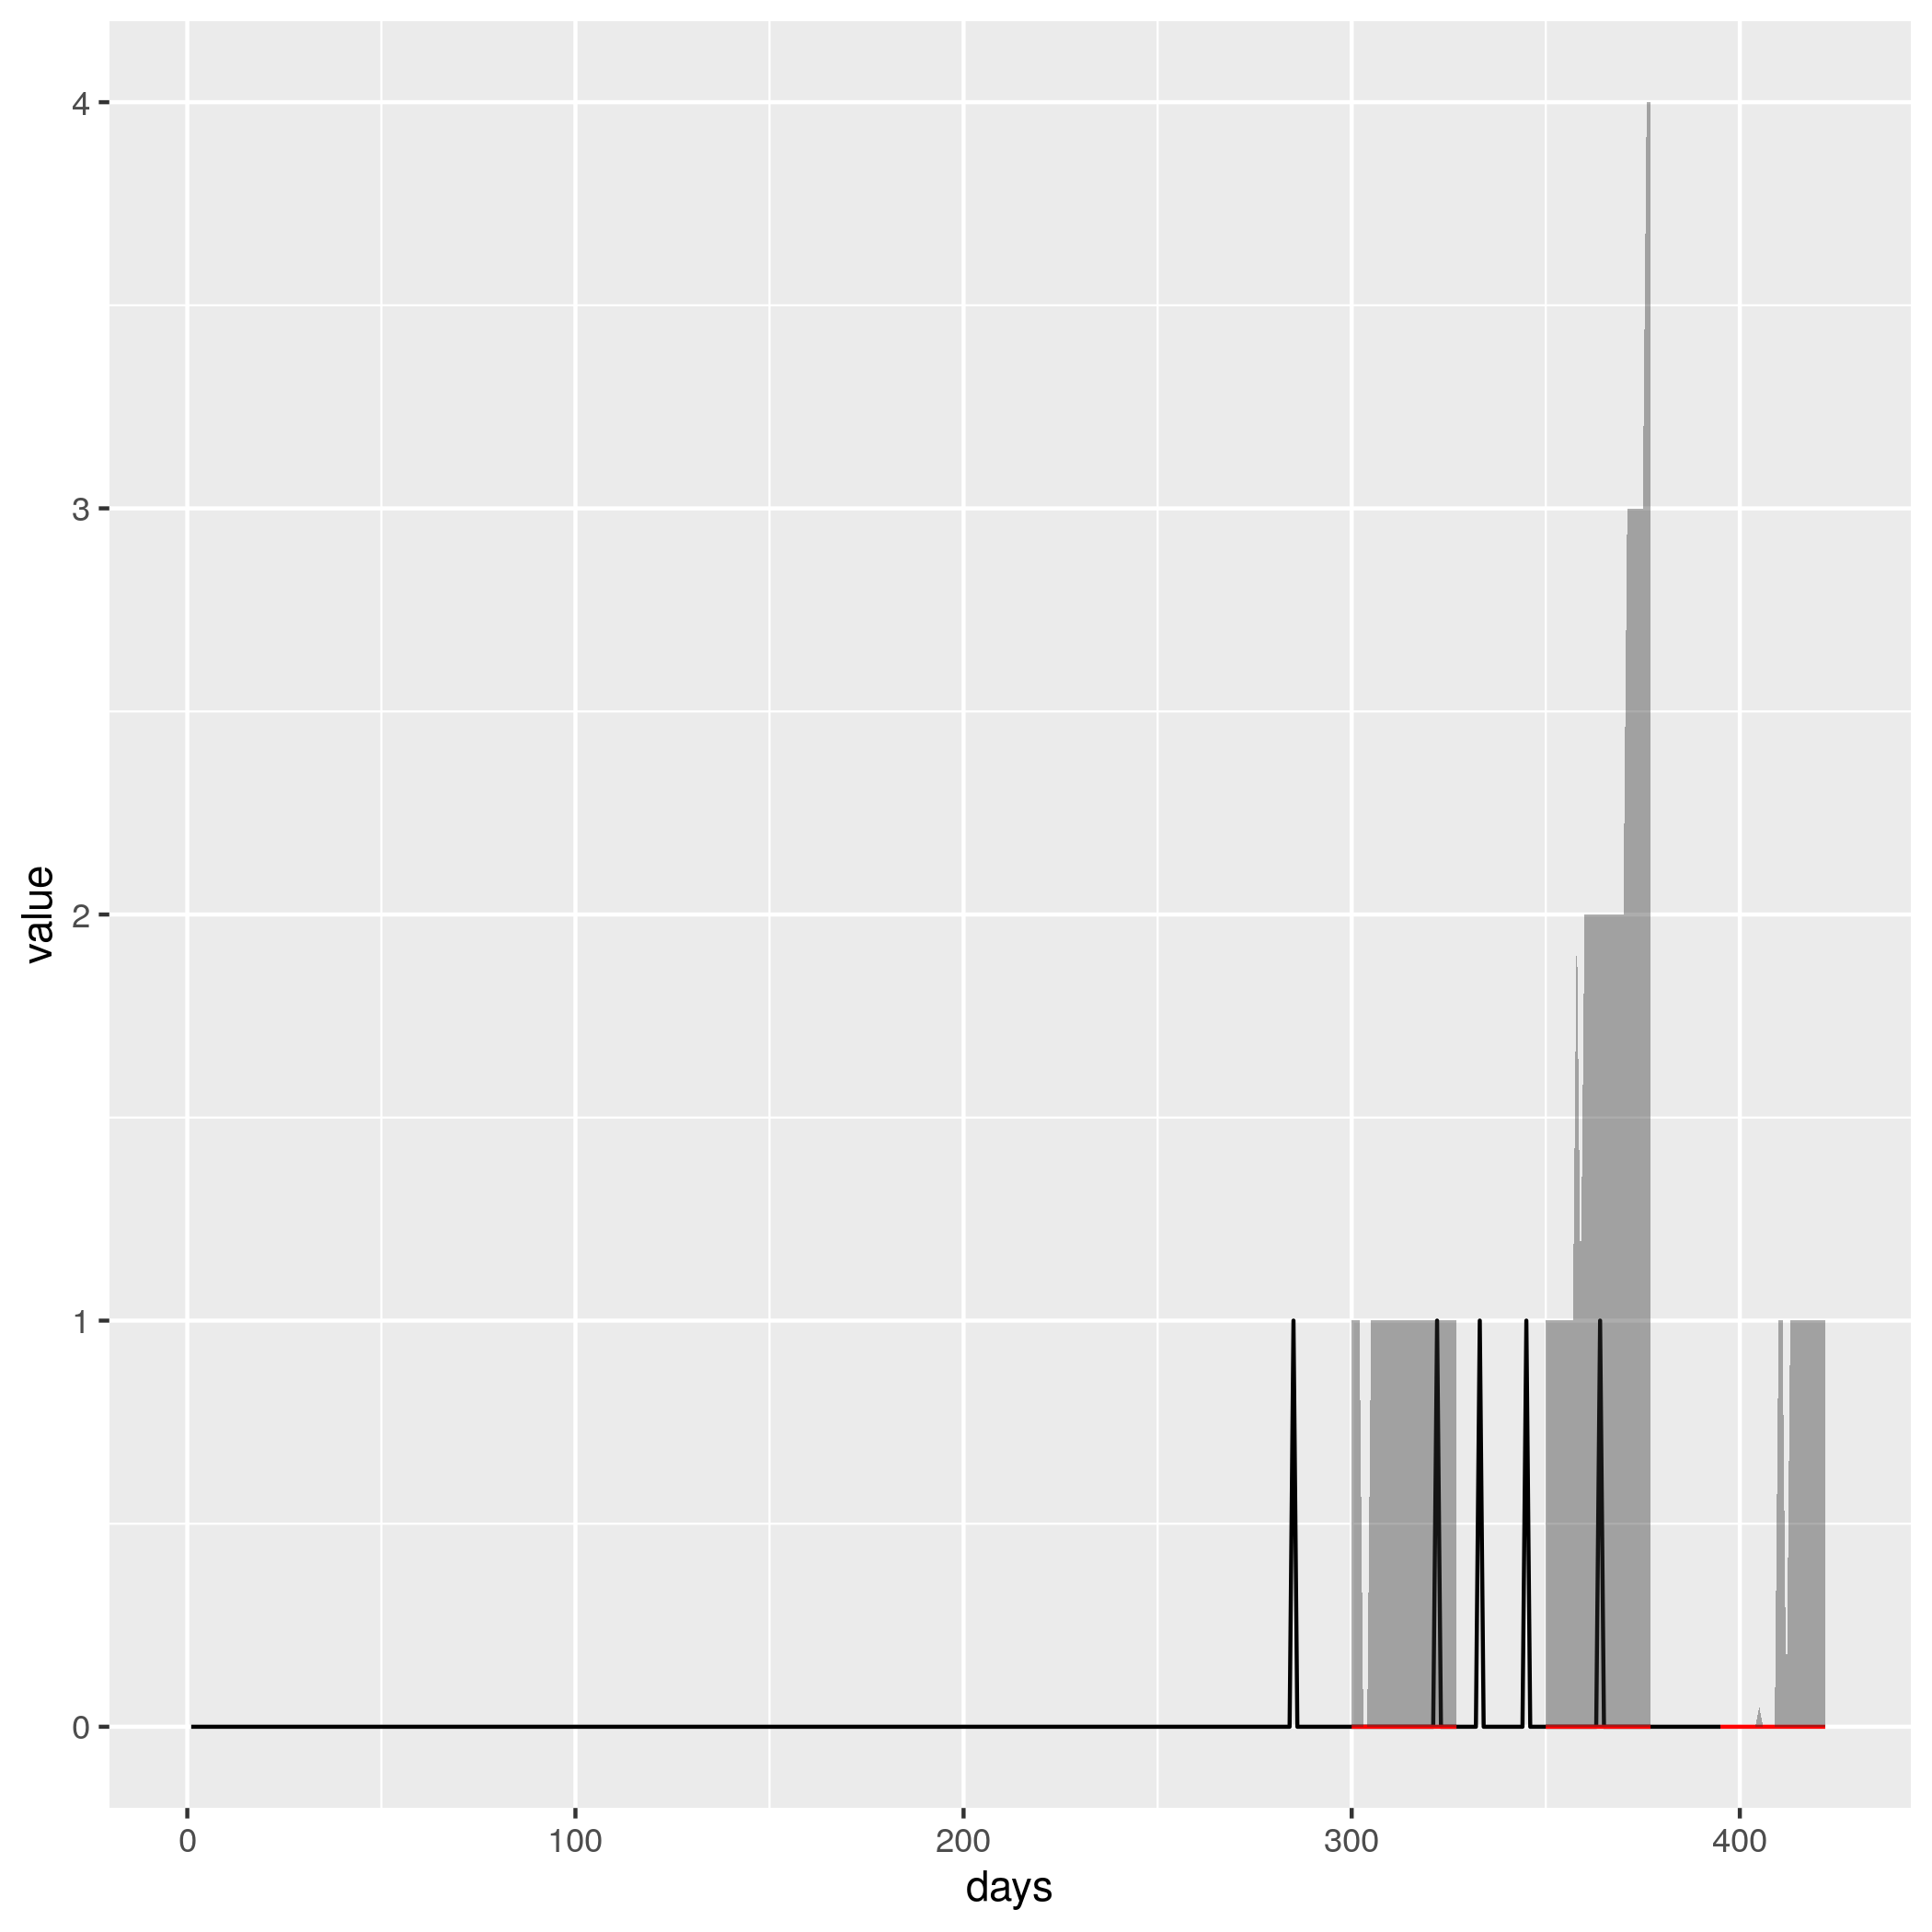
\includegraphics[width=0.9\linewidth, height=7cm]{../output/Alimbongo_predictions.png}  \caption{Forecasted and predicted incidence for the semilocal poisson model}\end{subfigure}

\begin{subfigure}{\textwidth}  \centering  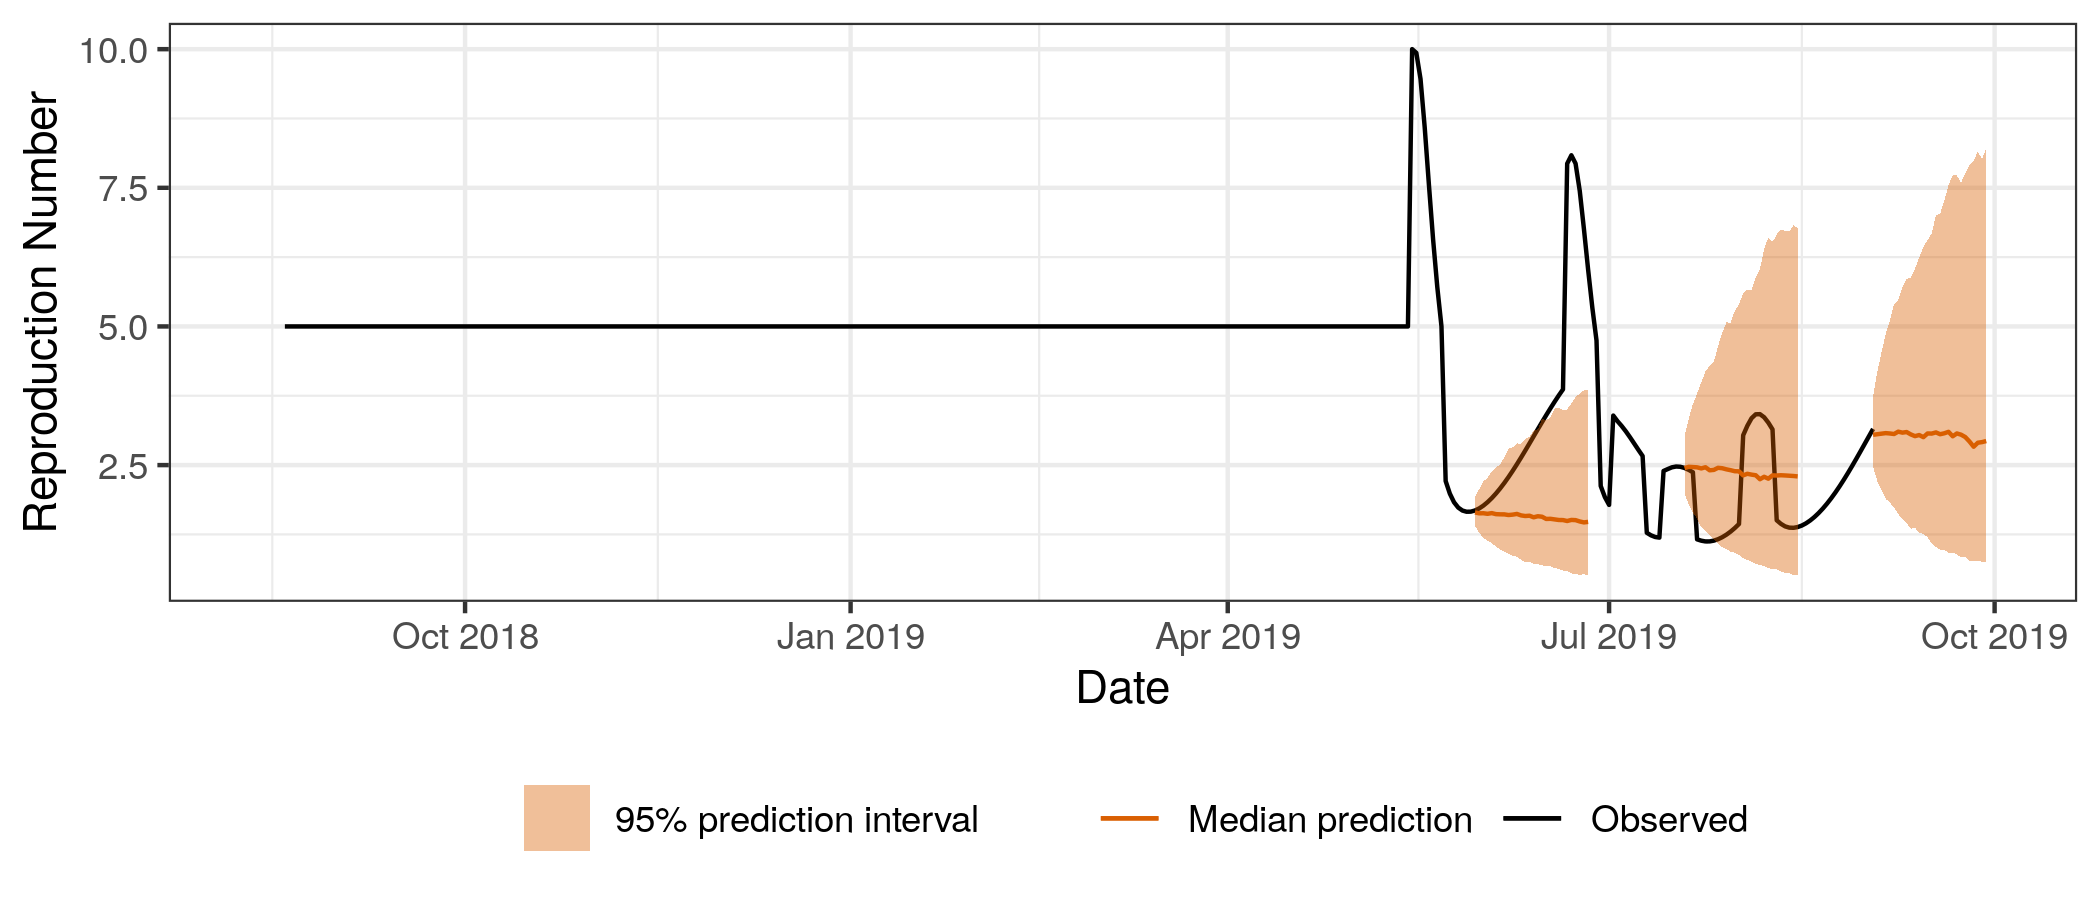
\includegraphics[width=0.9\linewidth, height=7cm]{../output/Alimbongo_Rs.png}  \caption{Forecasted and predicted repreoduction numbers for the semilocal poisson model}\end{subfigure}  \caption{Median forecast with 95 \% prediction intervals and observed values for incidence and reproduction number for the semilocal poisson model for Alimbongo.}\end{figure}

\begin{figure}[H]
\begin{subfigure}{0.5\textwidth}
  \centering
  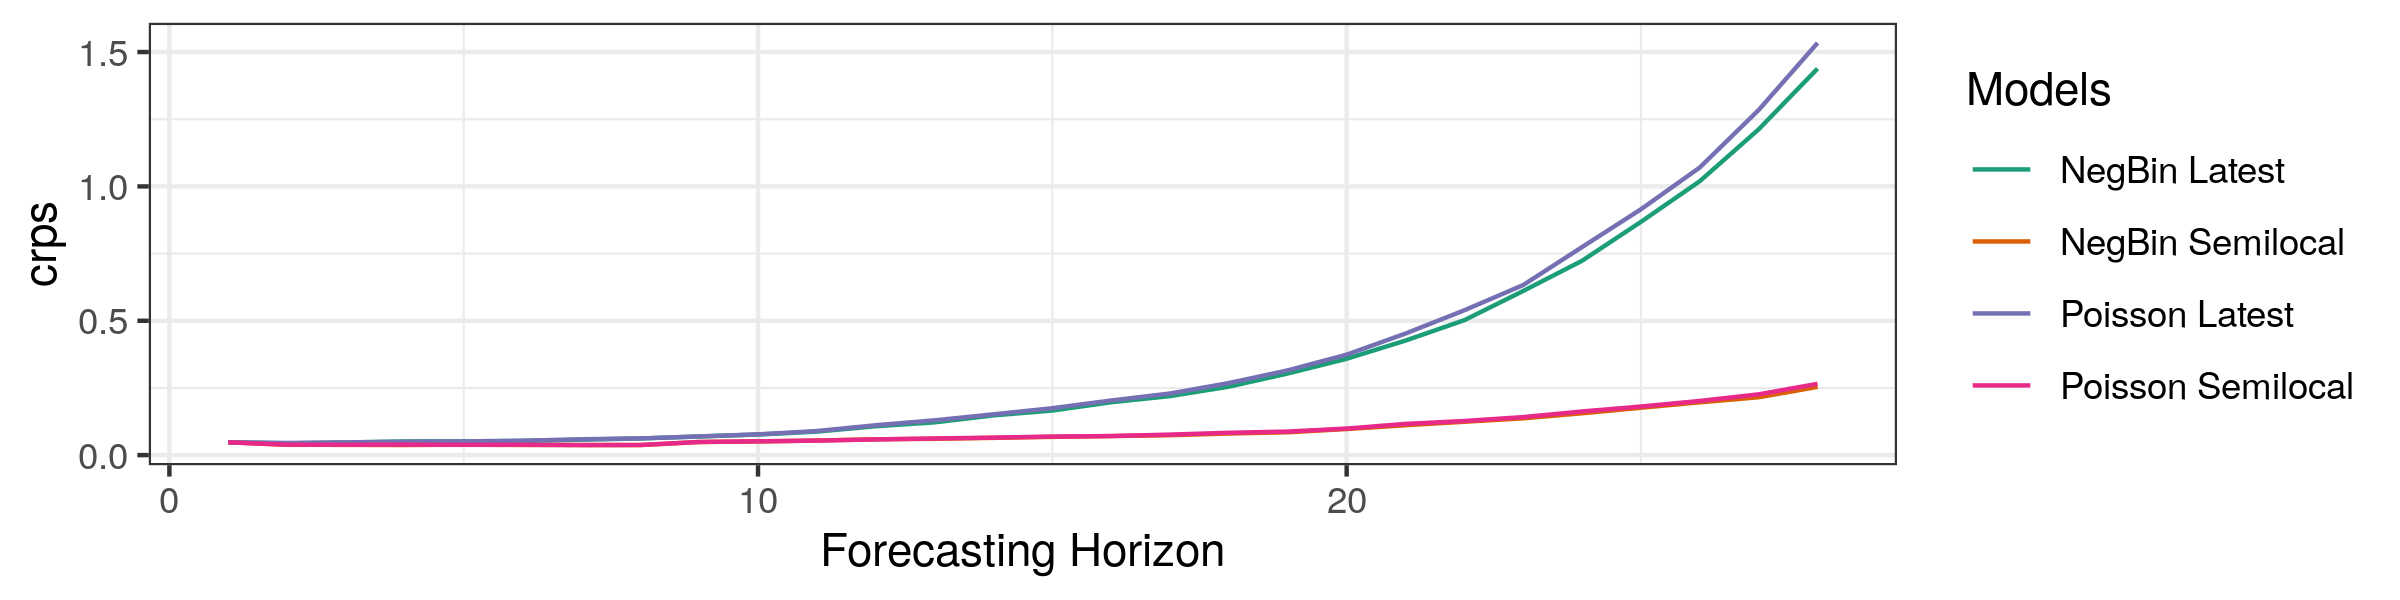
\includegraphics[width=\linewidth]{../output/Alimbongo_crps.png}  
  \caption{Contineously Ranked Probability Score}
  \label{fig:sub-first}
\end{subfigure}
\begin{subfigure}{0.5\textwidth}
  \centering
  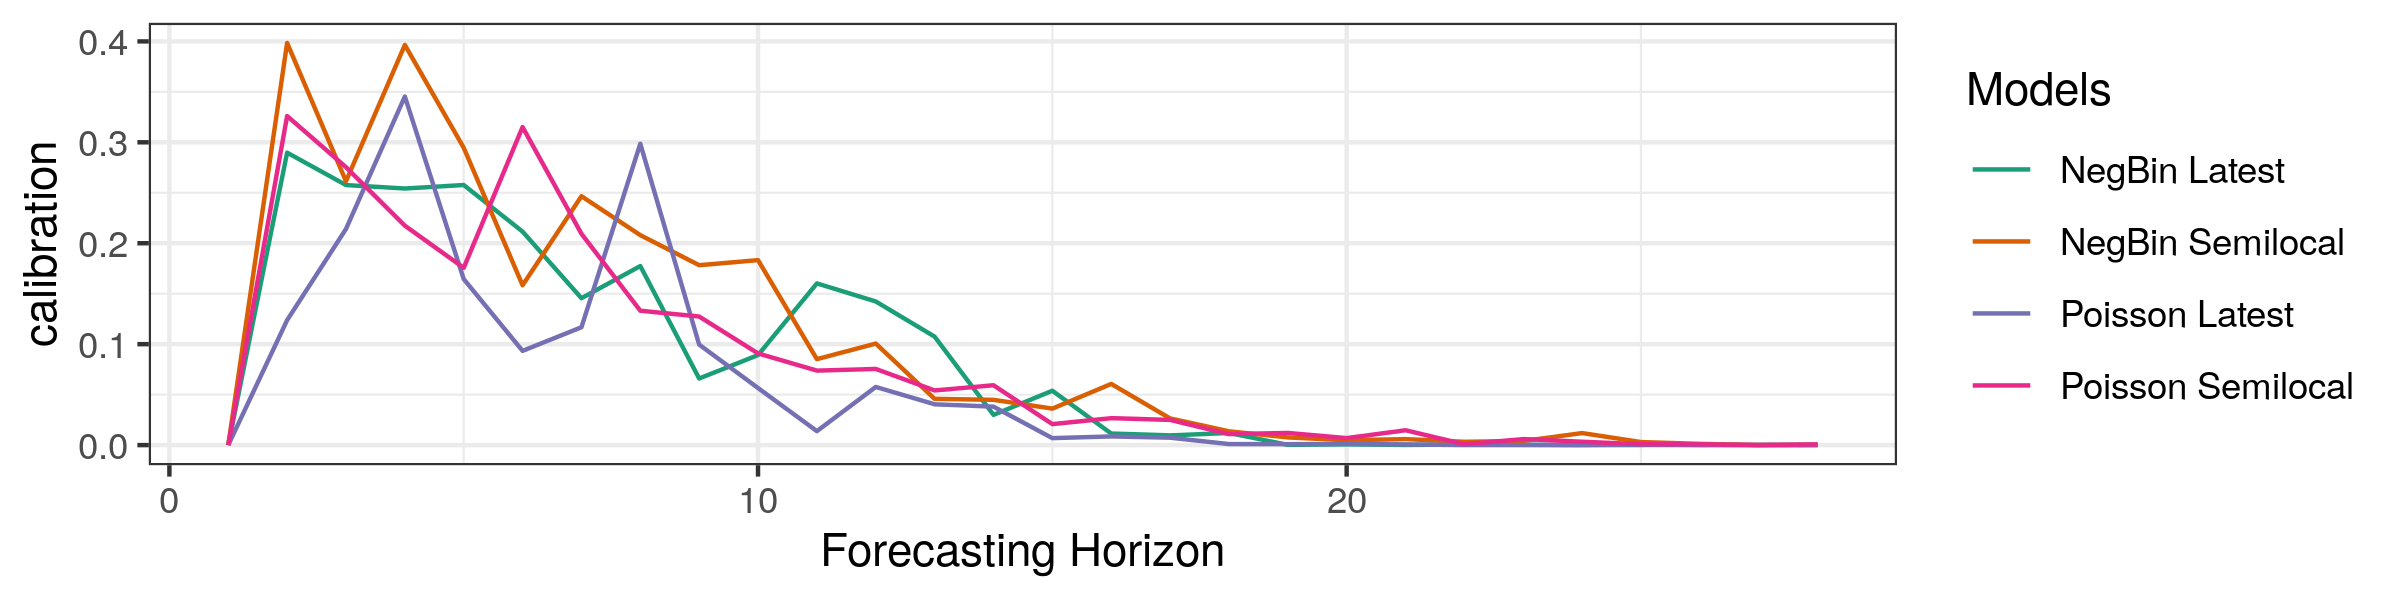
\includegraphics[width=\linewidth]{../output/Alimbongo_calibration.png}  
  \caption{Calibration p-value}
  \label{fig:sub-second}
\end{subfigure}

\begin{subfigure}{0.5\textwidth}
  \centering
  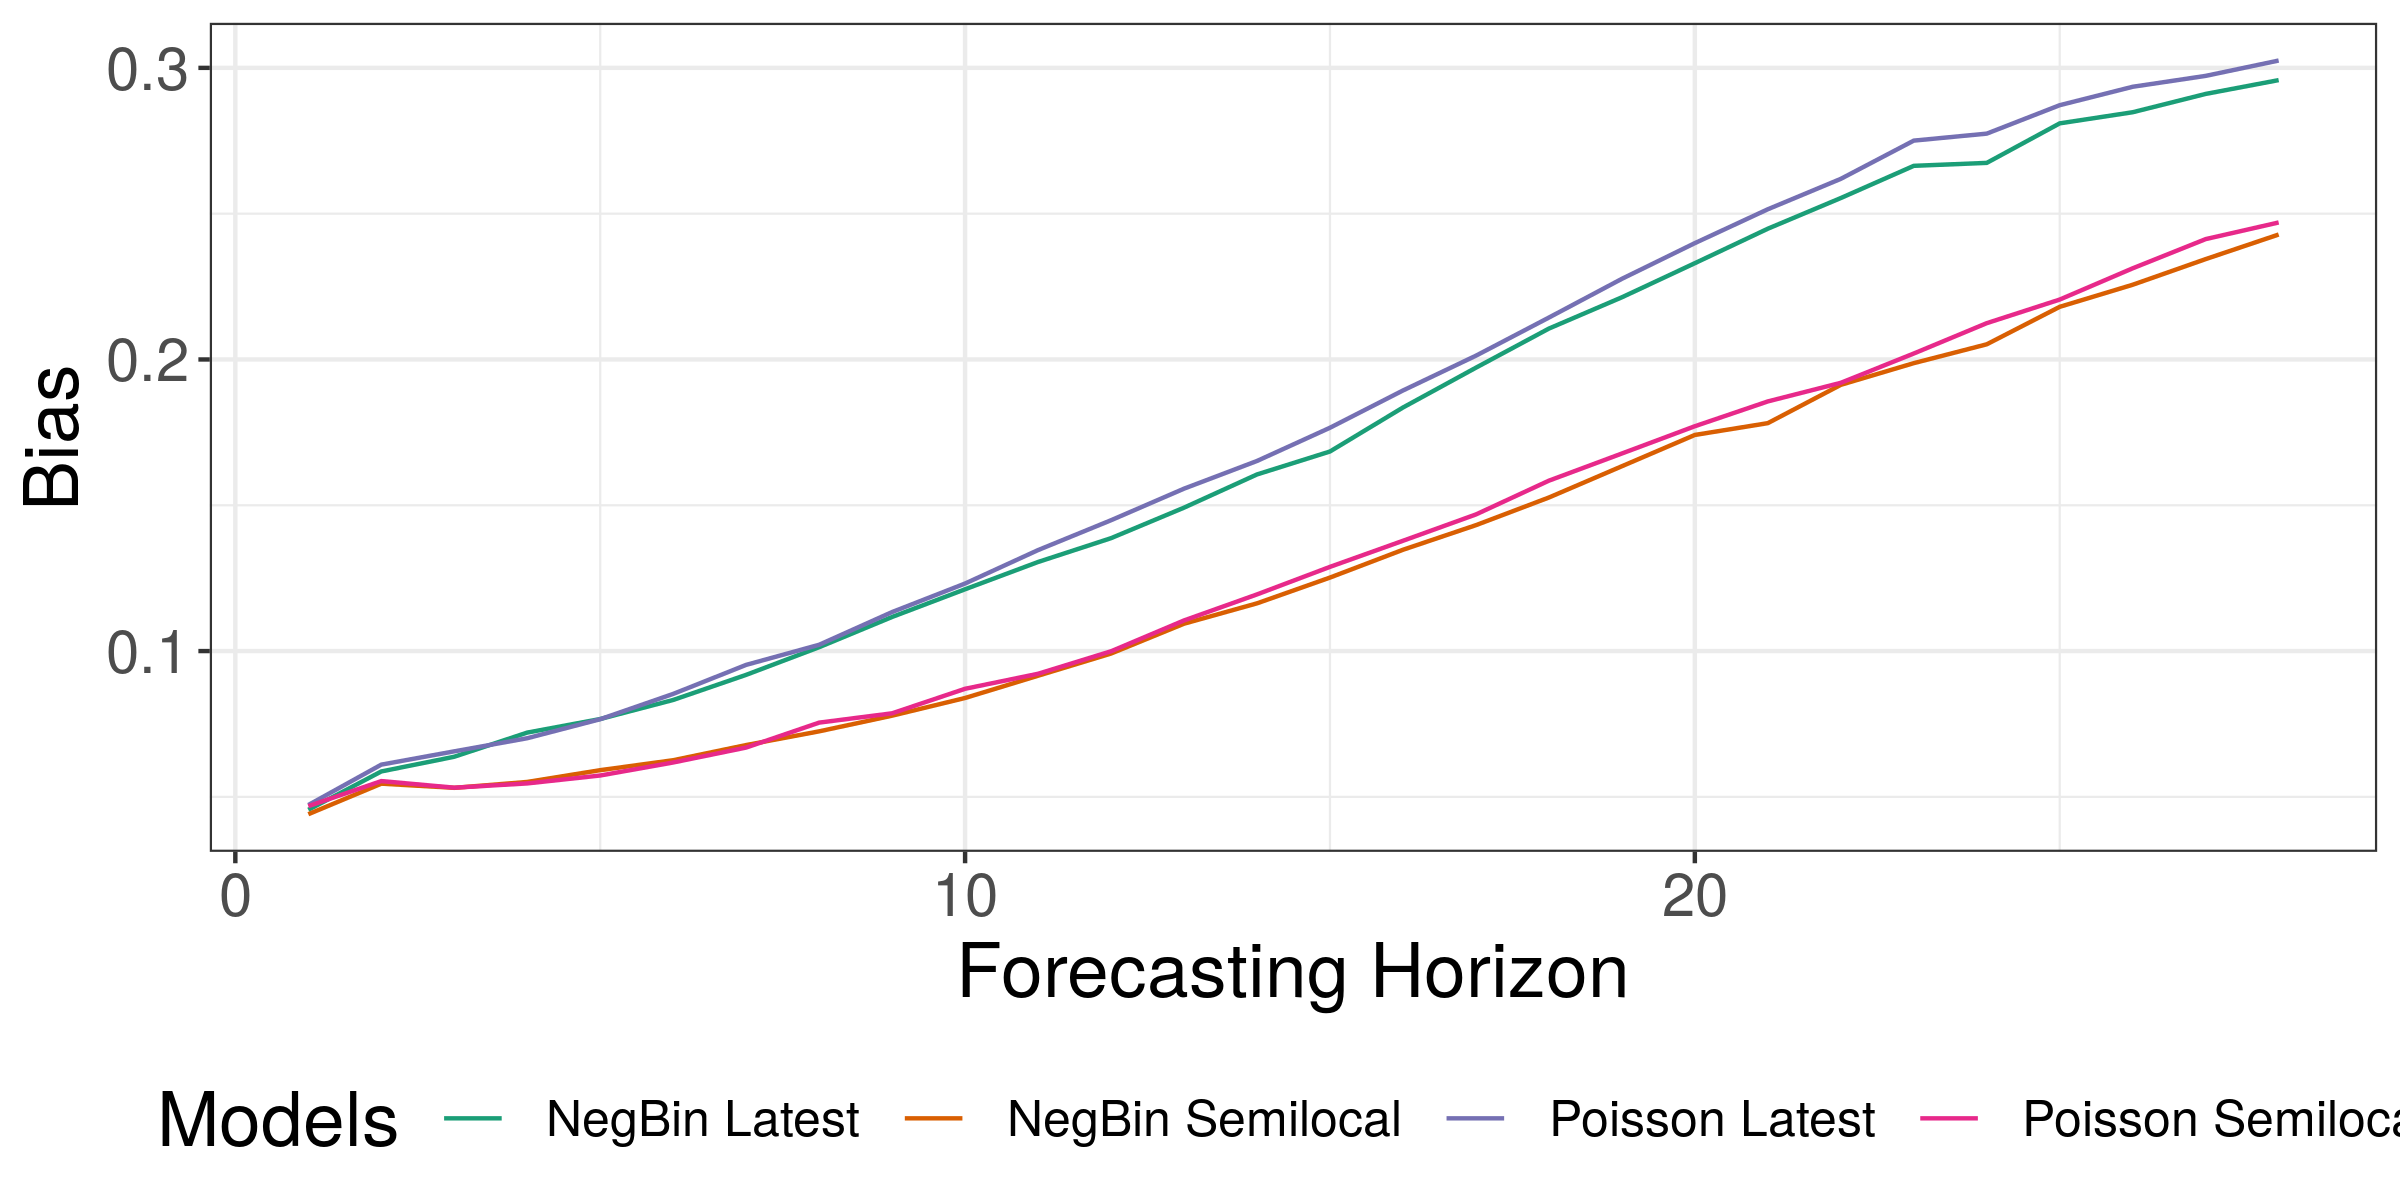
\includegraphics[width=\linewidth]{../output/Alimbongo_bias.png}  
  \caption{Bias}
  \label{fig:sub-third}
\end{subfigure}
\begin{subfigure}{0.5\textwidth}
  \centering
  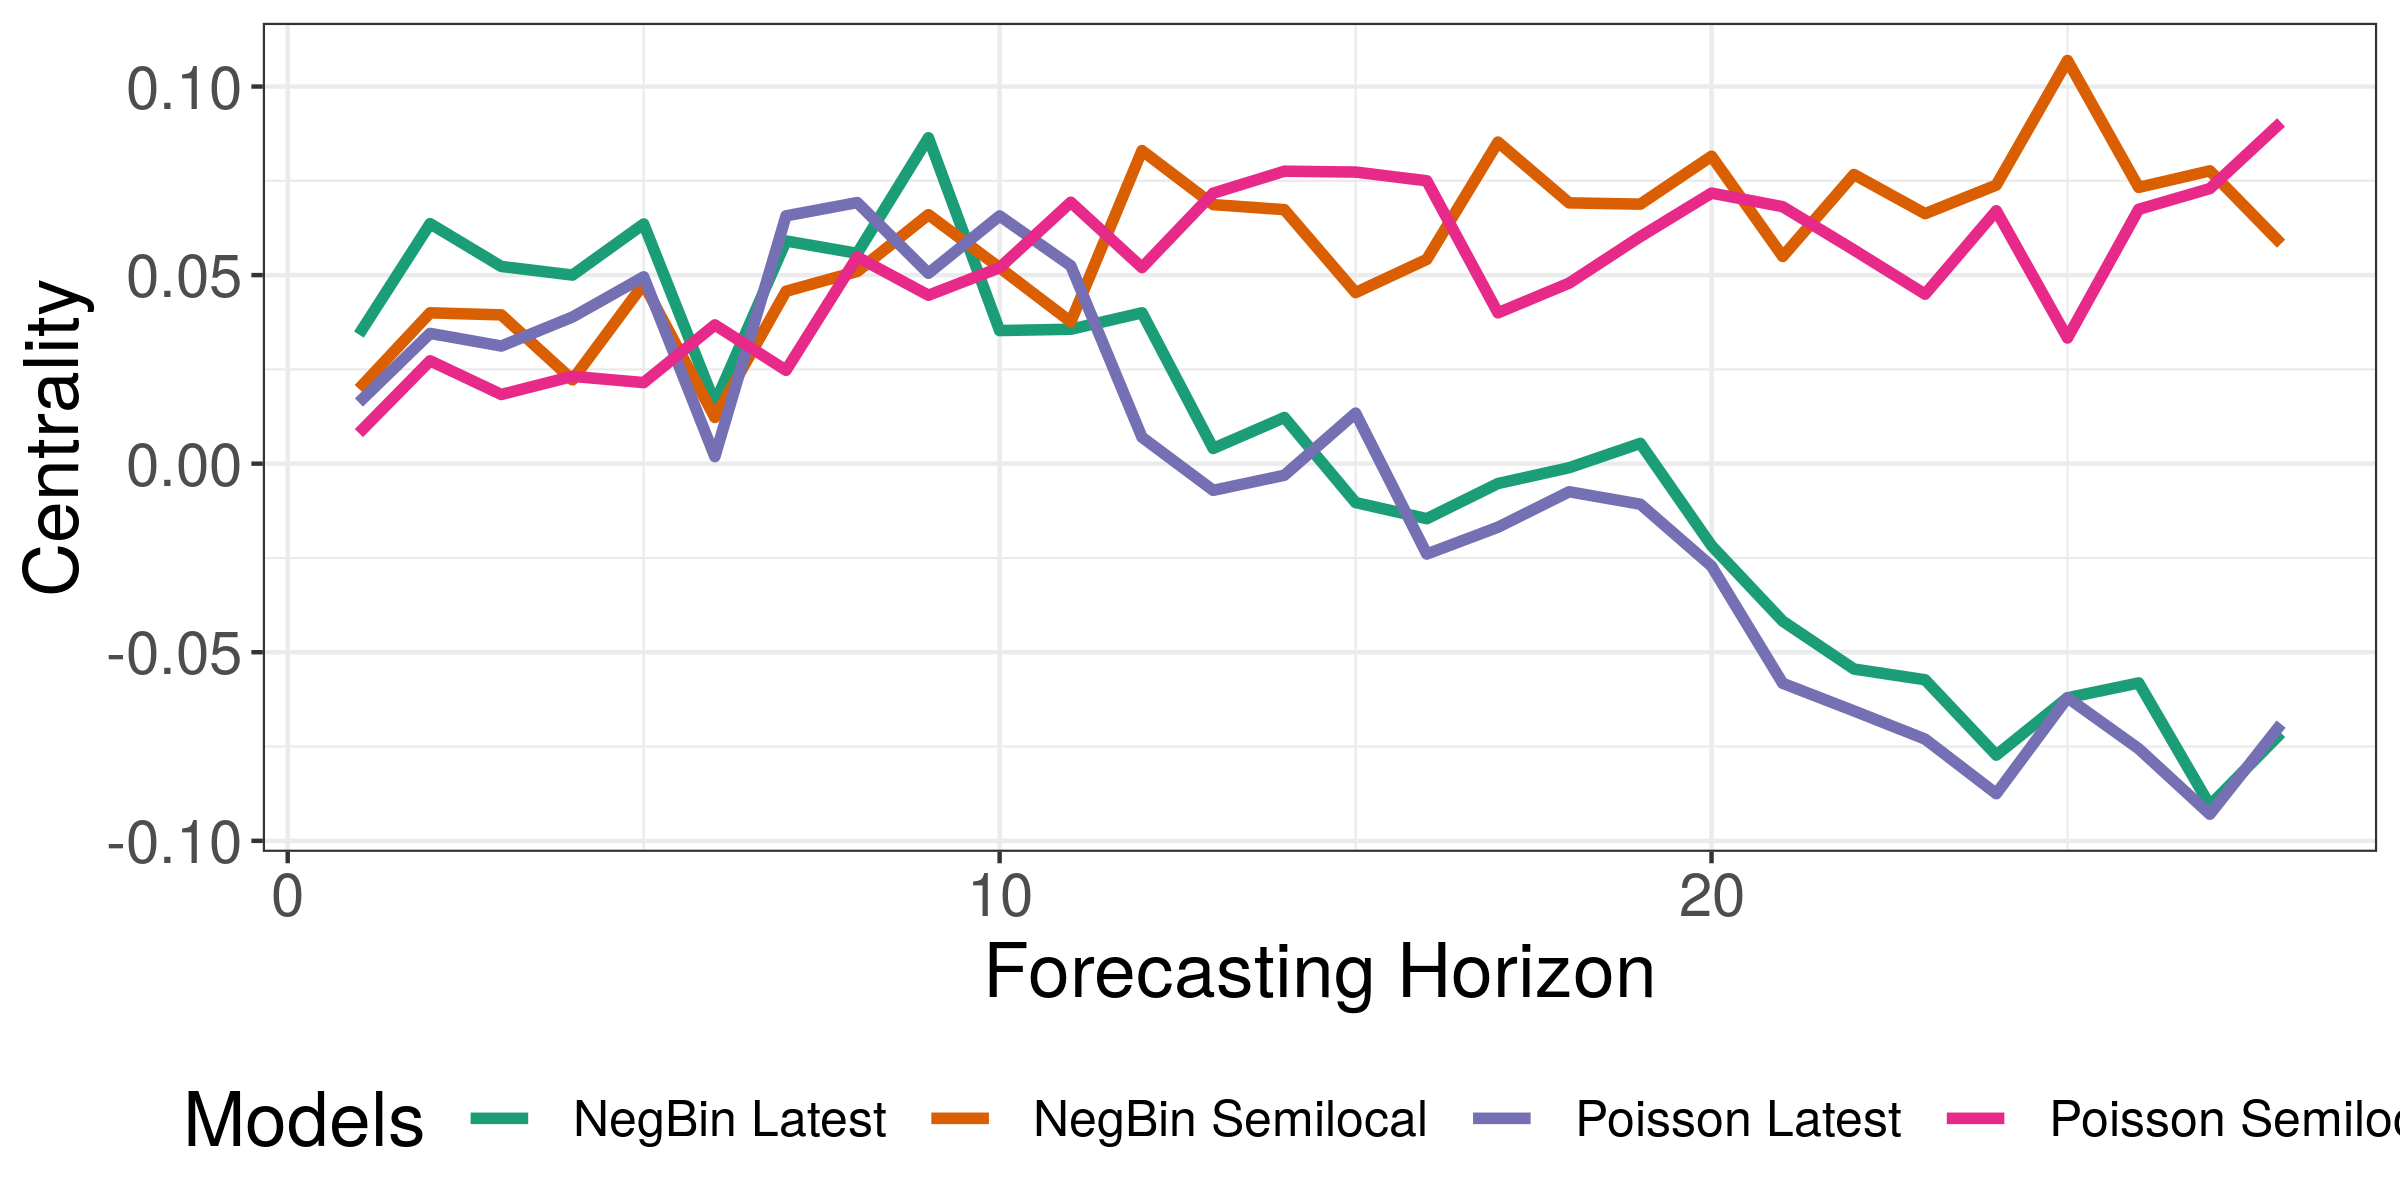
\includegraphics[width=\linewidth]{../output/Alimbongo_centrality.png}  
  \caption{Centrality of PIT values}
  \label{fig:nat_scores_4}
\end{subfigure}
  \caption{Scores for the entire outbreak as a function of the forecasting horizon.}

  \label{fig:nat_scores}
\end{figure}
 \section{ Beni }\begin{figure}[H]\begin{subfigure}{\textwidth}  \centering  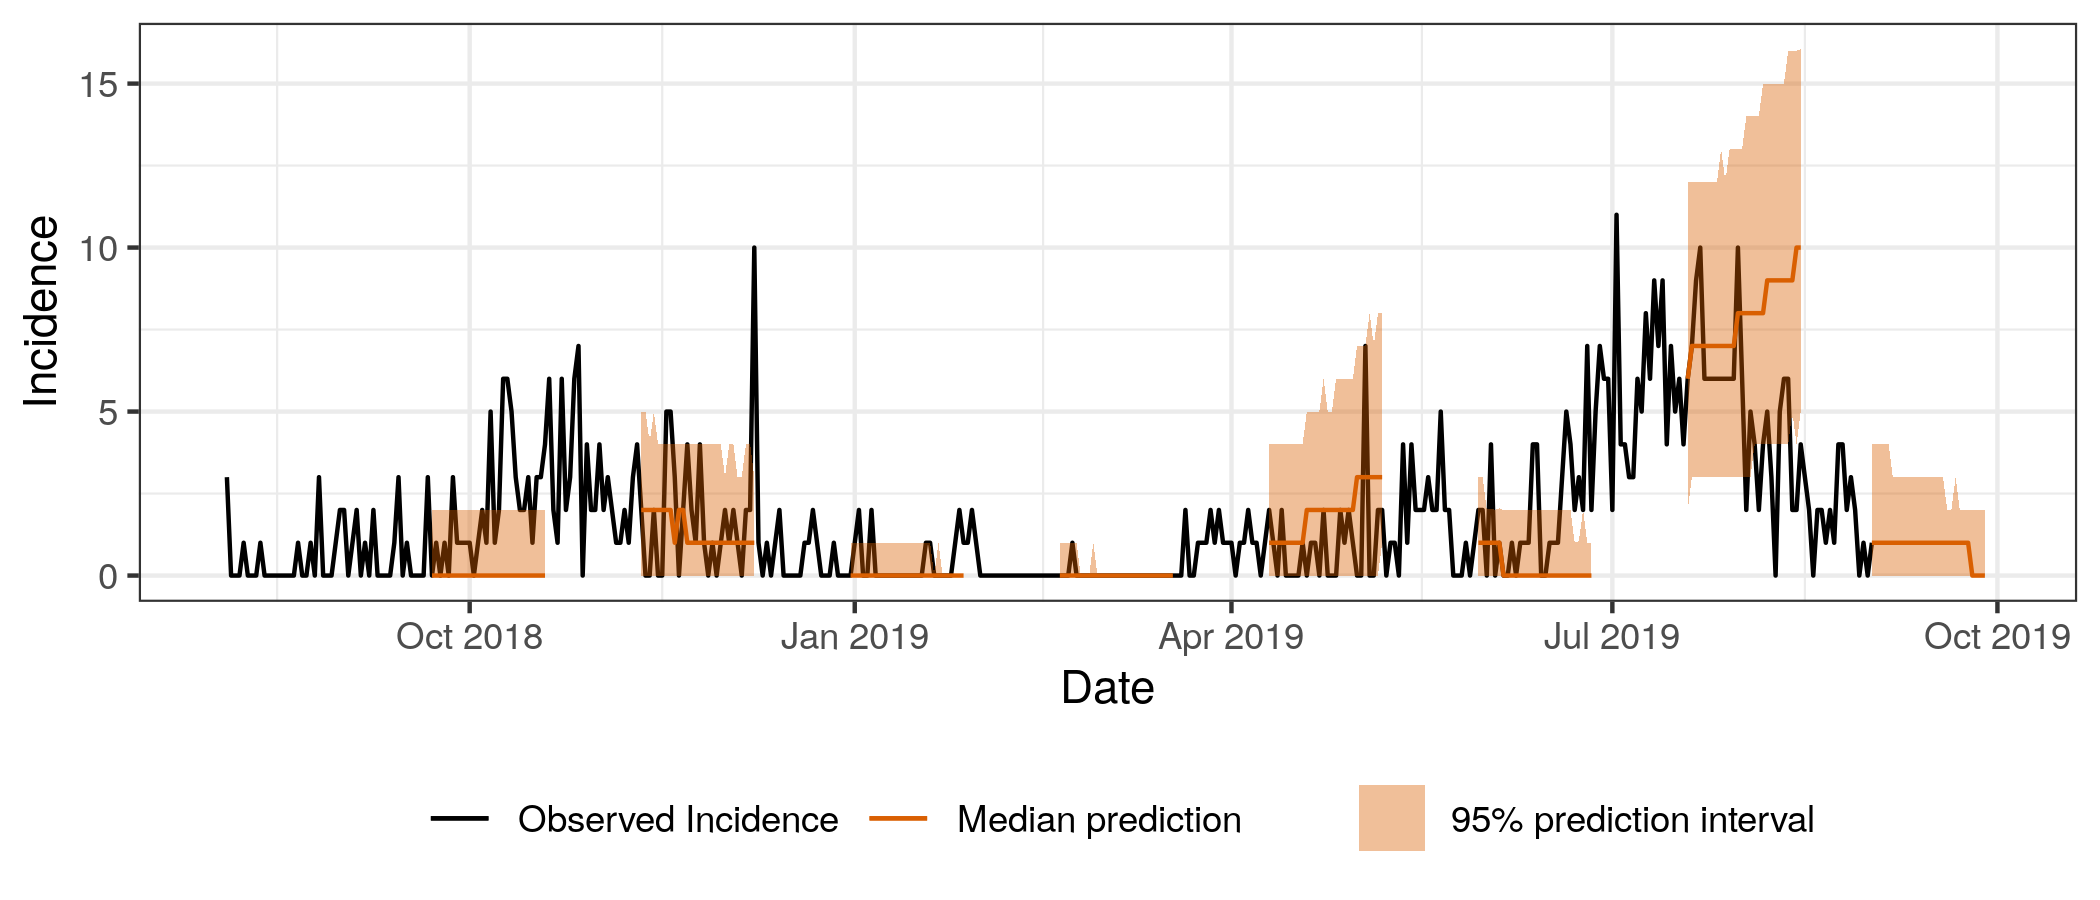
\includegraphics[width=0.9\linewidth, height=7cm]{../output/Beni_predictions.png}  \caption{Forecasted and predicted incidence for the semilocal poisson model}\end{subfigure}

\begin{subfigure}{\textwidth}  \centering  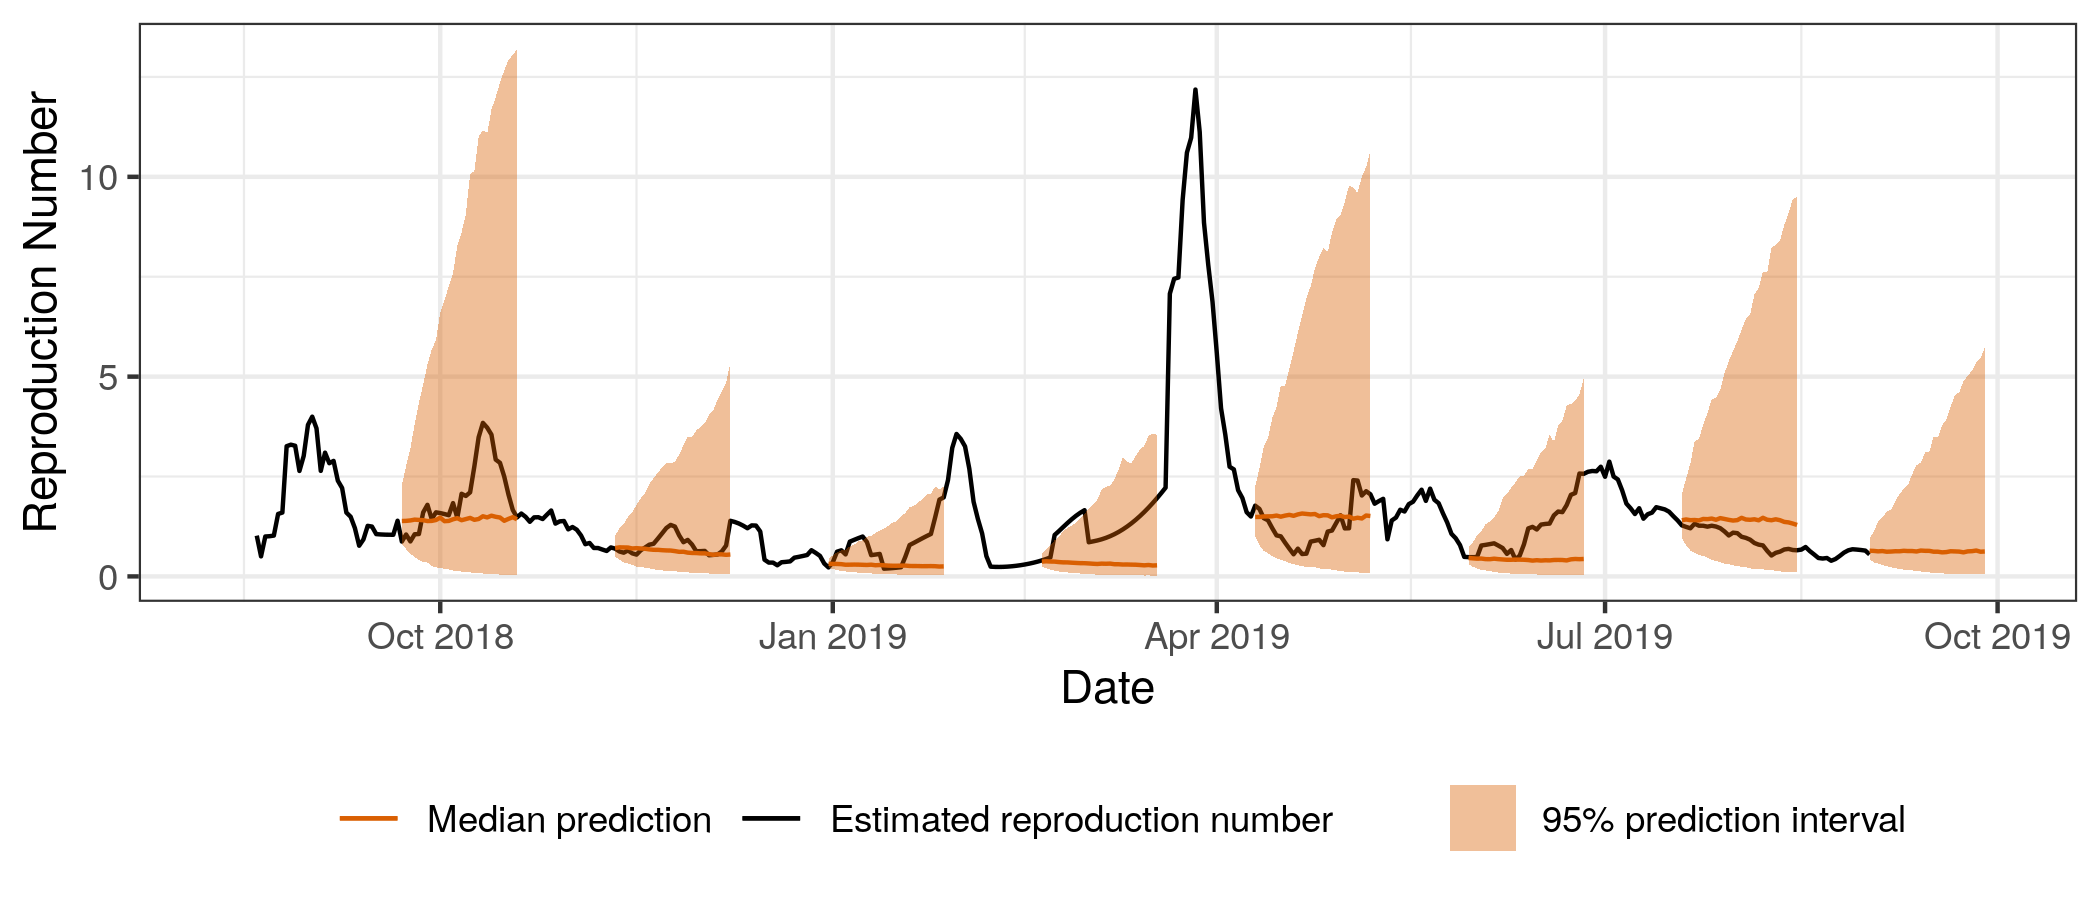
\includegraphics[width=0.9\linewidth, height=7cm]{../output/Beni_Rs.png}  \caption{Forecasted and predicted repreoduction numbers for the semilocal poisson model}\end{subfigure}  \caption{Median forecast with 95 \% prediction intervals and observed values for incidence and reproduction number for the semilocal poisson model for Beni.}\end{figure}

\begin{figure}[H]
\begin{subfigure}{0.5\textwidth}
  \centering
  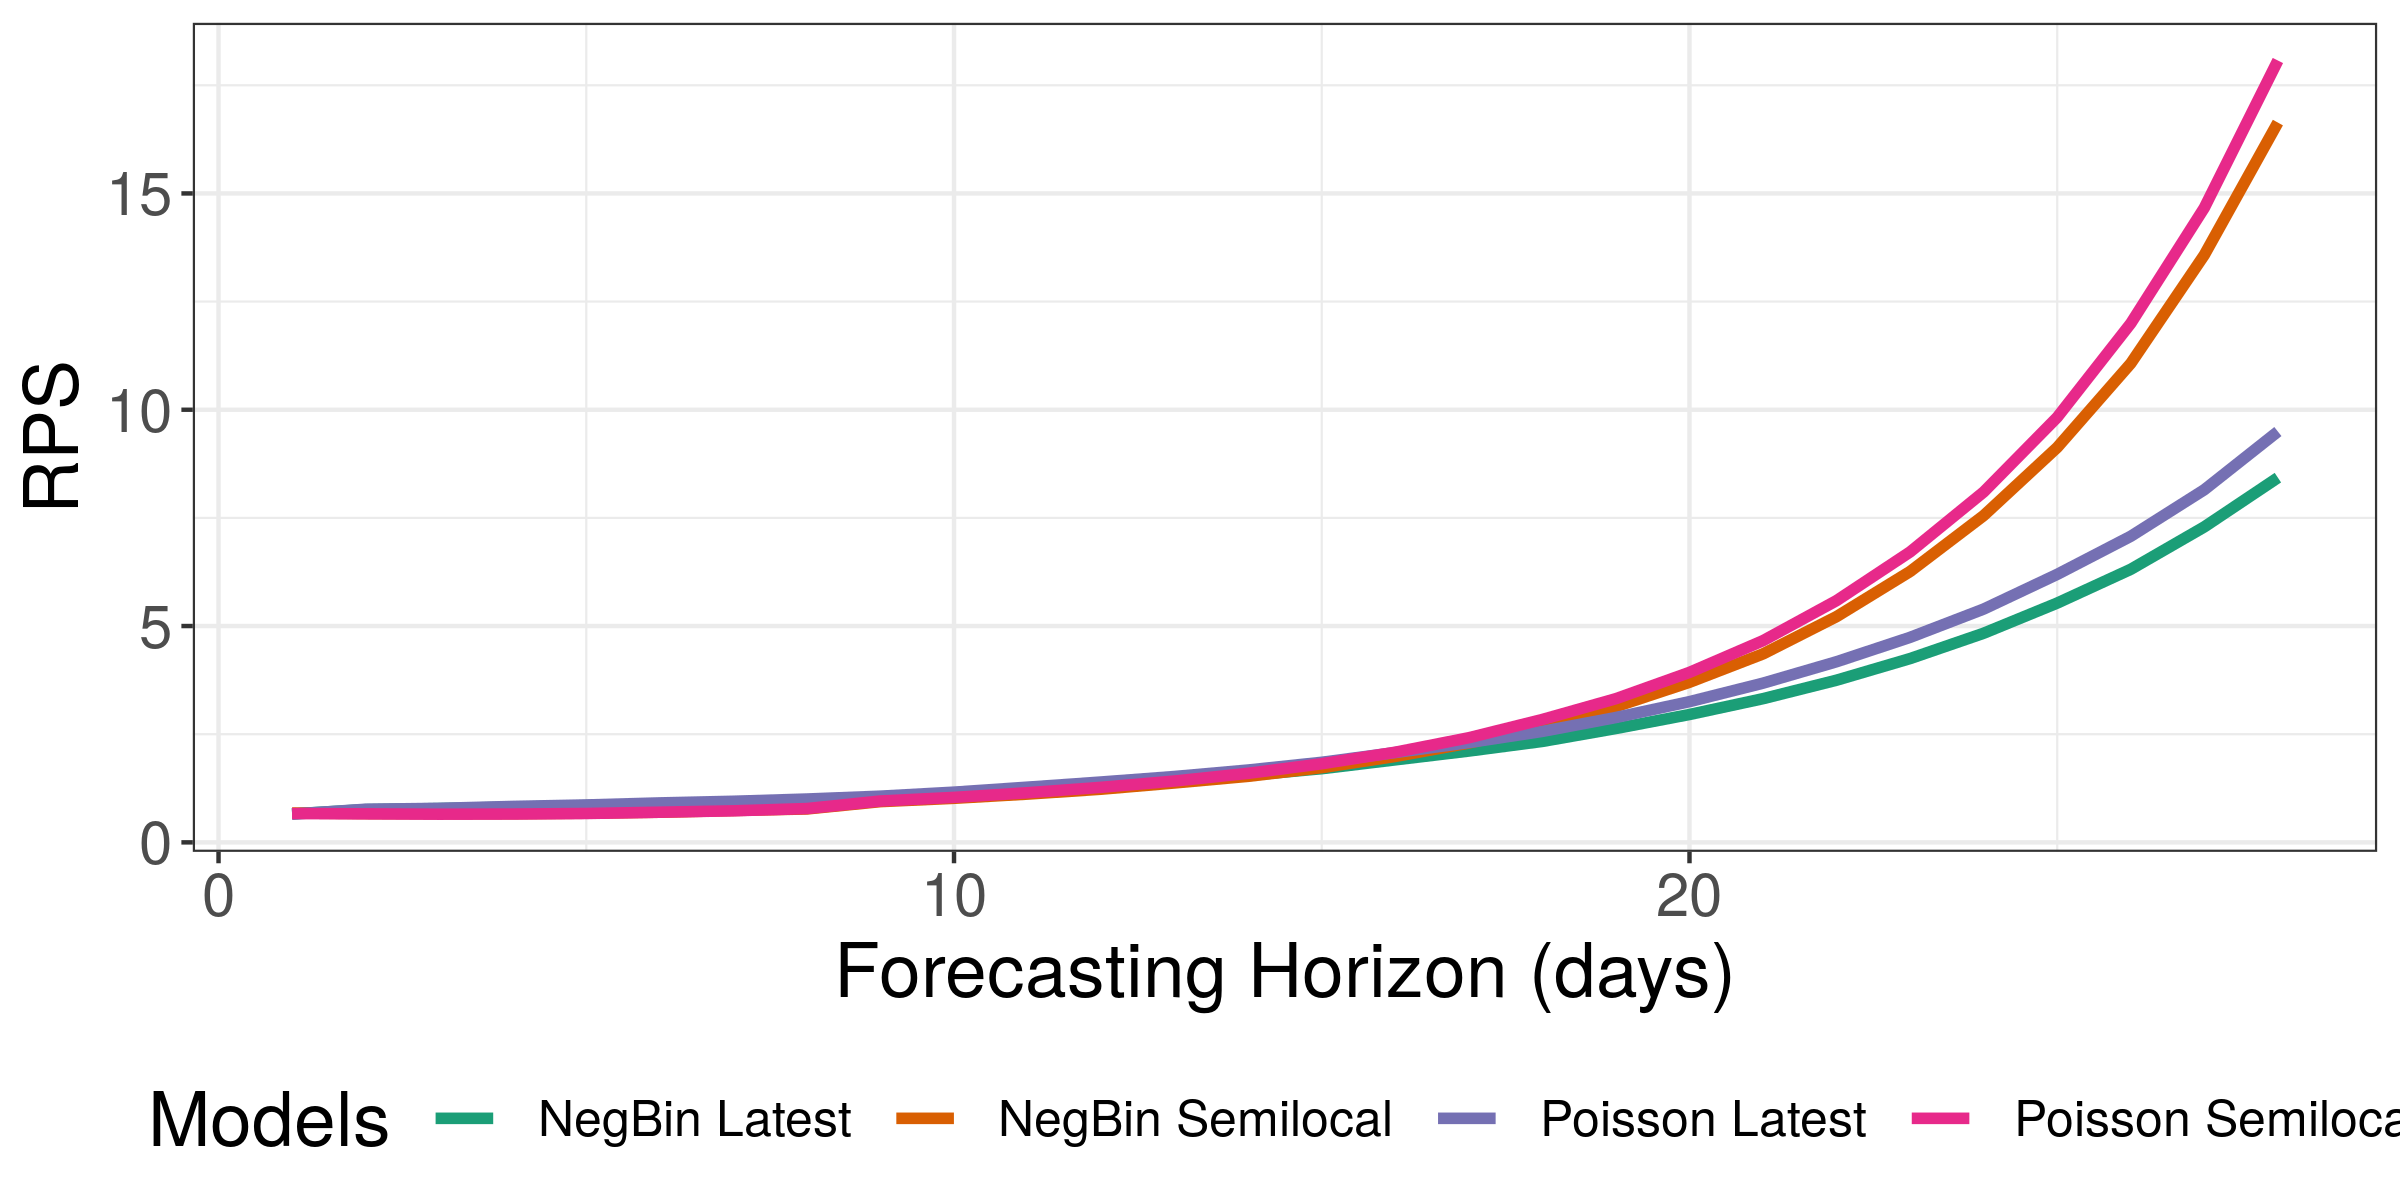
\includegraphics[width=\linewidth]{../output/Beni_crps.png}  
  \caption{Contineously Ranked Probability Score}
  \label{fig:sub-first}
\end{subfigure}
\begin{subfigure}{0.5\textwidth}
  \centering
  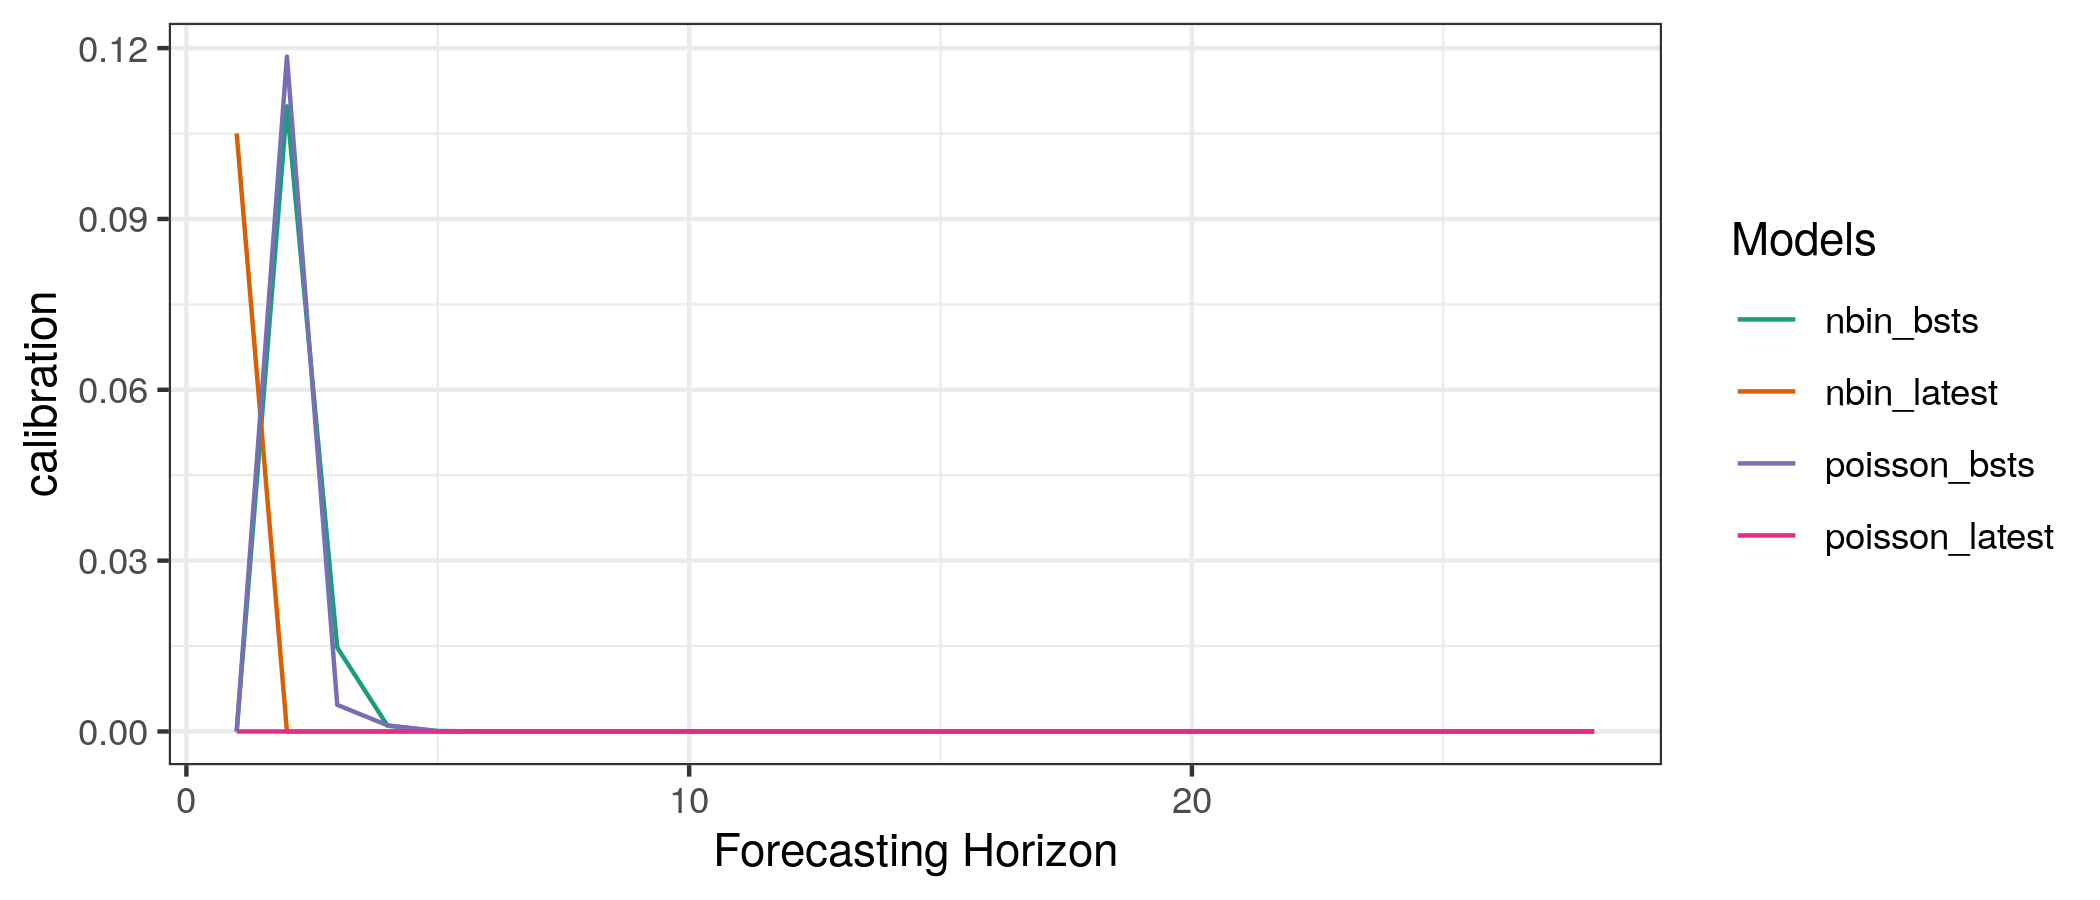
\includegraphics[width=\linewidth]{../output/Beni_calibration.png}  
  \caption{Calibration p-value}
  \label{fig:sub-second}
\end{subfigure}

\begin{subfigure}{0.5\textwidth}
  \centering
  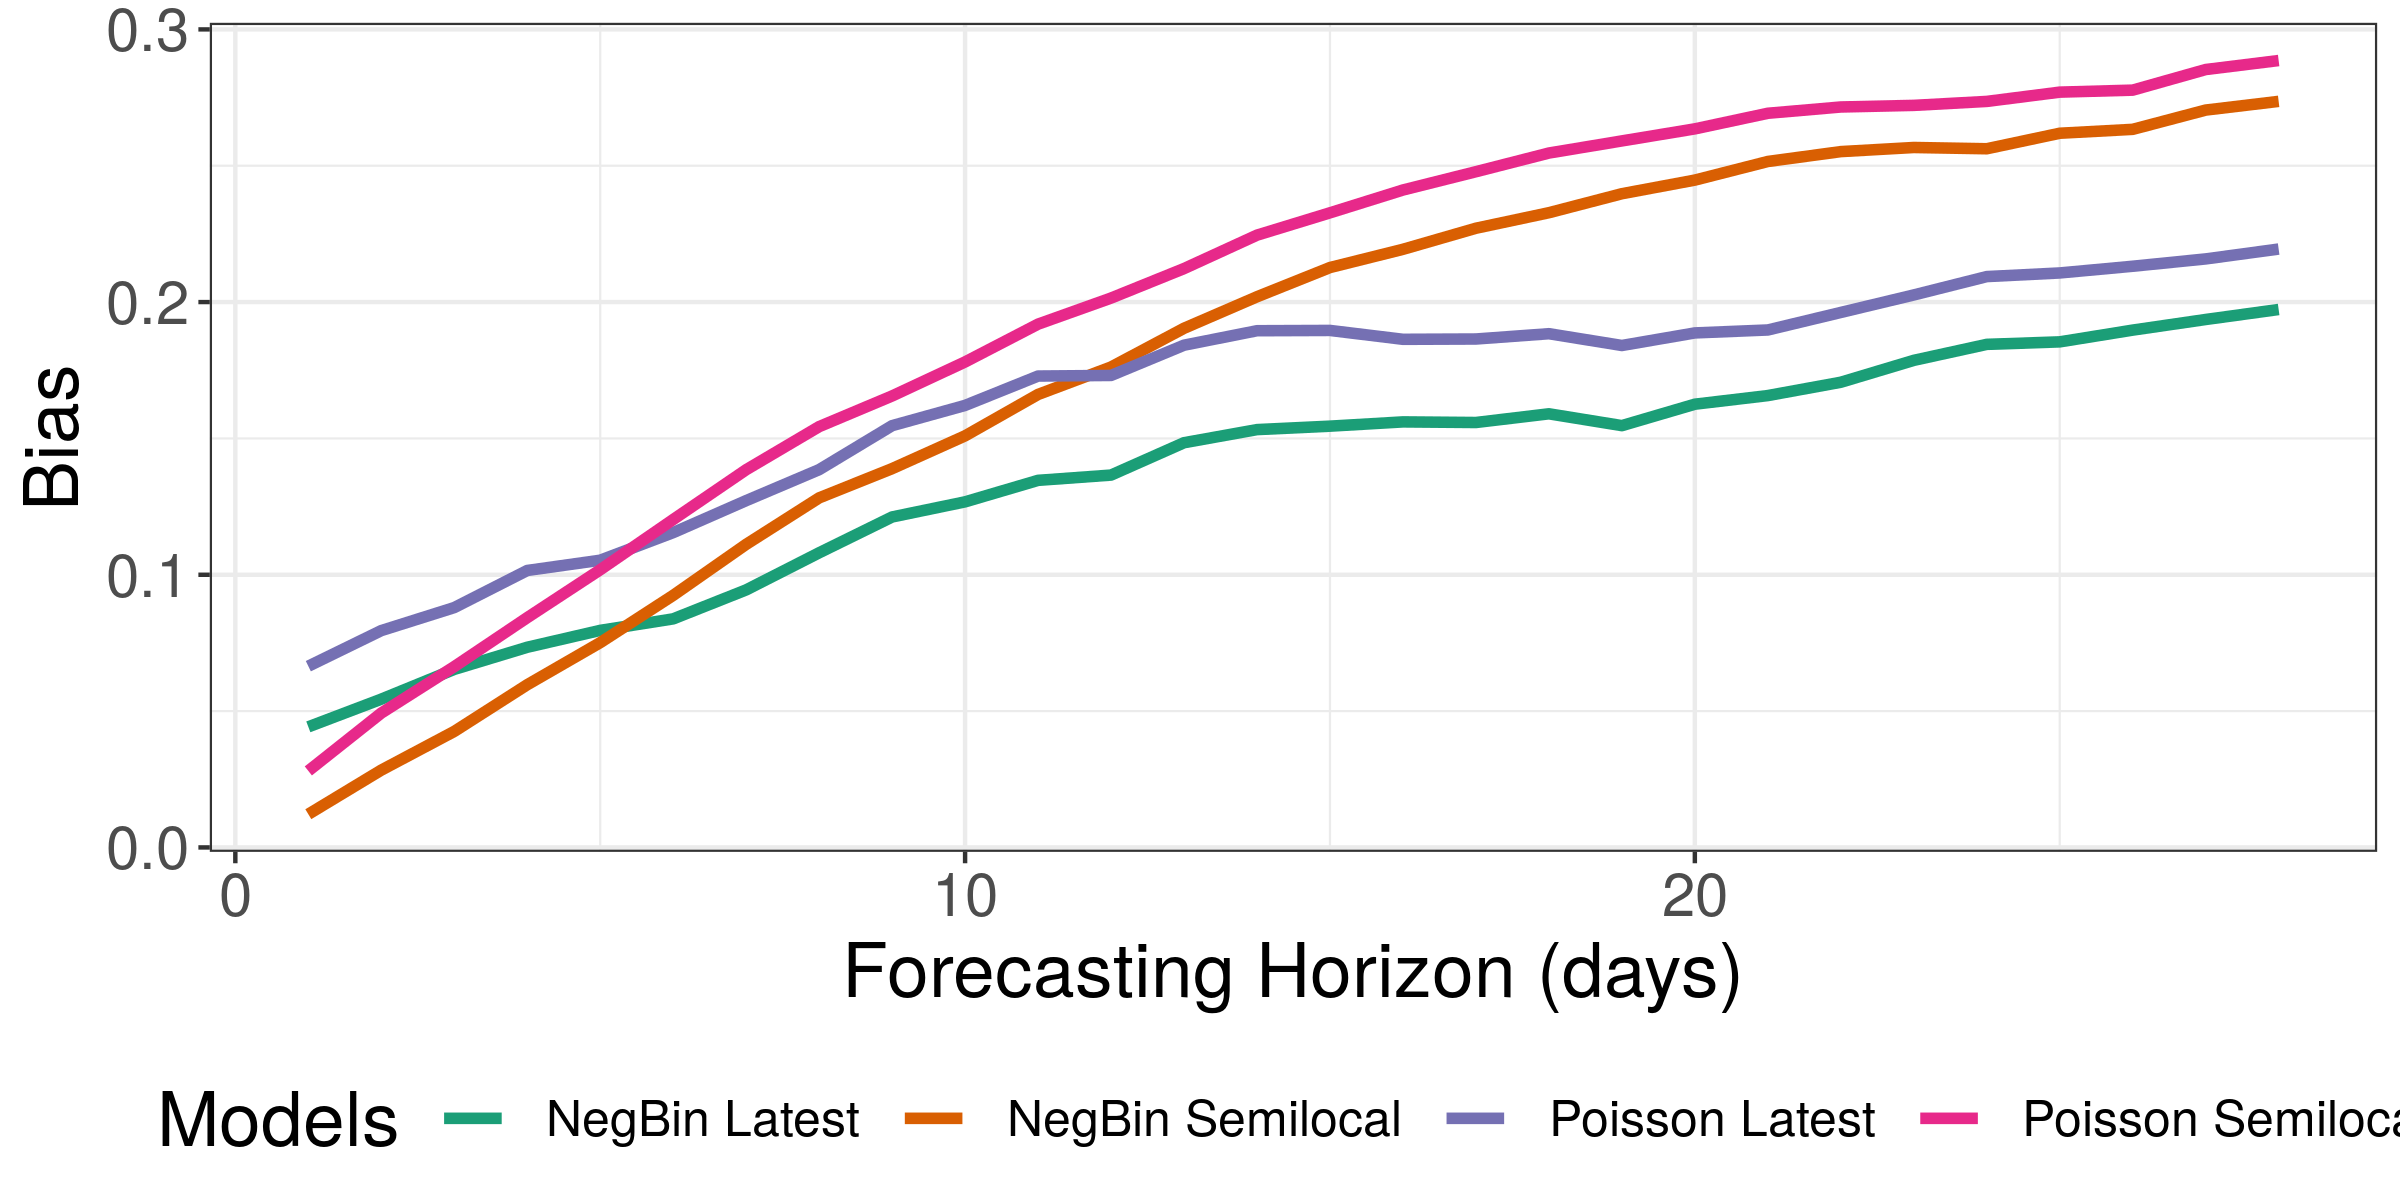
\includegraphics[width=\linewidth]{../output/Beni_bias.png}  
  \caption{Bias}
  \label{fig:sub-third}
\end{subfigure}
\begin{subfigure}{0.5\textwidth}
  \centering
  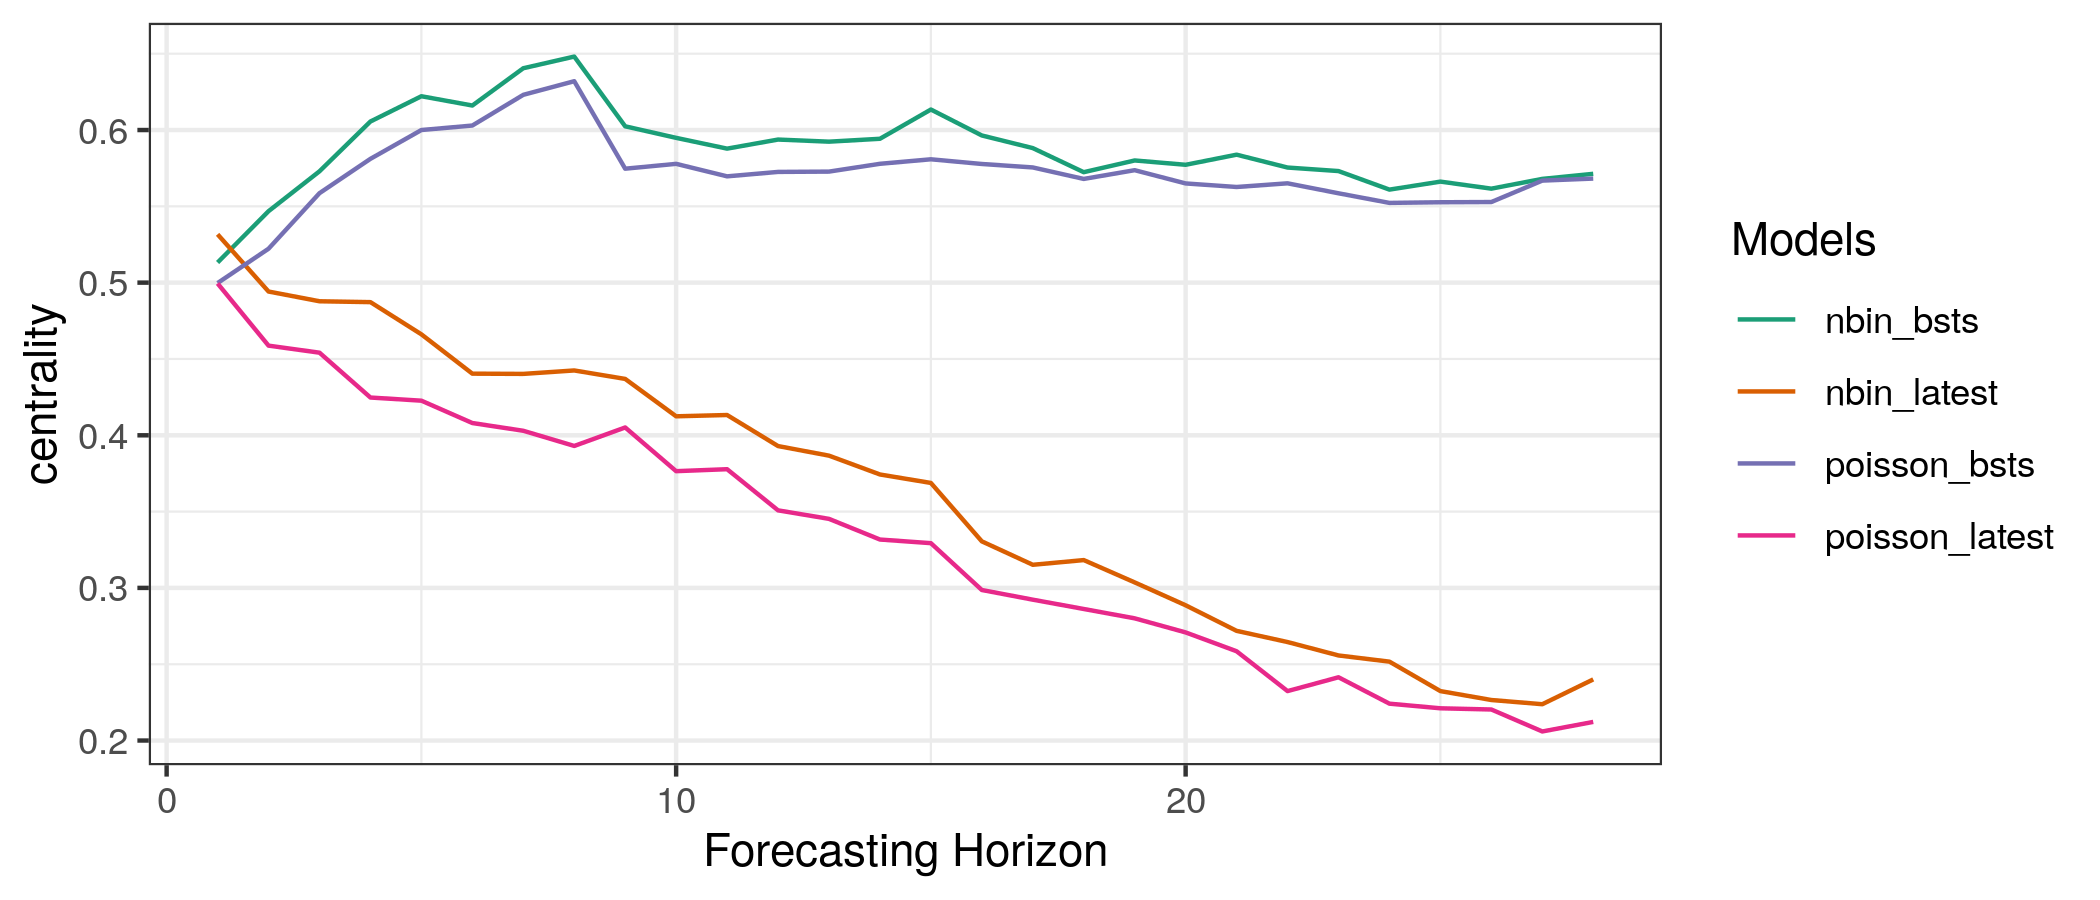
\includegraphics[width=\linewidth]{../output/Beni_centrality.png}  
  \caption{Centrality of PIT values}
  \label{fig:nat_scores_4}
\end{subfigure}
  \caption{Scores for the entire outbreak as a function of the forecasting horizon.}

  \label{fig:nat_scores}
\end{figure}
 \section{ Biena }\begin{figure}[H]\begin{subfigure}{\textwidth}  \centering  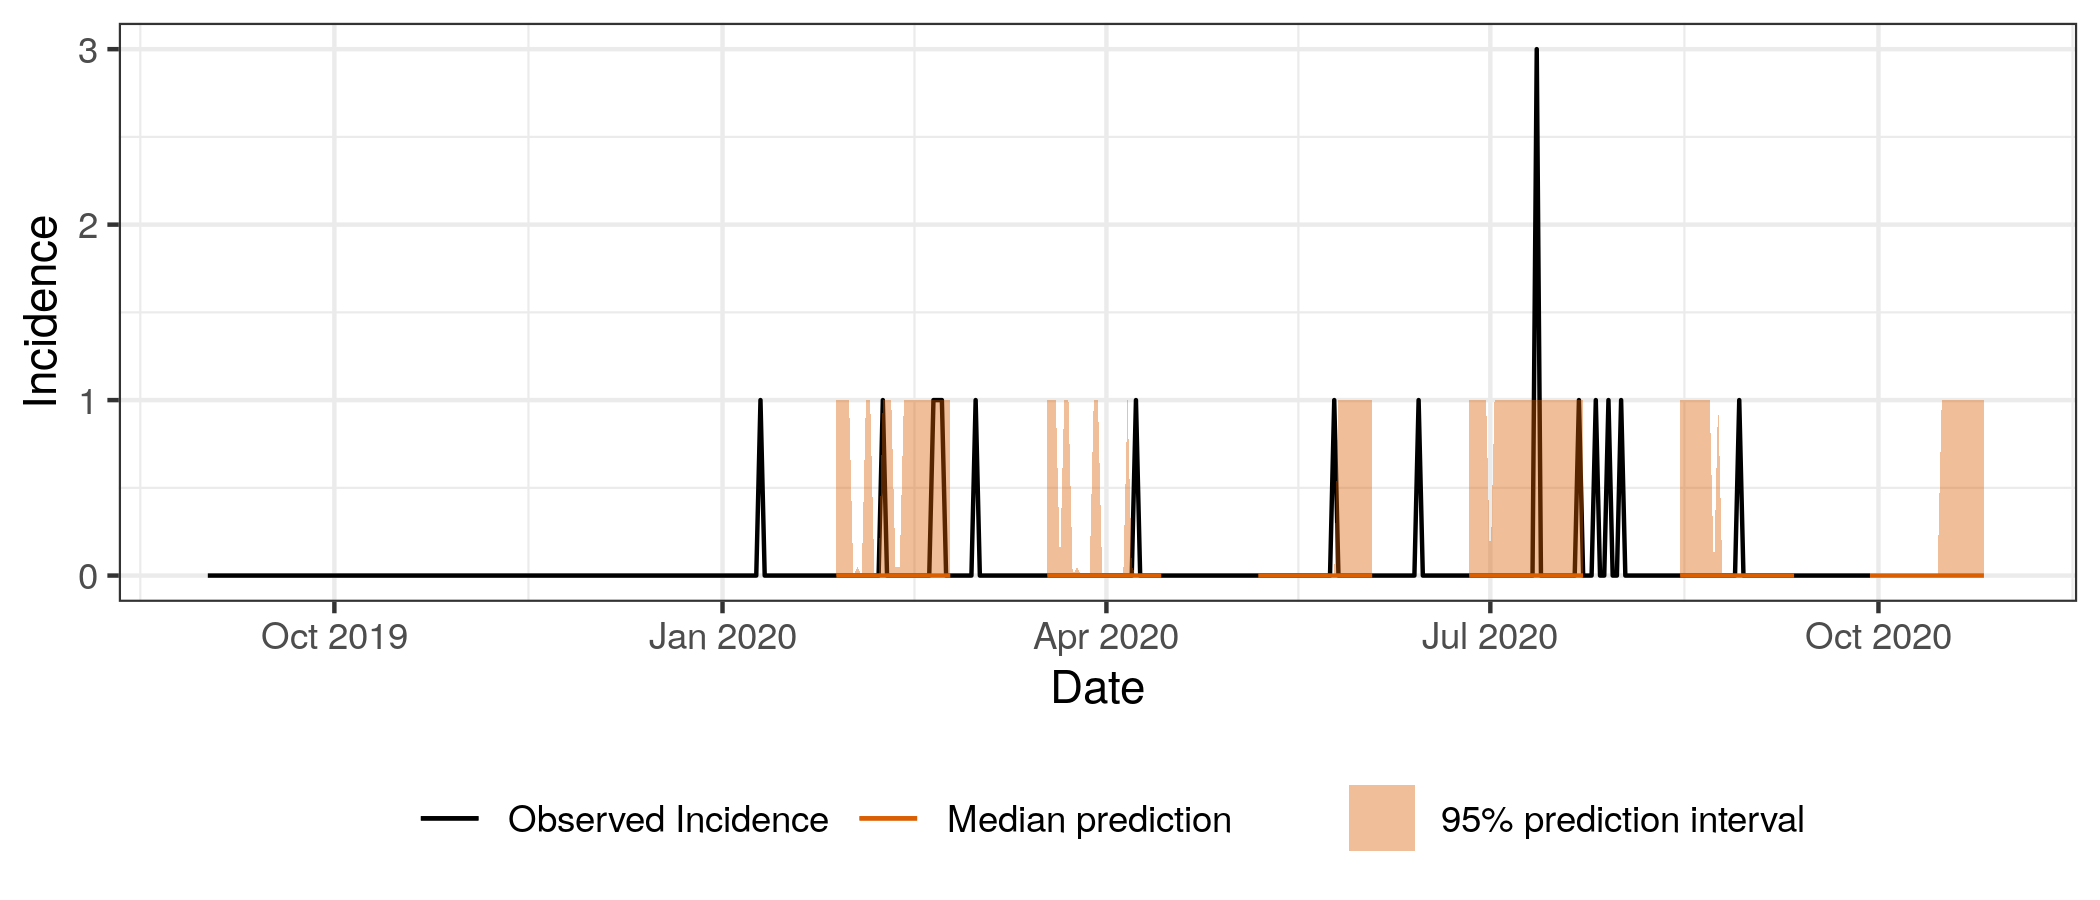
\includegraphics[width=0.9\linewidth, height=7cm]{../output/Biena_predictions.png}  \caption{Forecasted and predicted incidence for the semilocal poisson model}\end{subfigure}

\begin{subfigure}{\textwidth}  \centering  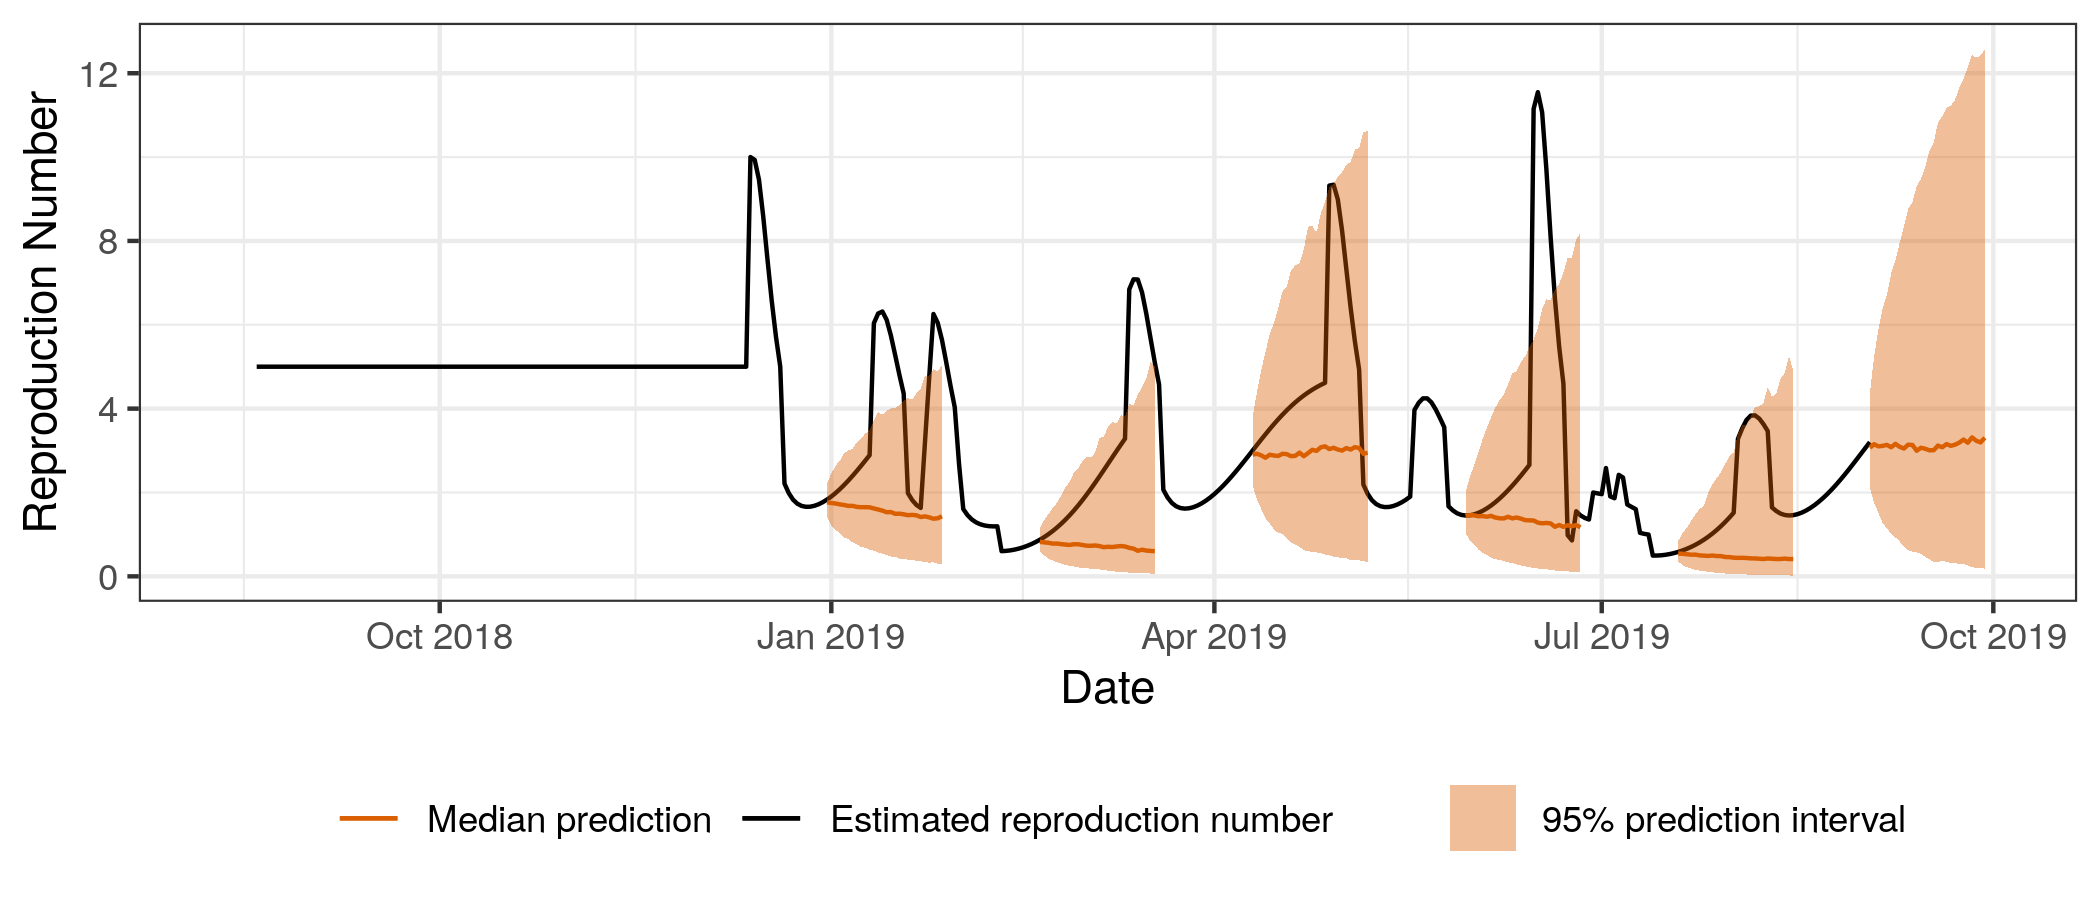
\includegraphics[width=0.9\linewidth, height=7cm]{../output/Biena_Rs.png}  \caption{Forecasted and predicted repreoduction numbers for the semilocal poisson model}\end{subfigure}  \caption{Median forecast with 95 \% prediction intervals and observed values for incidence and reproduction number for the semilocal poisson model for Biena.}\end{figure}

\begin{figure}[H]
\begin{subfigure}{0.5\textwidth}
  \centering
  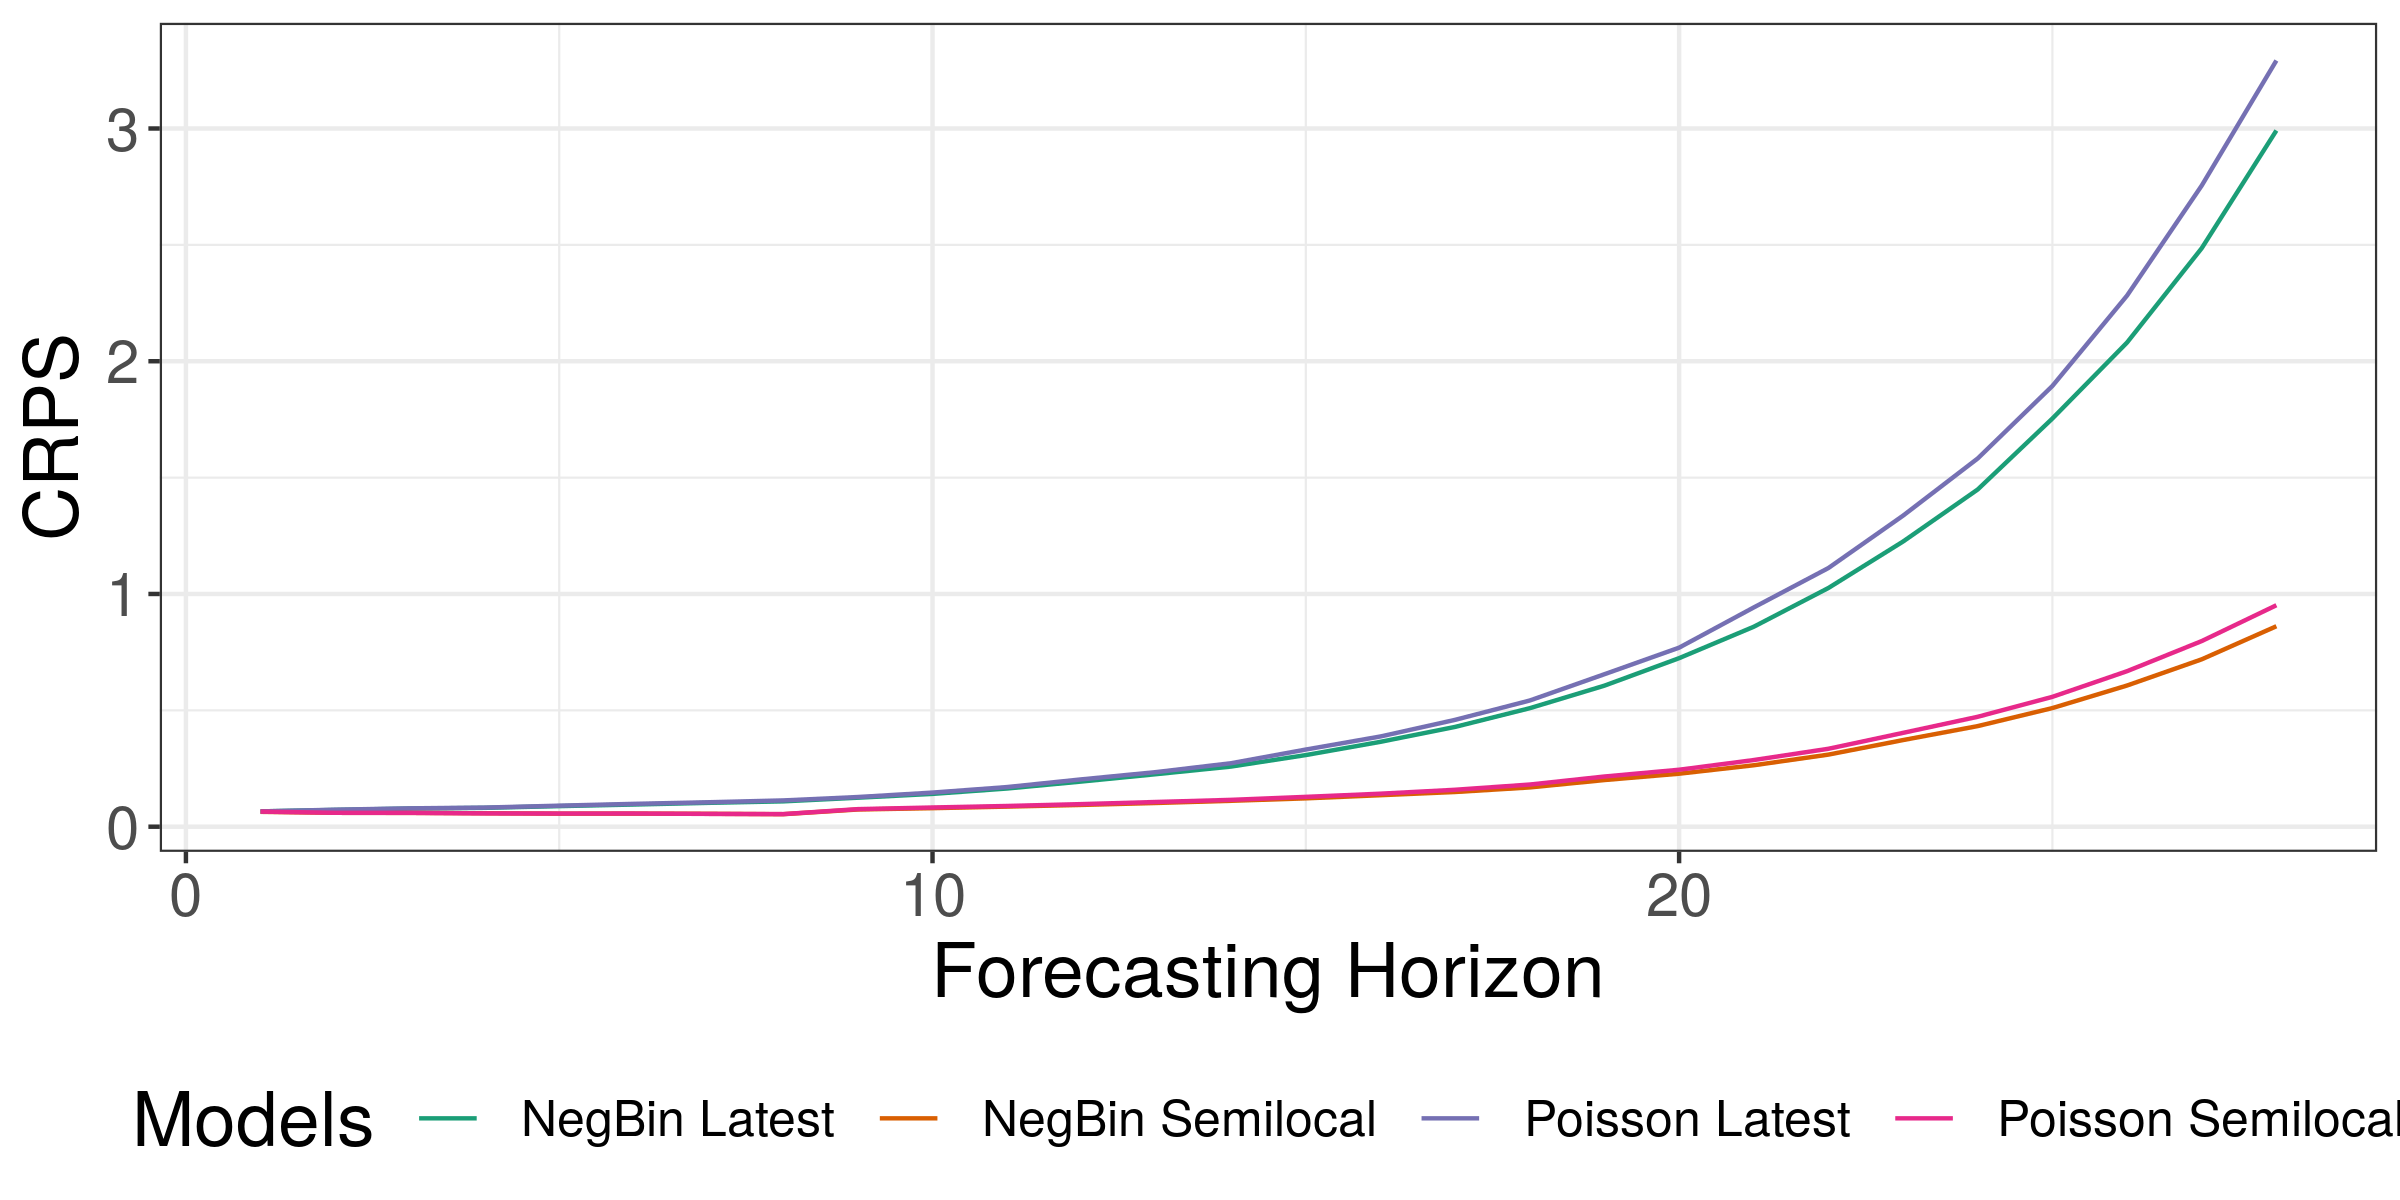
\includegraphics[width=\linewidth]{../output/Biena_crps.png}  
  \caption{Contineously Ranked Probability Score}
  \label{fig:sub-first}
\end{subfigure}
\begin{subfigure}{0.5\textwidth}
  \centering
  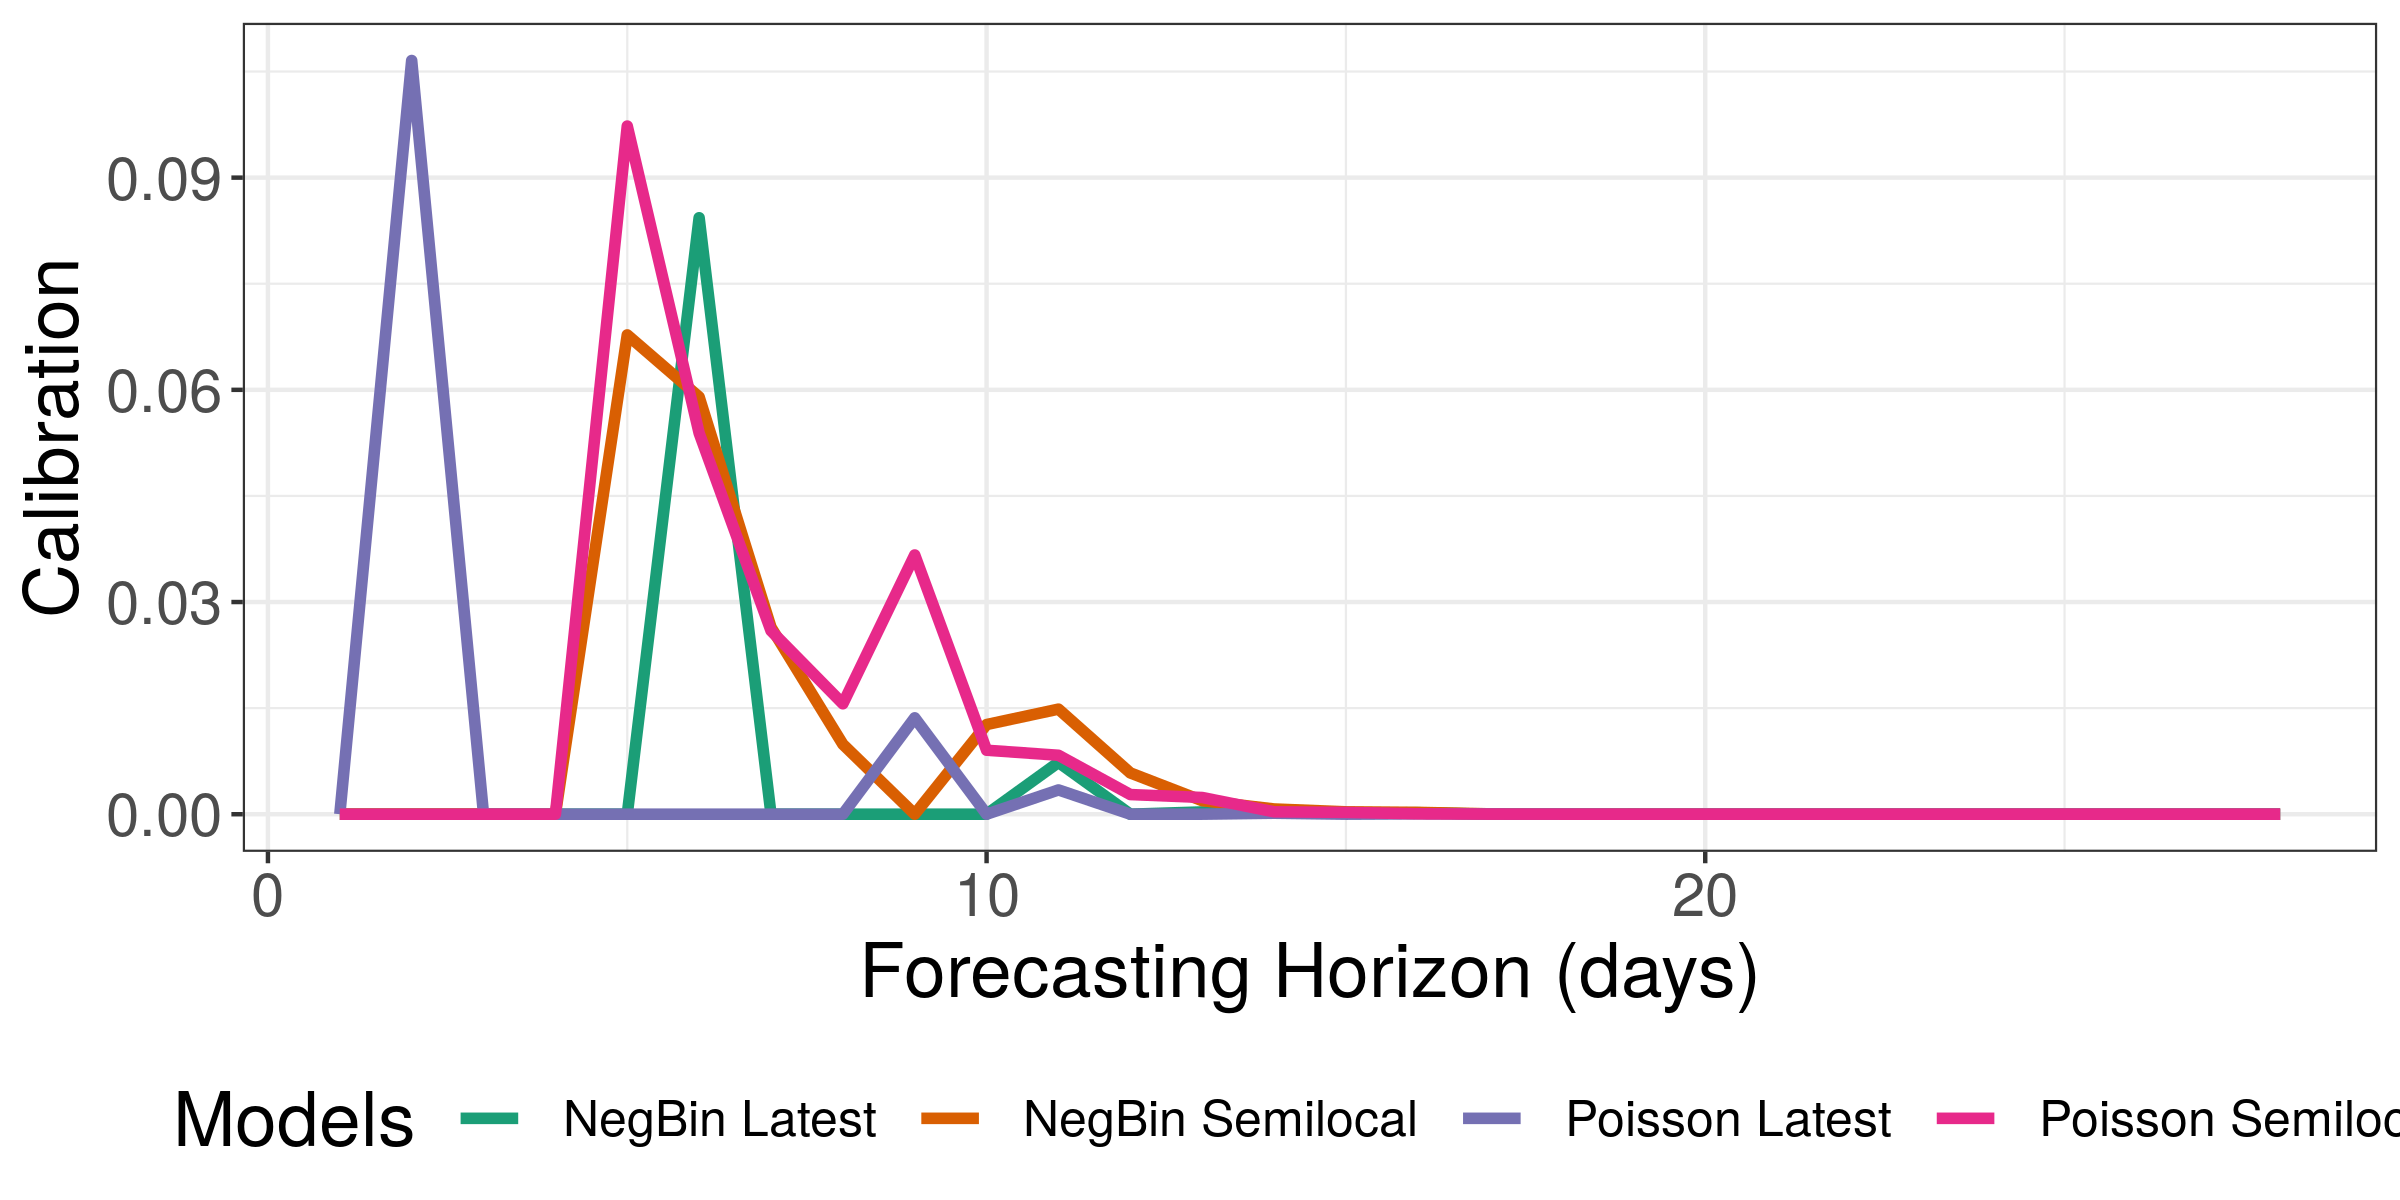
\includegraphics[width=\linewidth]{../output/Biena_calibration.png}  
  \caption{Calibration p-value}
  \label{fig:sub-second}
\end{subfigure}

\begin{subfigure}{0.5\textwidth}
  \centering
  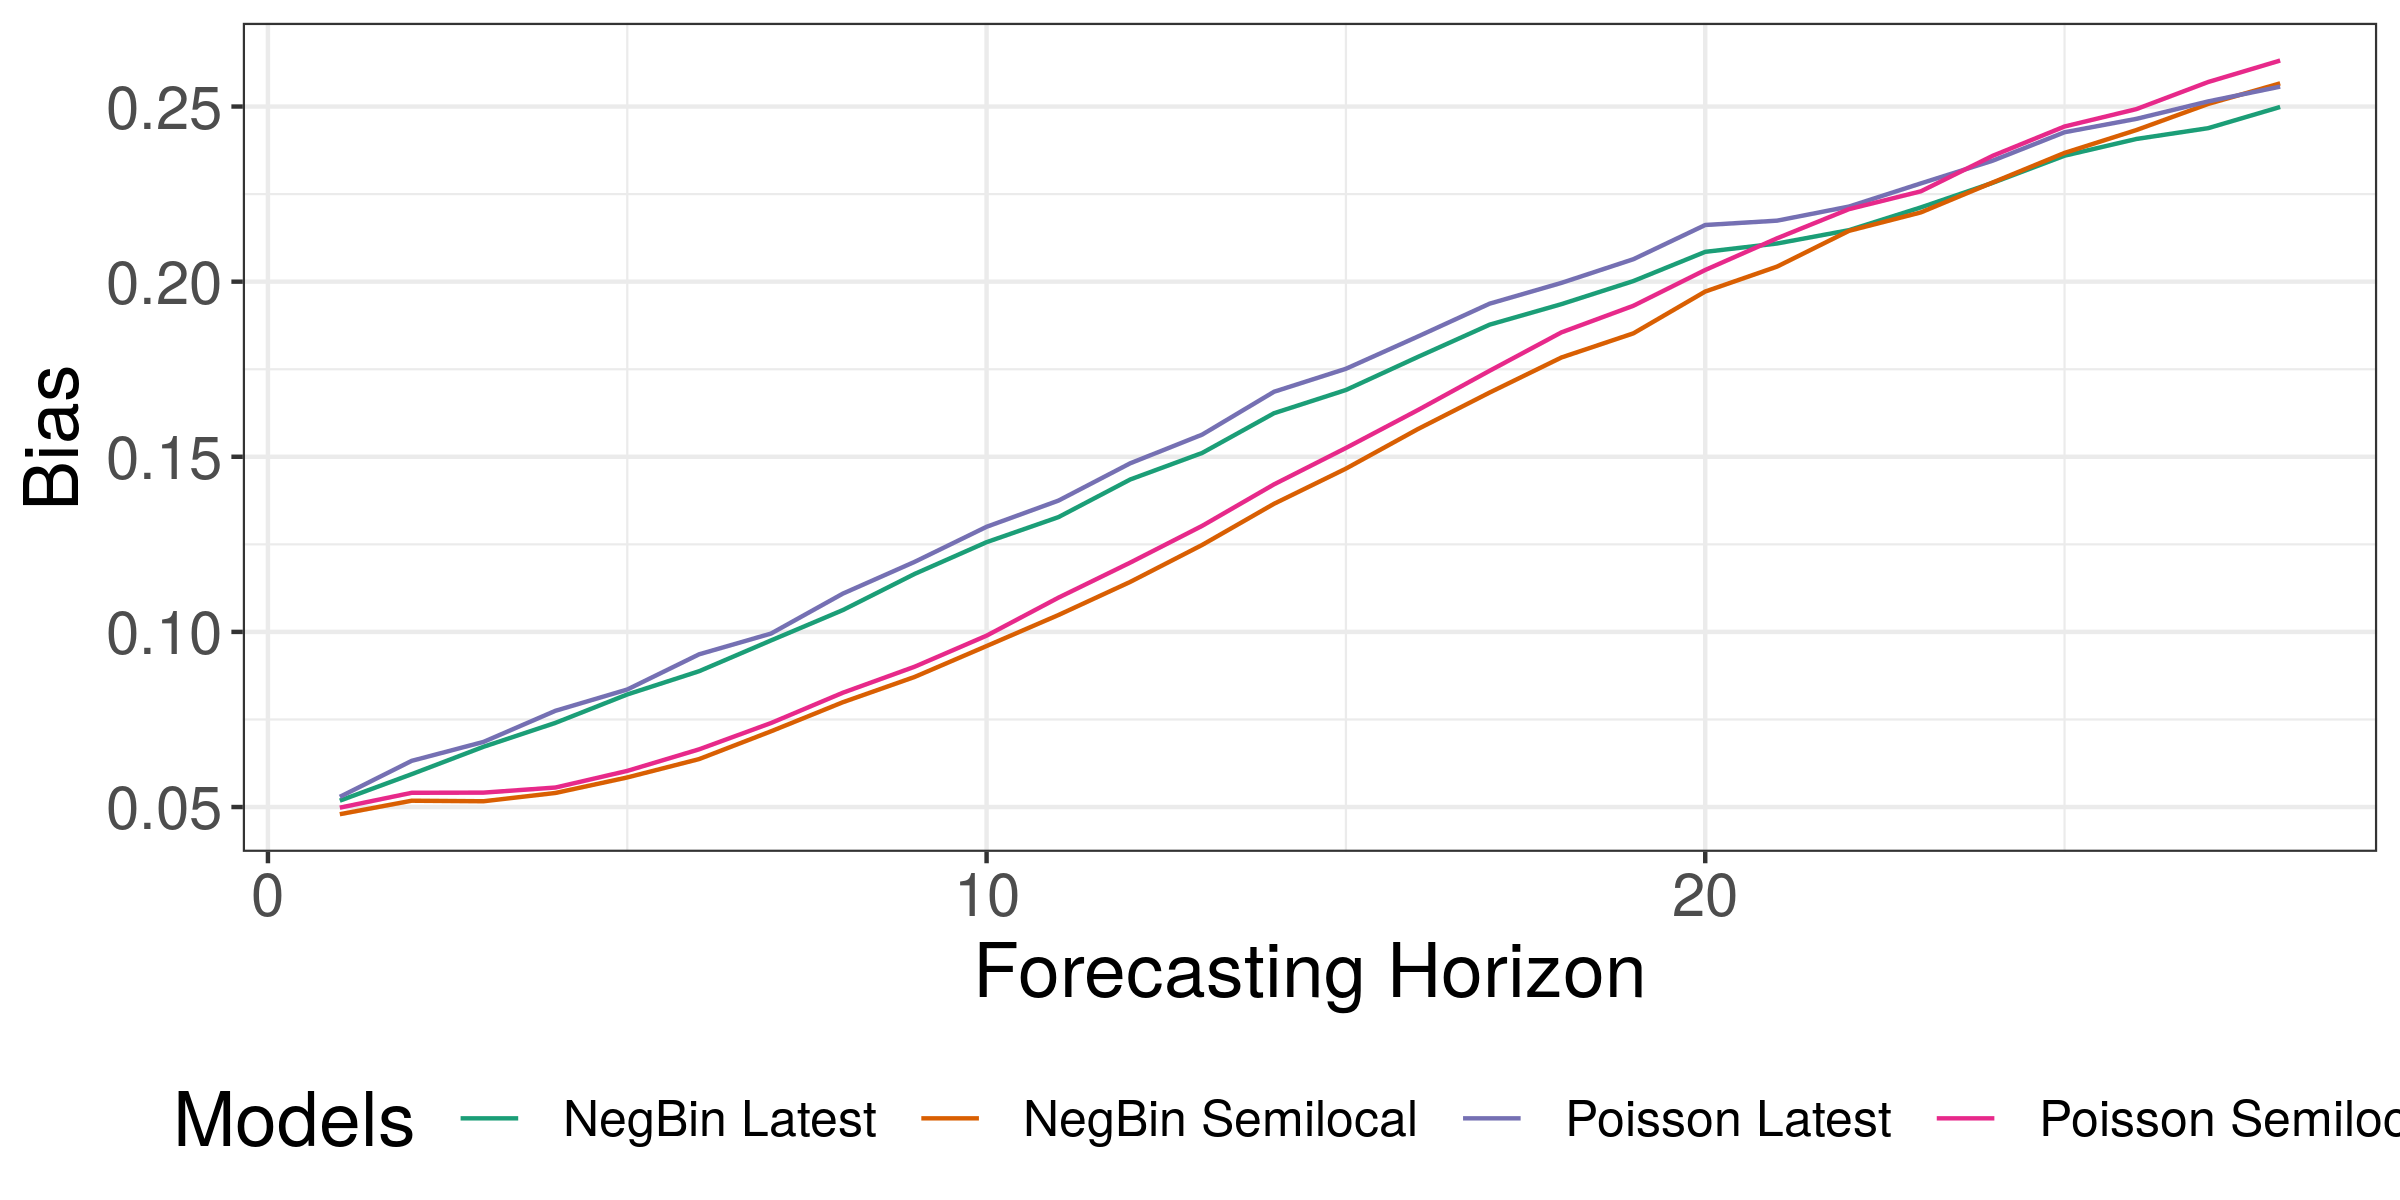
\includegraphics[width=\linewidth]{../output/Biena_bias.png}  
  \caption{Bias}
  \label{fig:sub-third}
\end{subfigure}
\begin{subfigure}{0.5\textwidth}
  \centering
  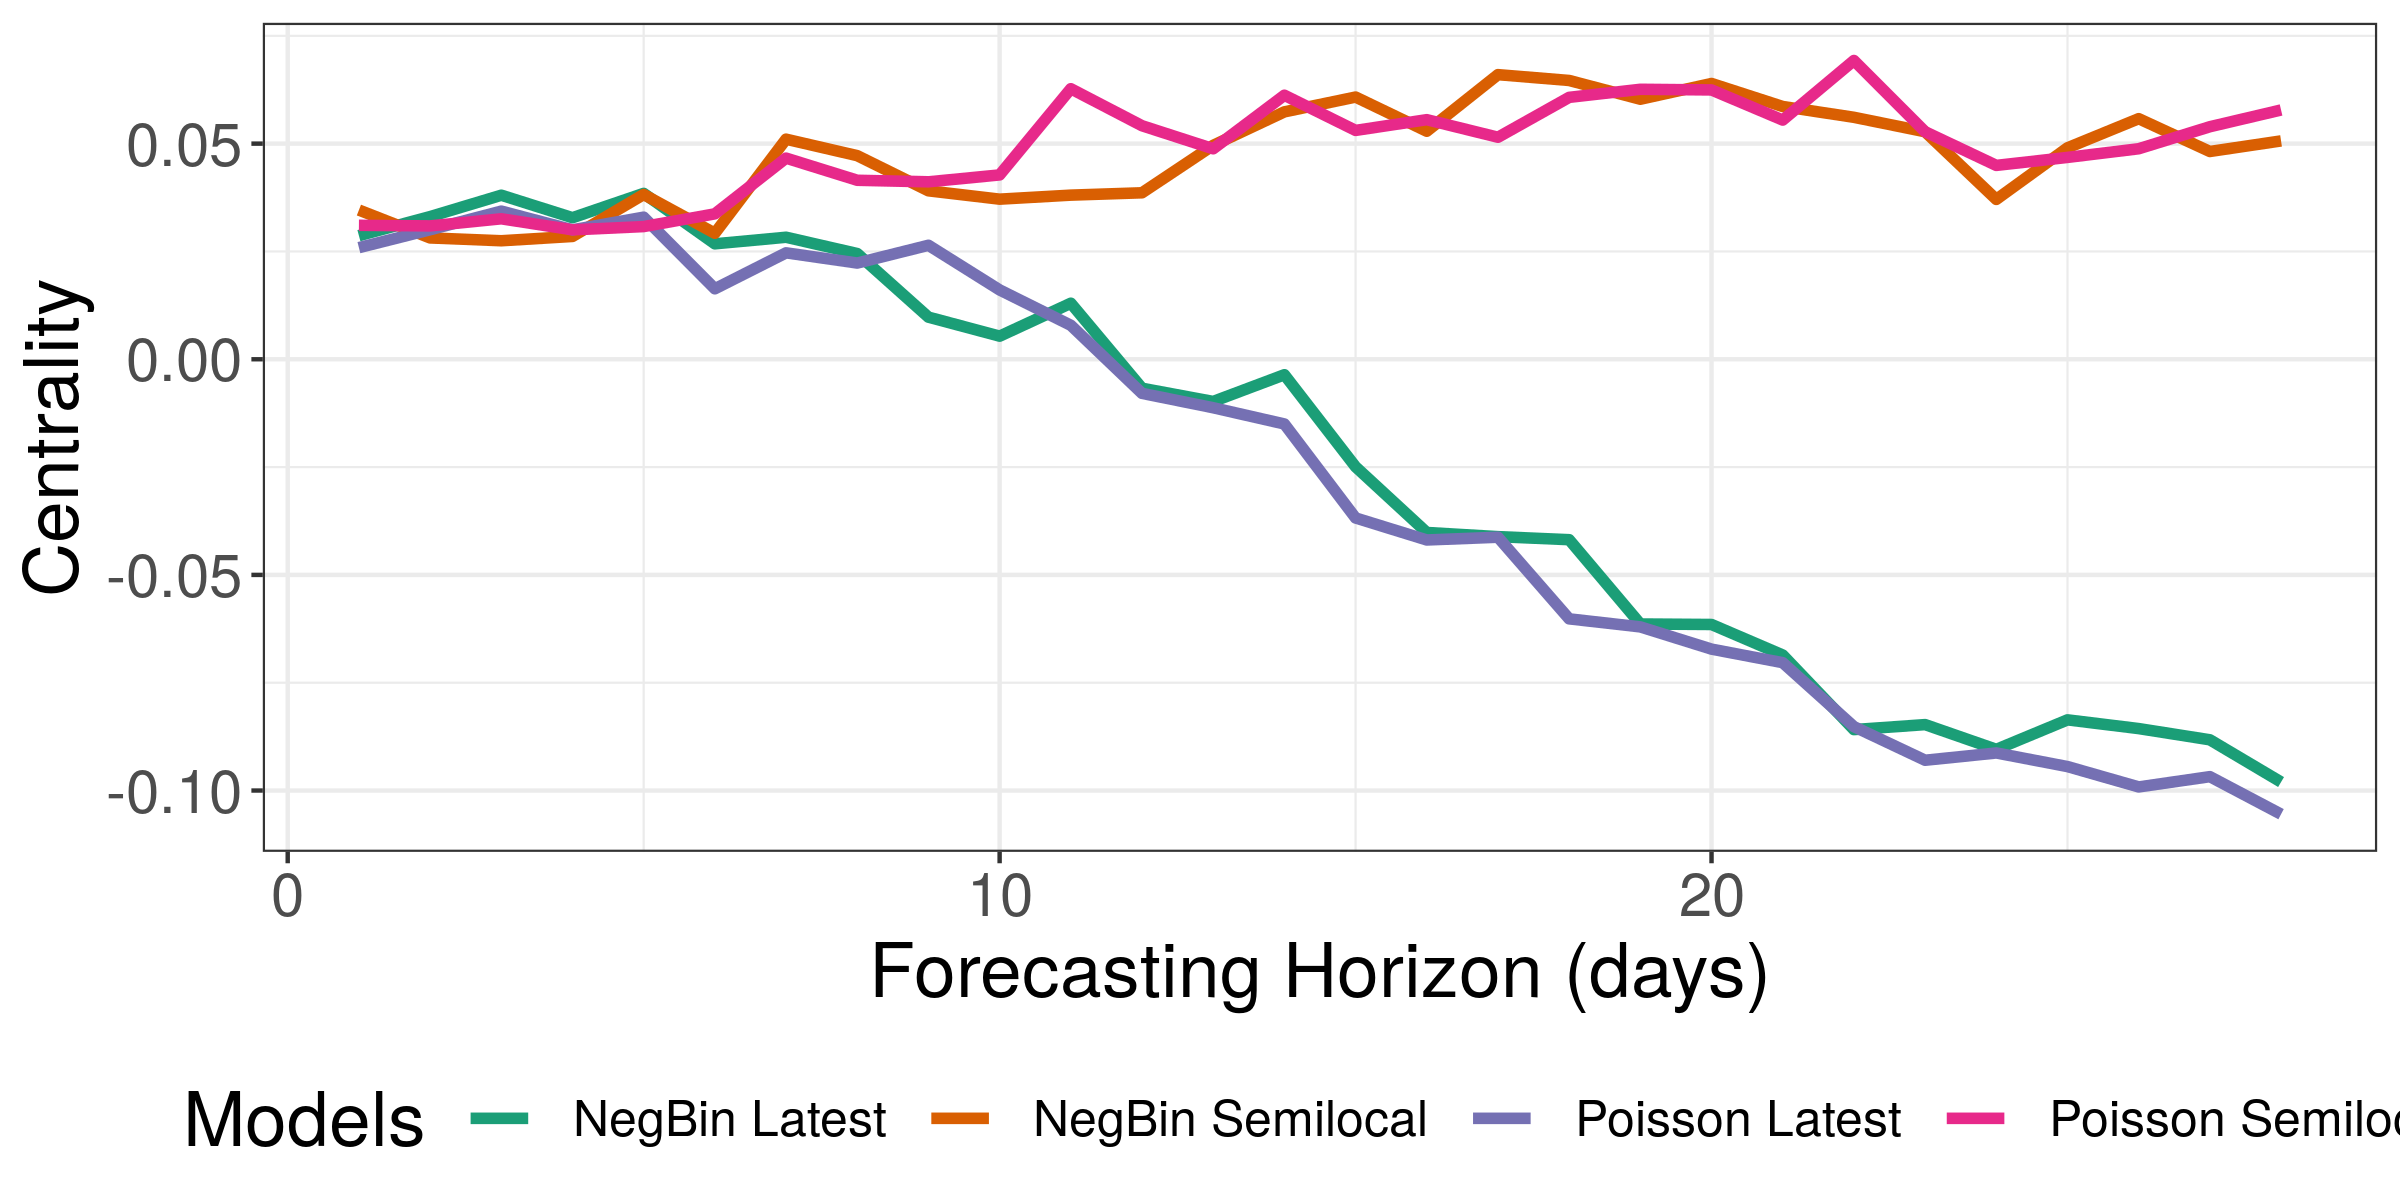
\includegraphics[width=\linewidth]{../output/Biena_centrality.png}  
  \caption{Centrality of PIT values}
  \label{fig:nat_scores_4}
\end{subfigure}
  \caption{Scores for the entire outbreak as a function of the forecasting horizon.}

  \label{fig:nat_scores}
\end{figure}
 \section{ Bunia }\begin{figure}[H]\begin{subfigure}{\textwidth}  \centering  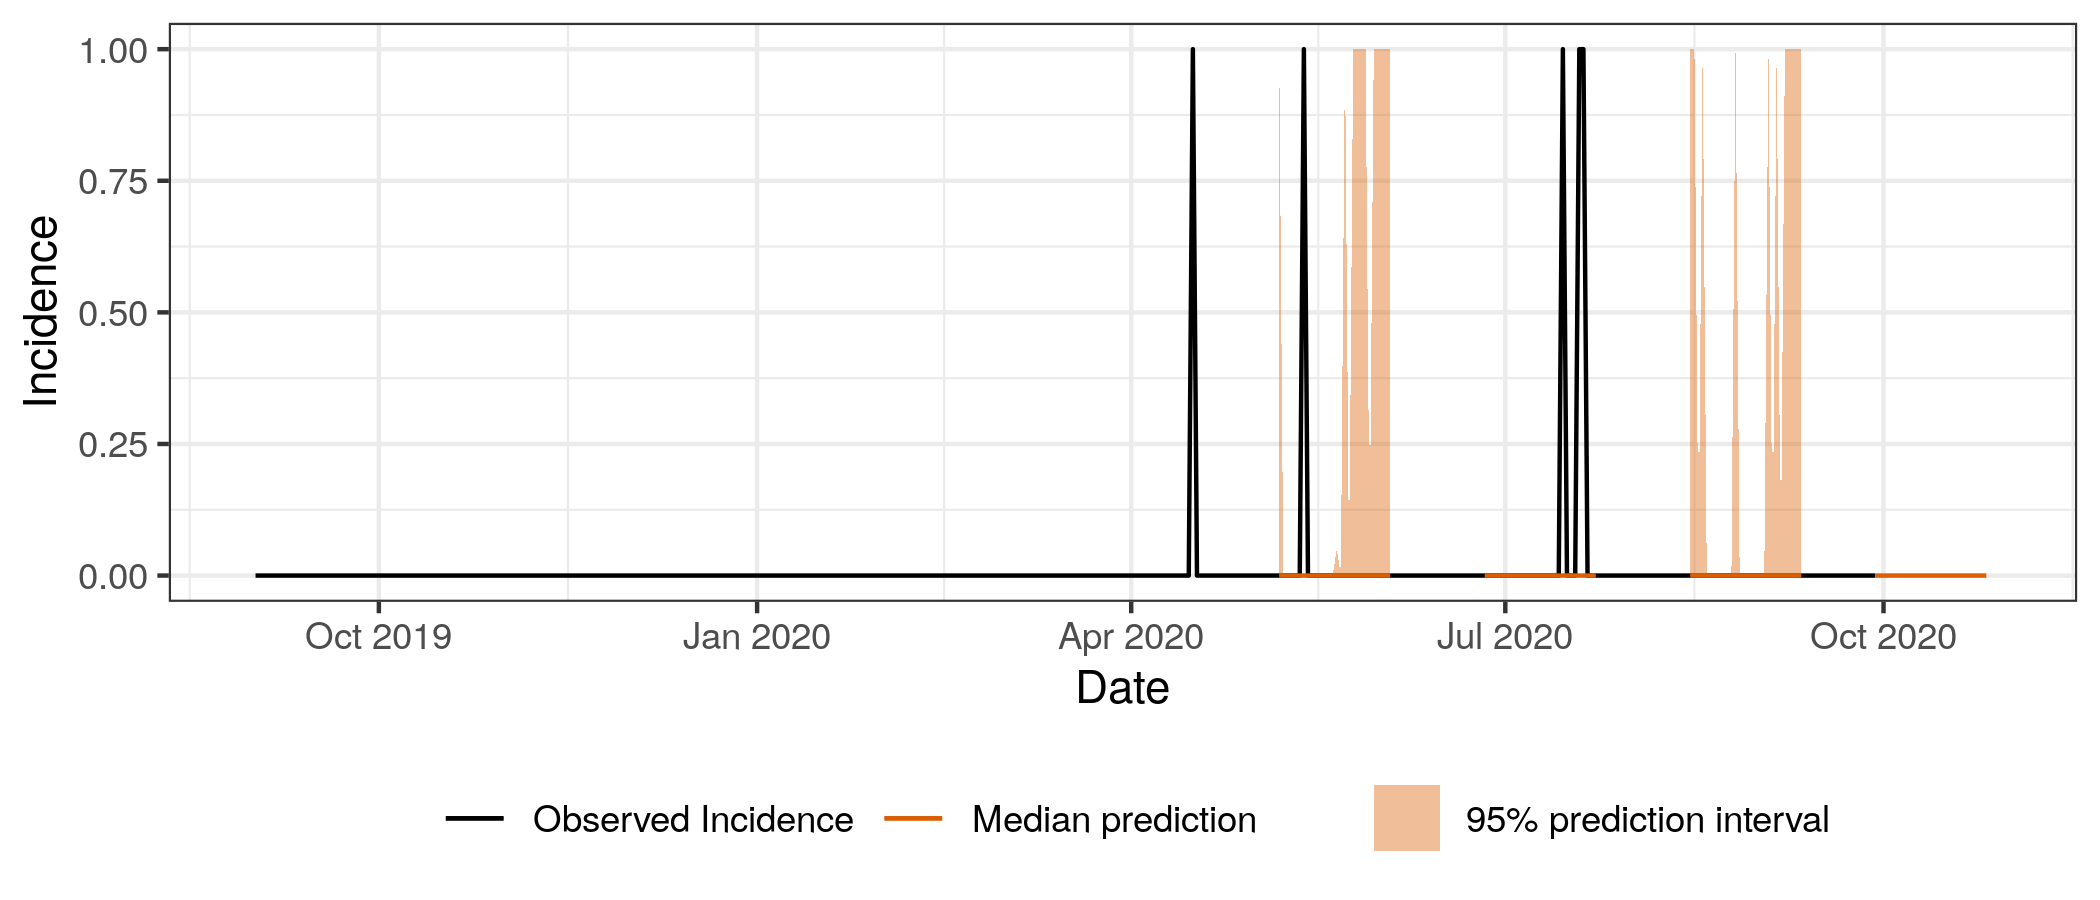
\includegraphics[width=0.9\linewidth, height=7cm]{../output/Bunia_predictions.png}  \caption{Forecasted and predicted incidence for the semilocal poisson model}\end{subfigure}

\begin{subfigure}{\textwidth}  \centering  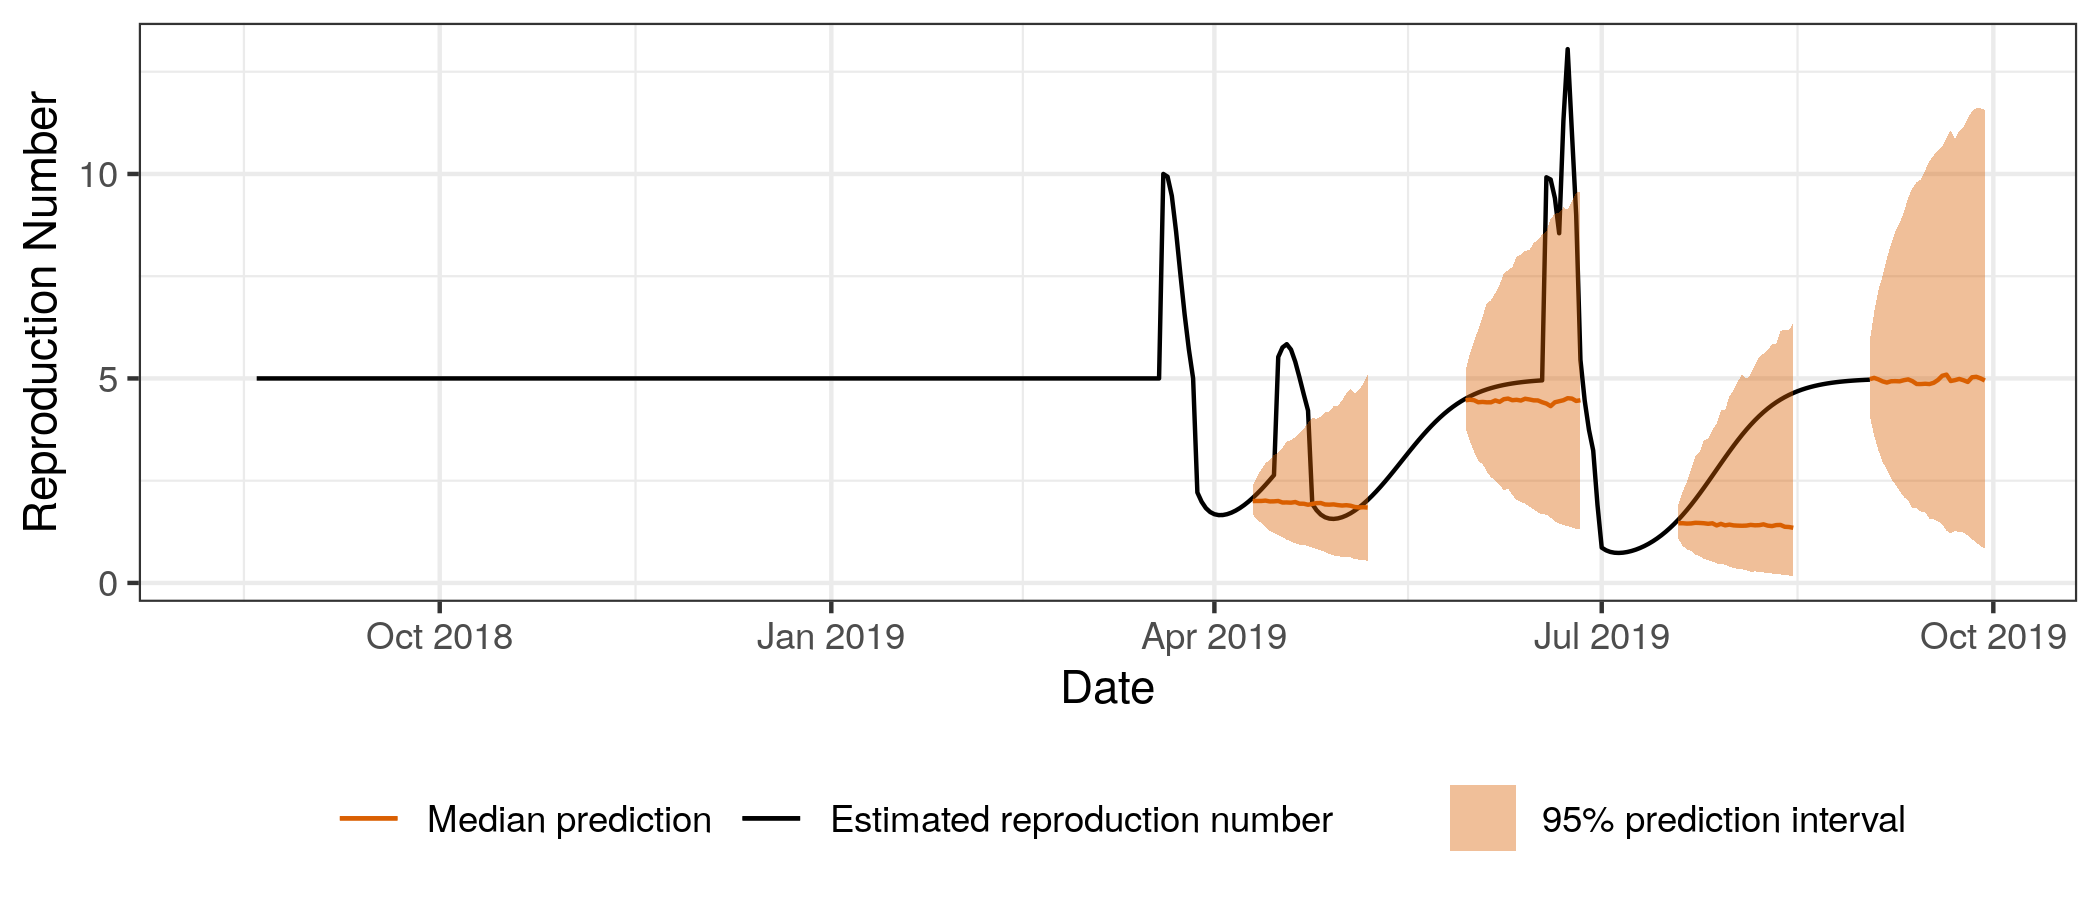
\includegraphics[width=0.9\linewidth, height=7cm]{../output/Bunia_Rs.png}  \caption{Forecasted and predicted repreoduction numbers for the semilocal poisson model}\end{subfigure}  \caption{Median forecast with 95 \% prediction intervals and observed values for incidence and reproduction number for the semilocal poisson model for Bunia.}\end{figure}

\begin{figure}[H]
\begin{subfigure}{0.5\textwidth}
  \centering
  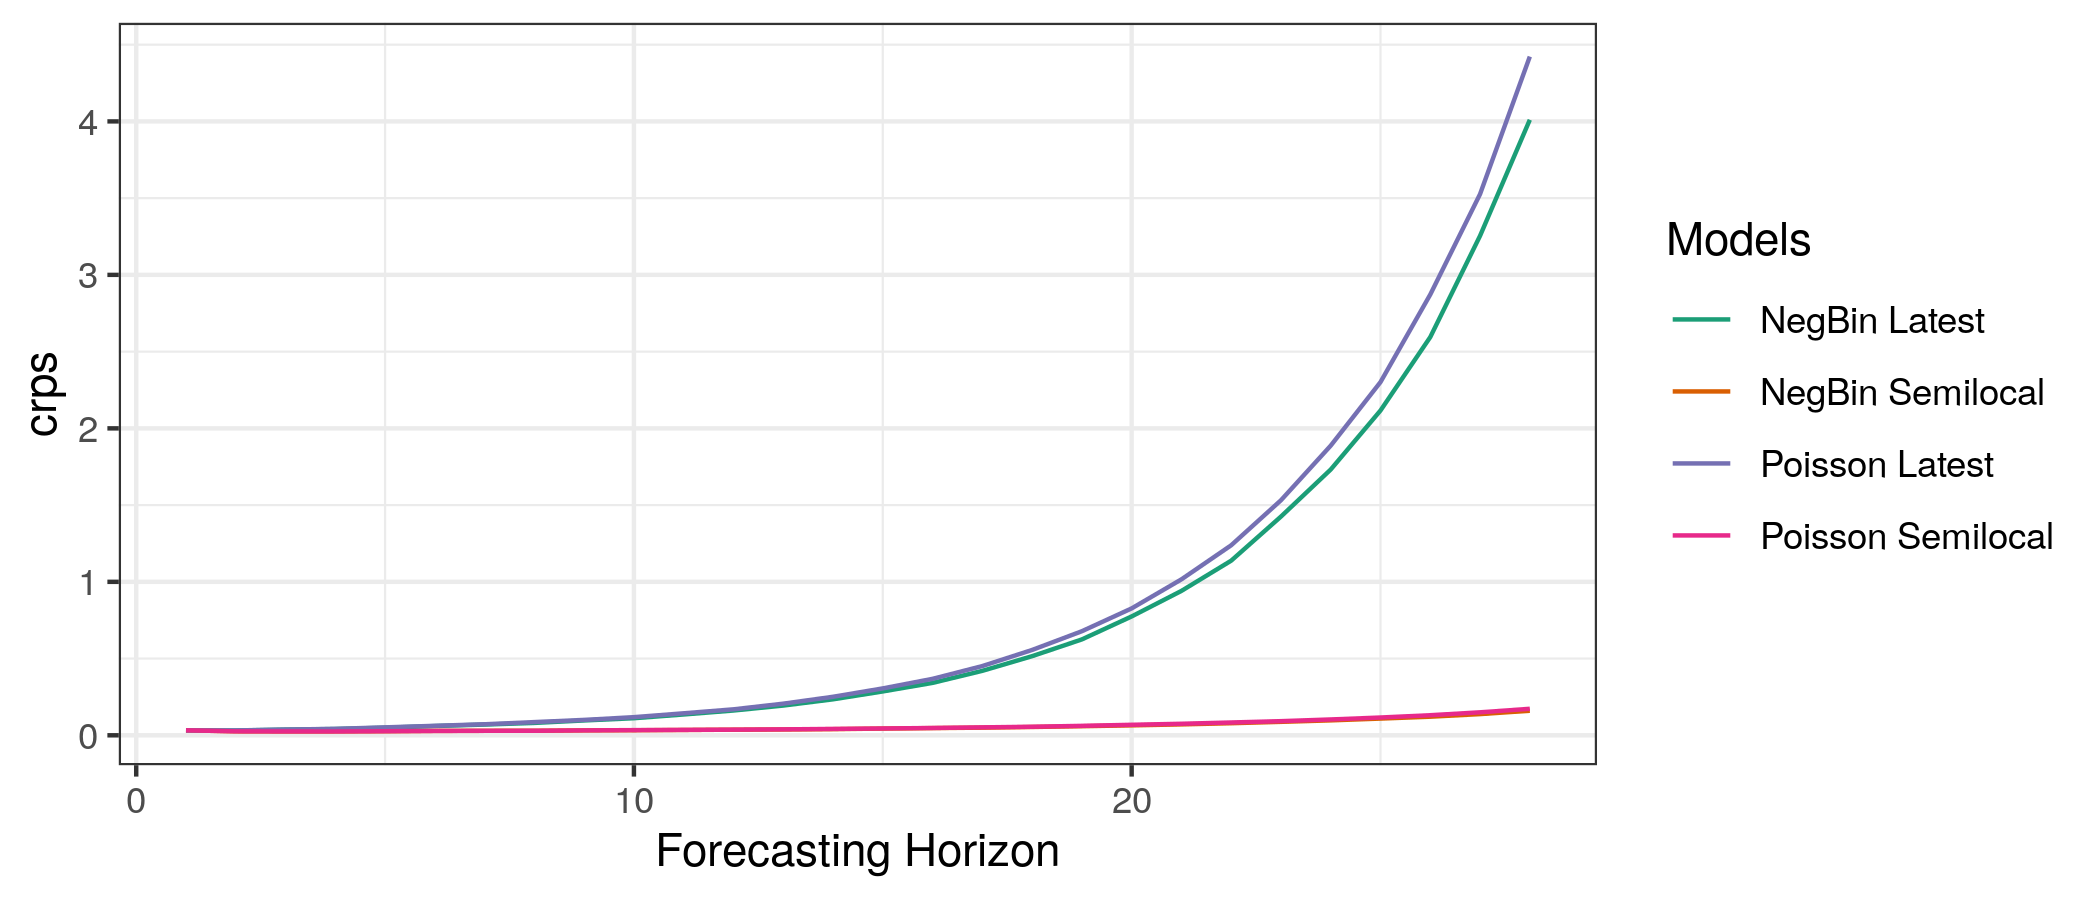
\includegraphics[width=\linewidth]{../output/Bunia_crps.png}  
  \caption{Contineously Ranked Probability Score}
  \label{fig:sub-first}
\end{subfigure}
\begin{subfigure}{0.5\textwidth}
  \centering
  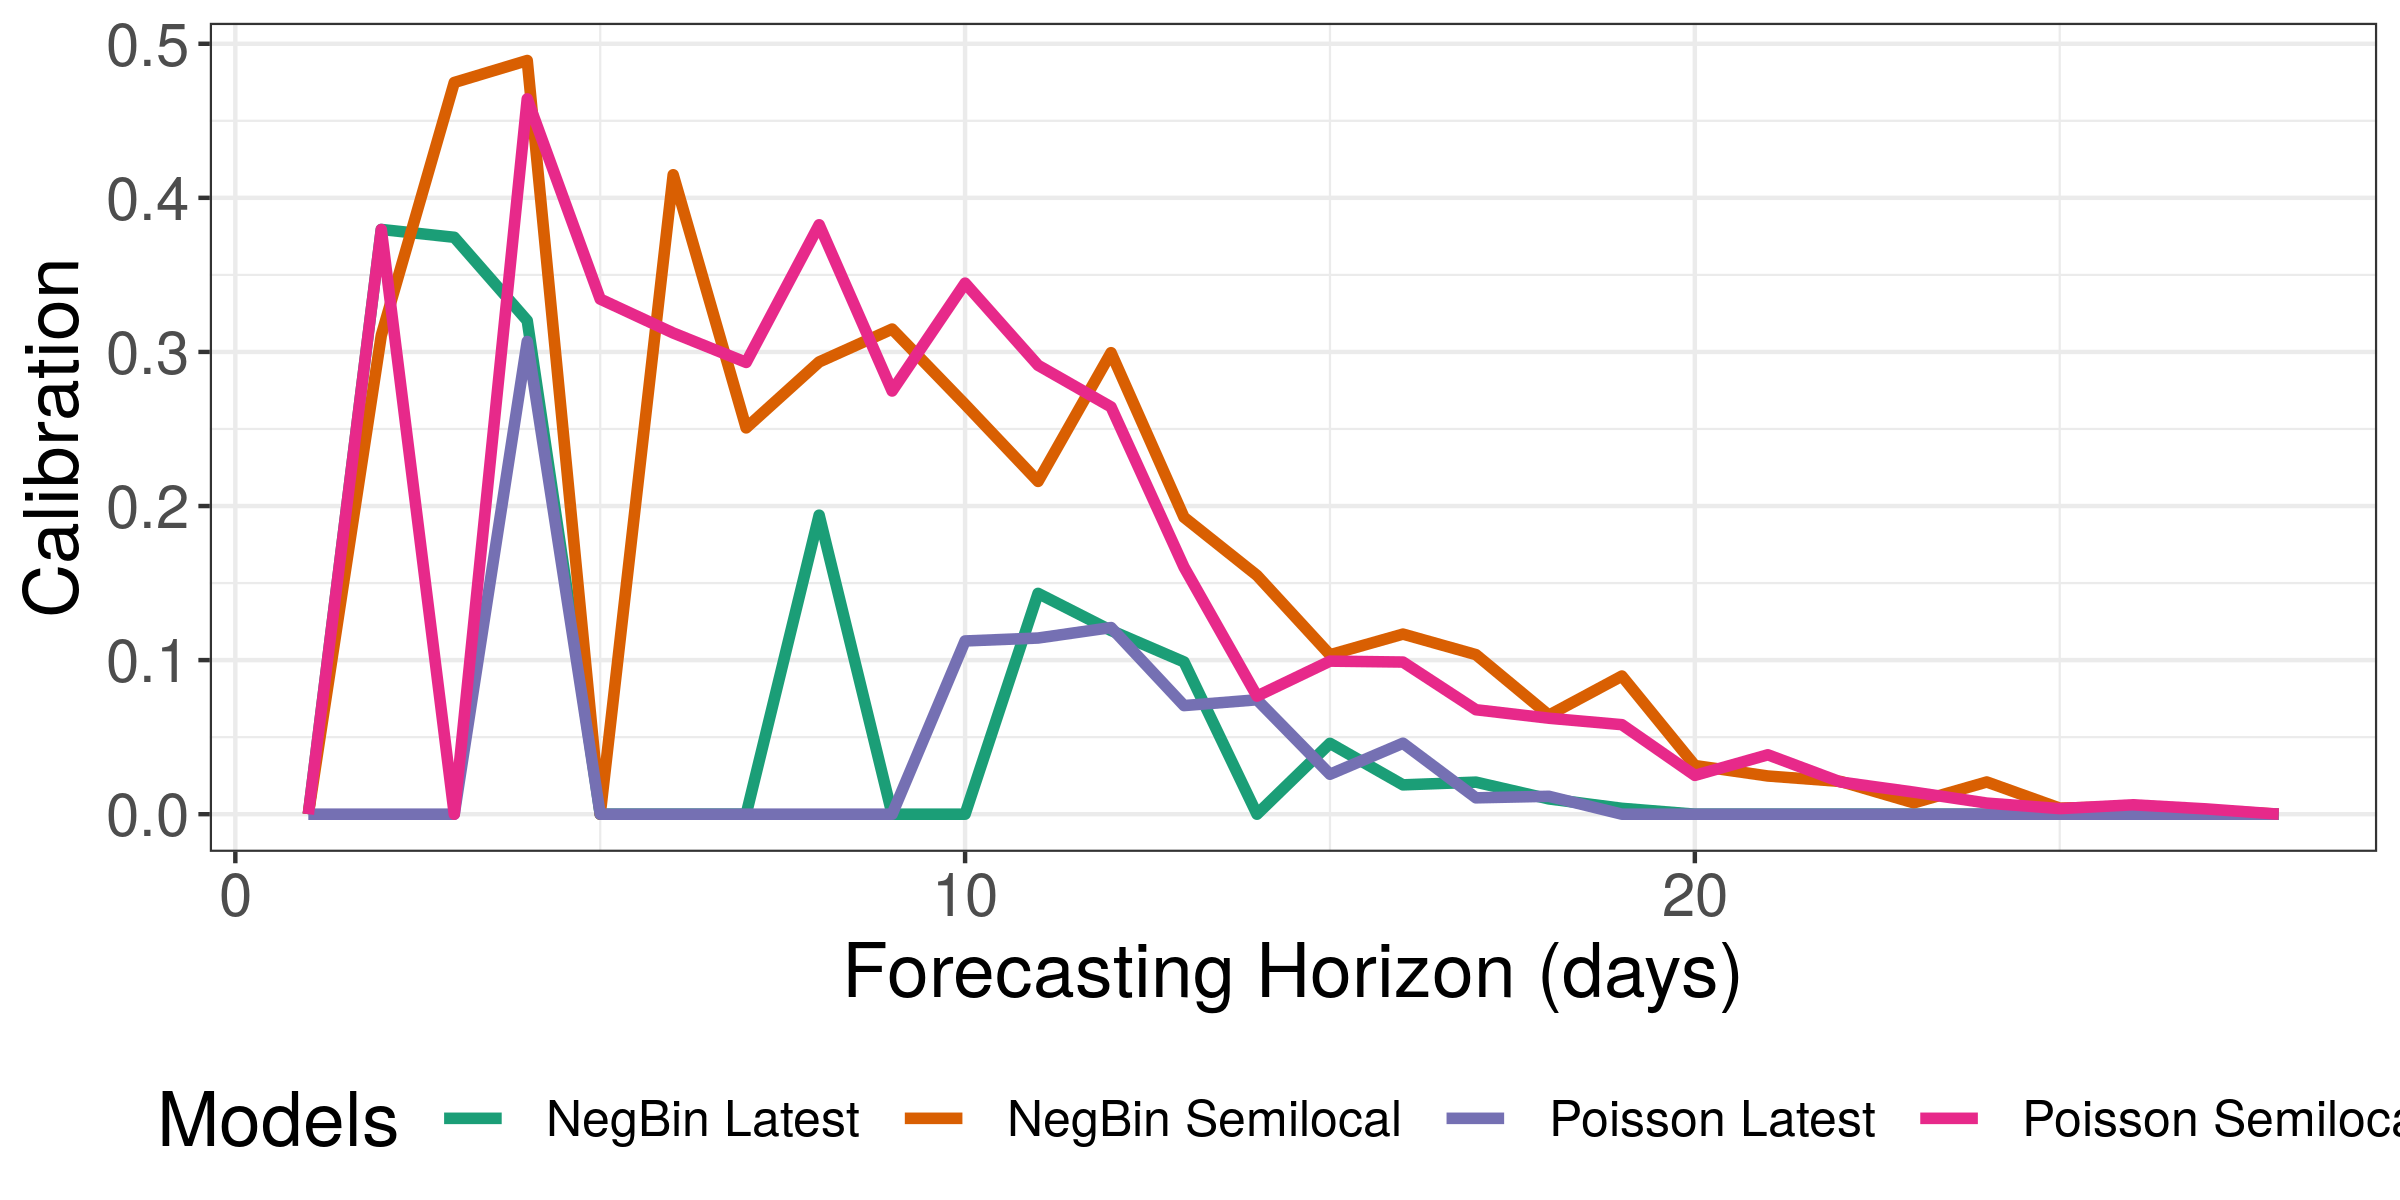
\includegraphics[width=\linewidth]{../output/Bunia_calibration.png}  
  \caption{Calibration p-value}
  \label{fig:sub-second}
\end{subfigure}

\begin{subfigure}{0.5\textwidth}
  \centering
  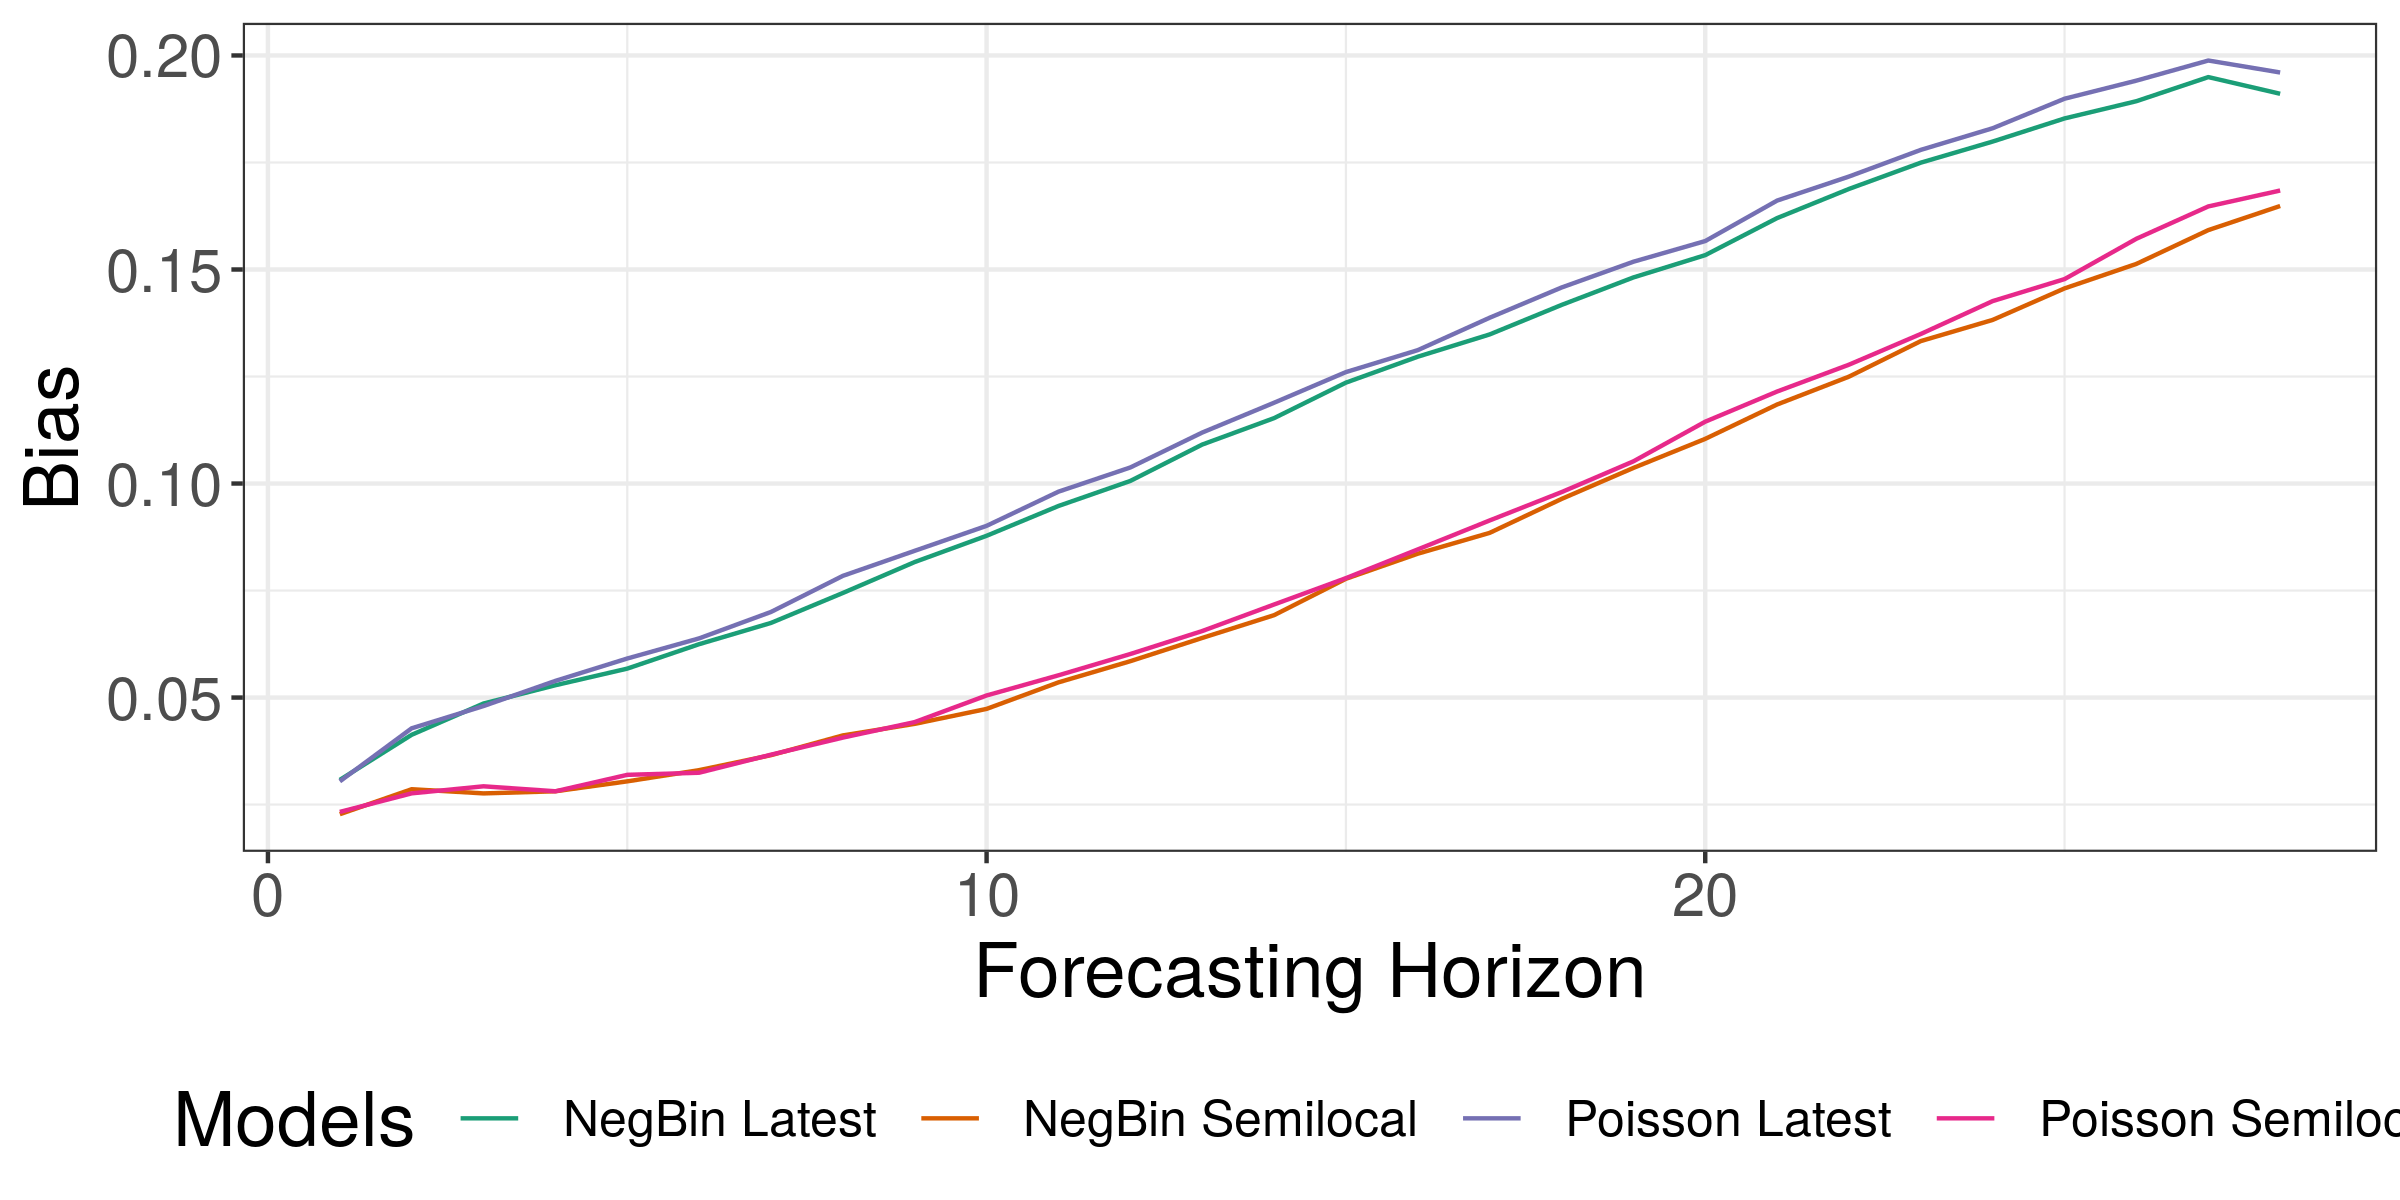
\includegraphics[width=\linewidth]{../output/Bunia_bias.png}  
  \caption{Bias}
  \label{fig:sub-third}
\end{subfigure}
\begin{subfigure}{0.5\textwidth}
  \centering
  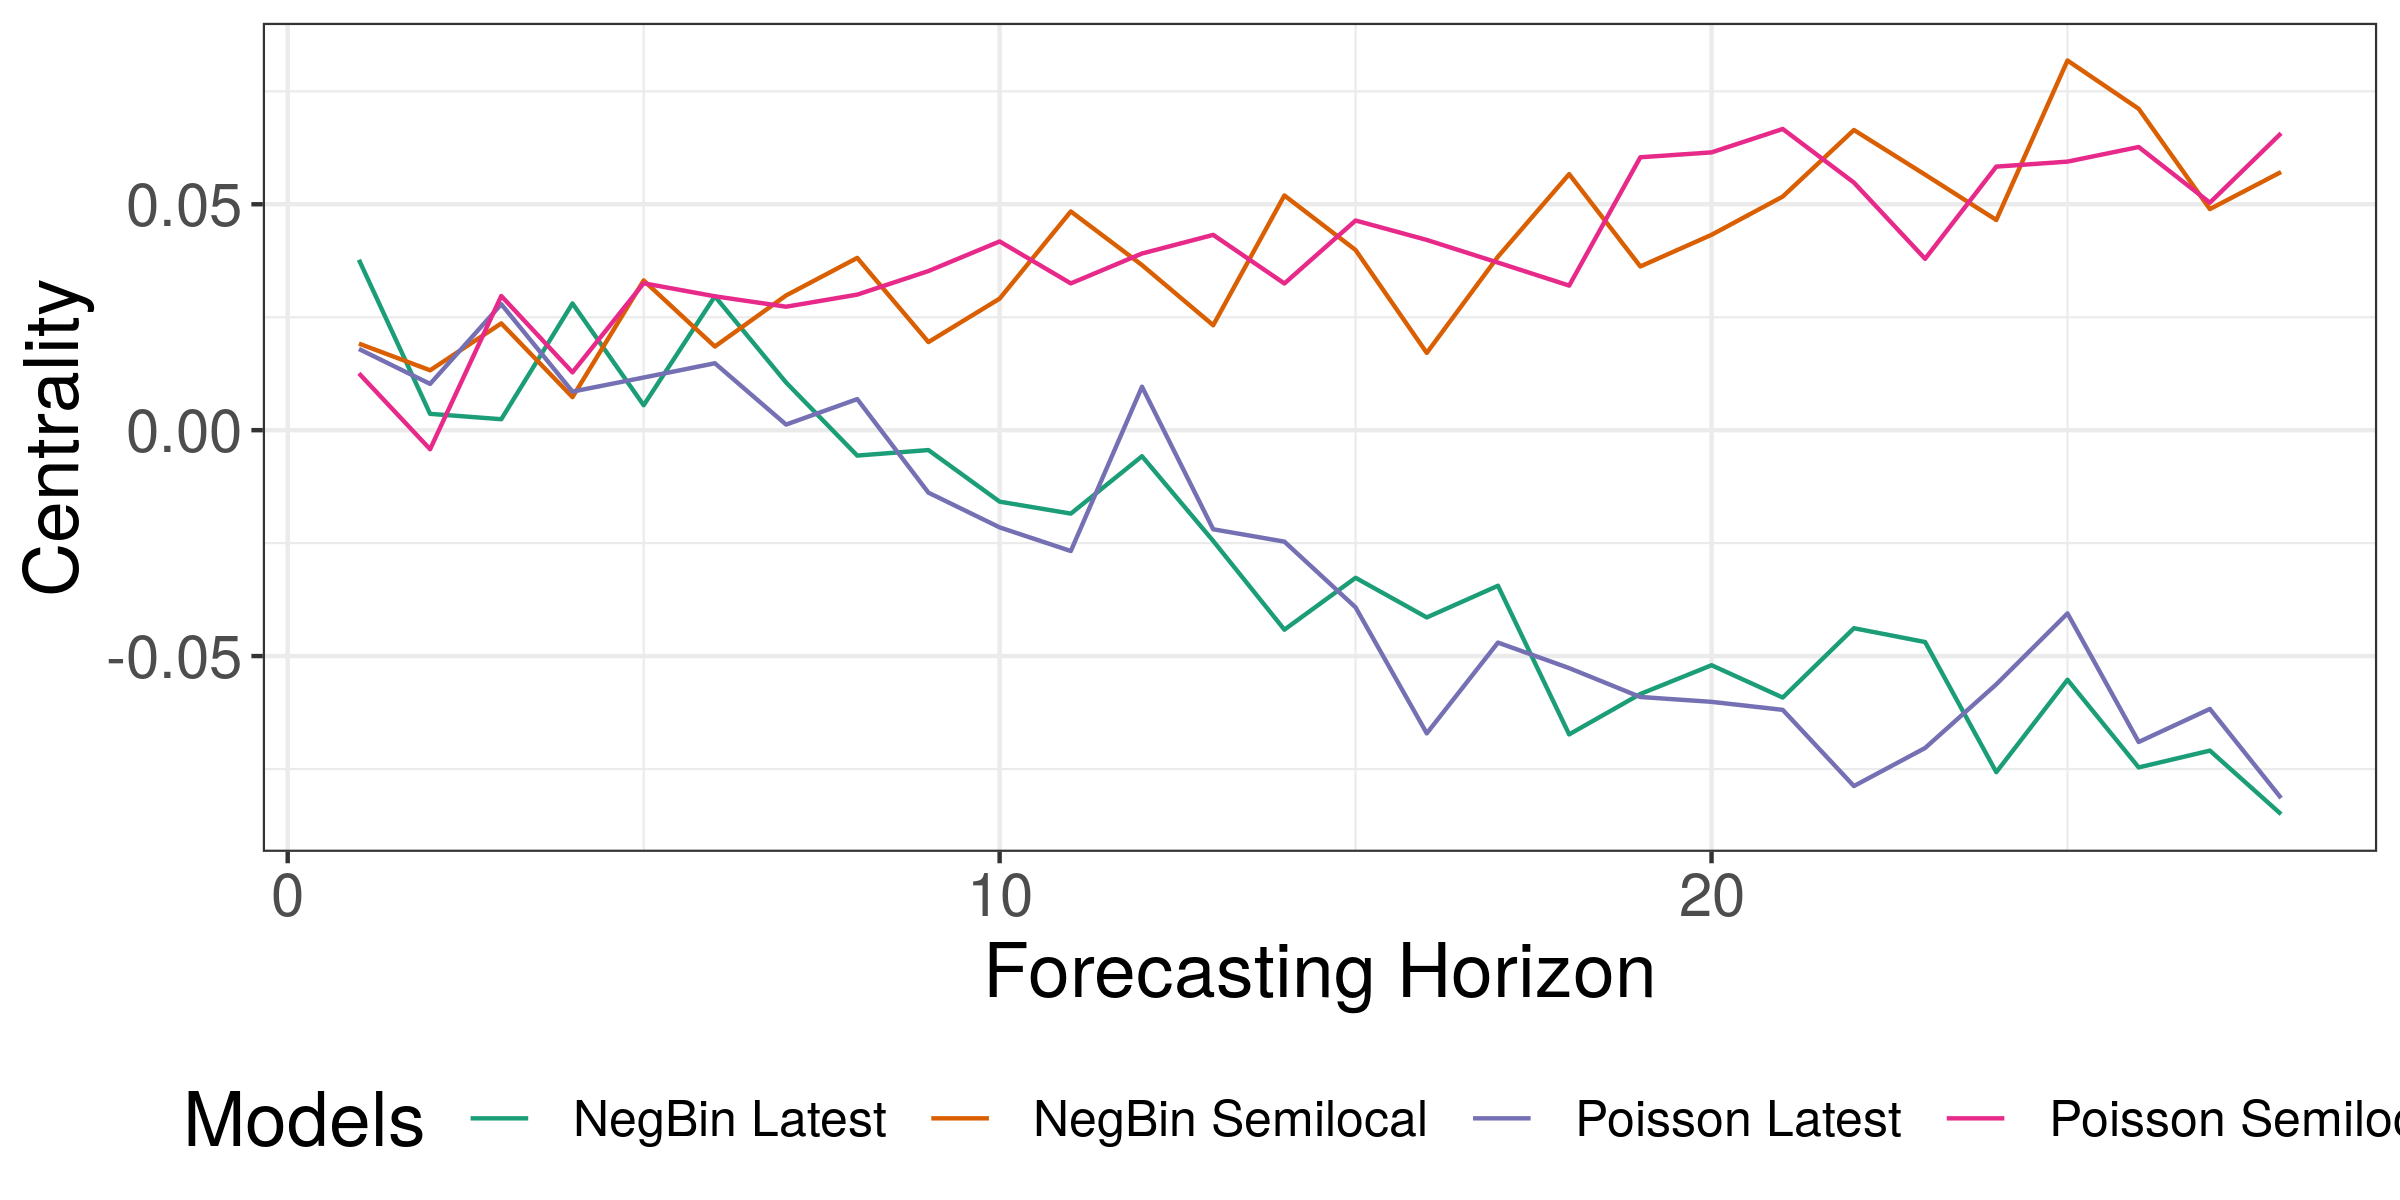
\includegraphics[width=\linewidth]{../output/Bunia_centrality.png}  
  \caption{Centrality of PIT values}
  \label{fig:nat_scores_4}
\end{subfigure}
  \caption{Scores for the entire outbreak as a function of the forecasting horizon.}

  \label{fig:nat_scores}
\end{figure}
 \section{ Butembo }\begin{figure}[H]\begin{subfigure}{\textwidth}  \centering  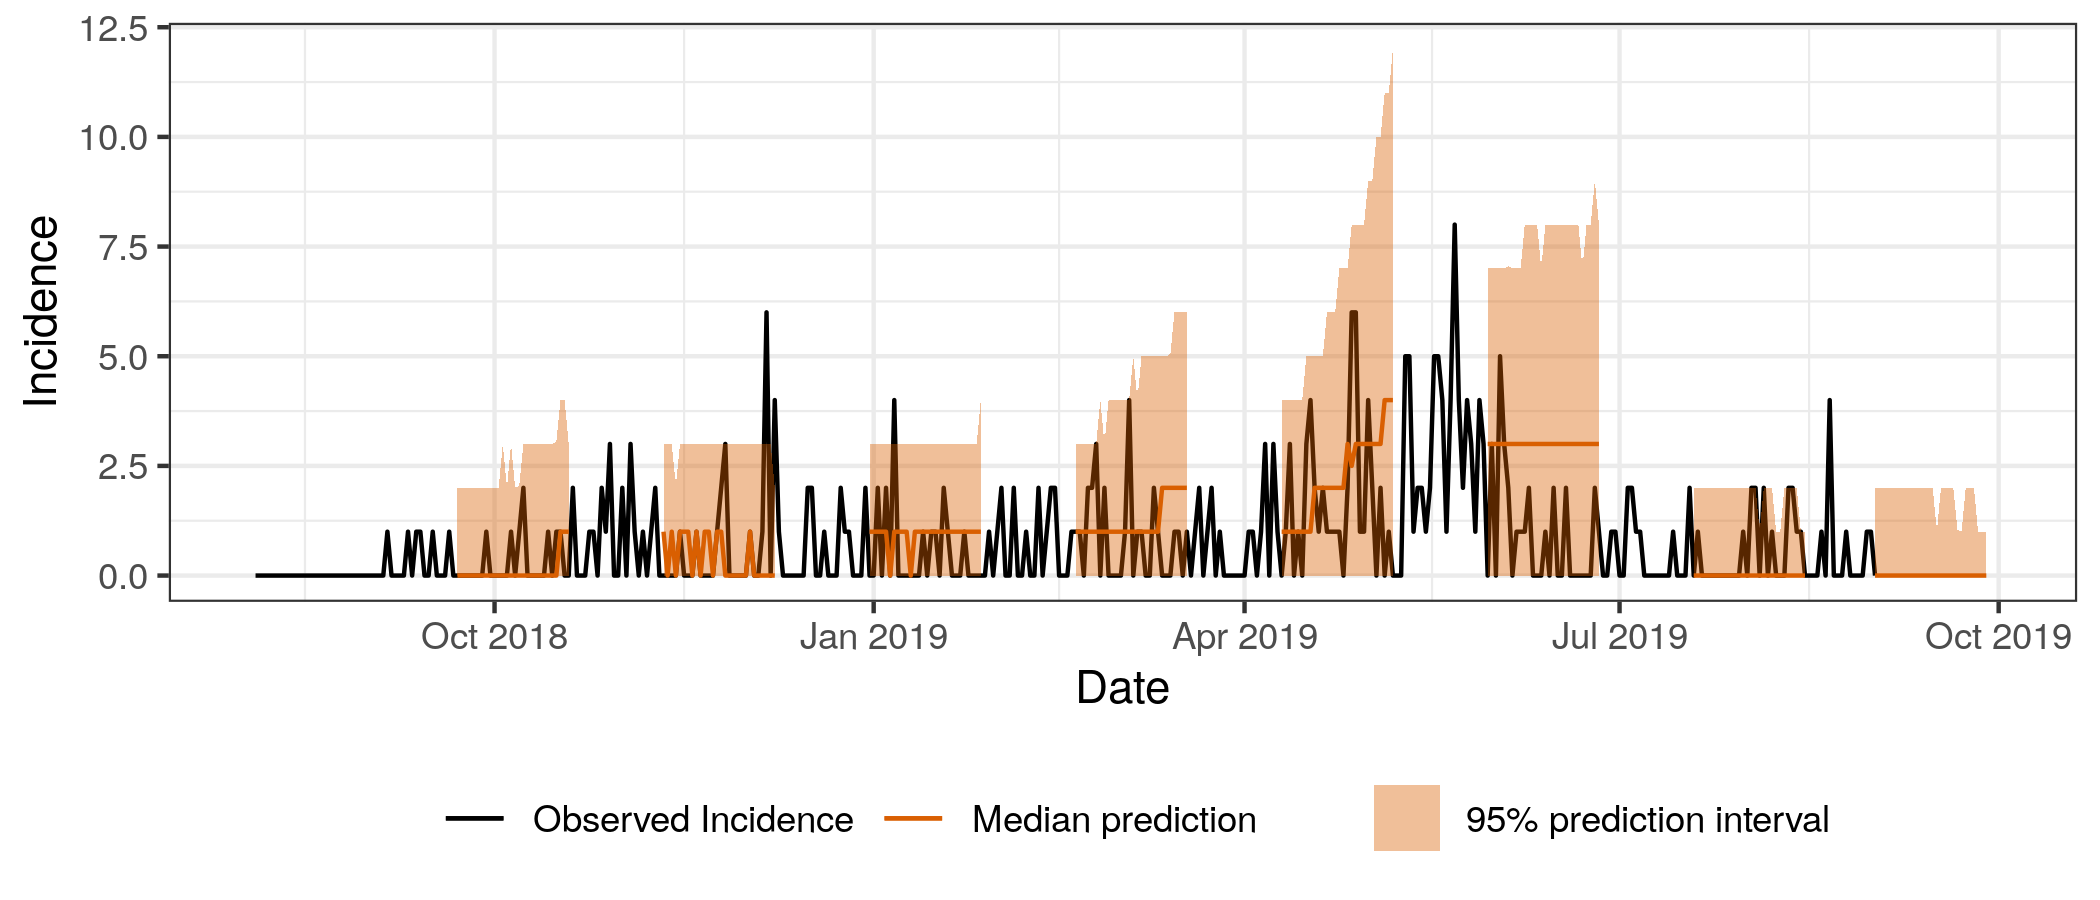
\includegraphics[width=0.9\linewidth, height=7cm]{../output/Butembo_predictions.png}  \caption{Forecasted and predicted incidence for the semilocal poisson model}\end{subfigure}

\begin{subfigure}{\textwidth}  \centering  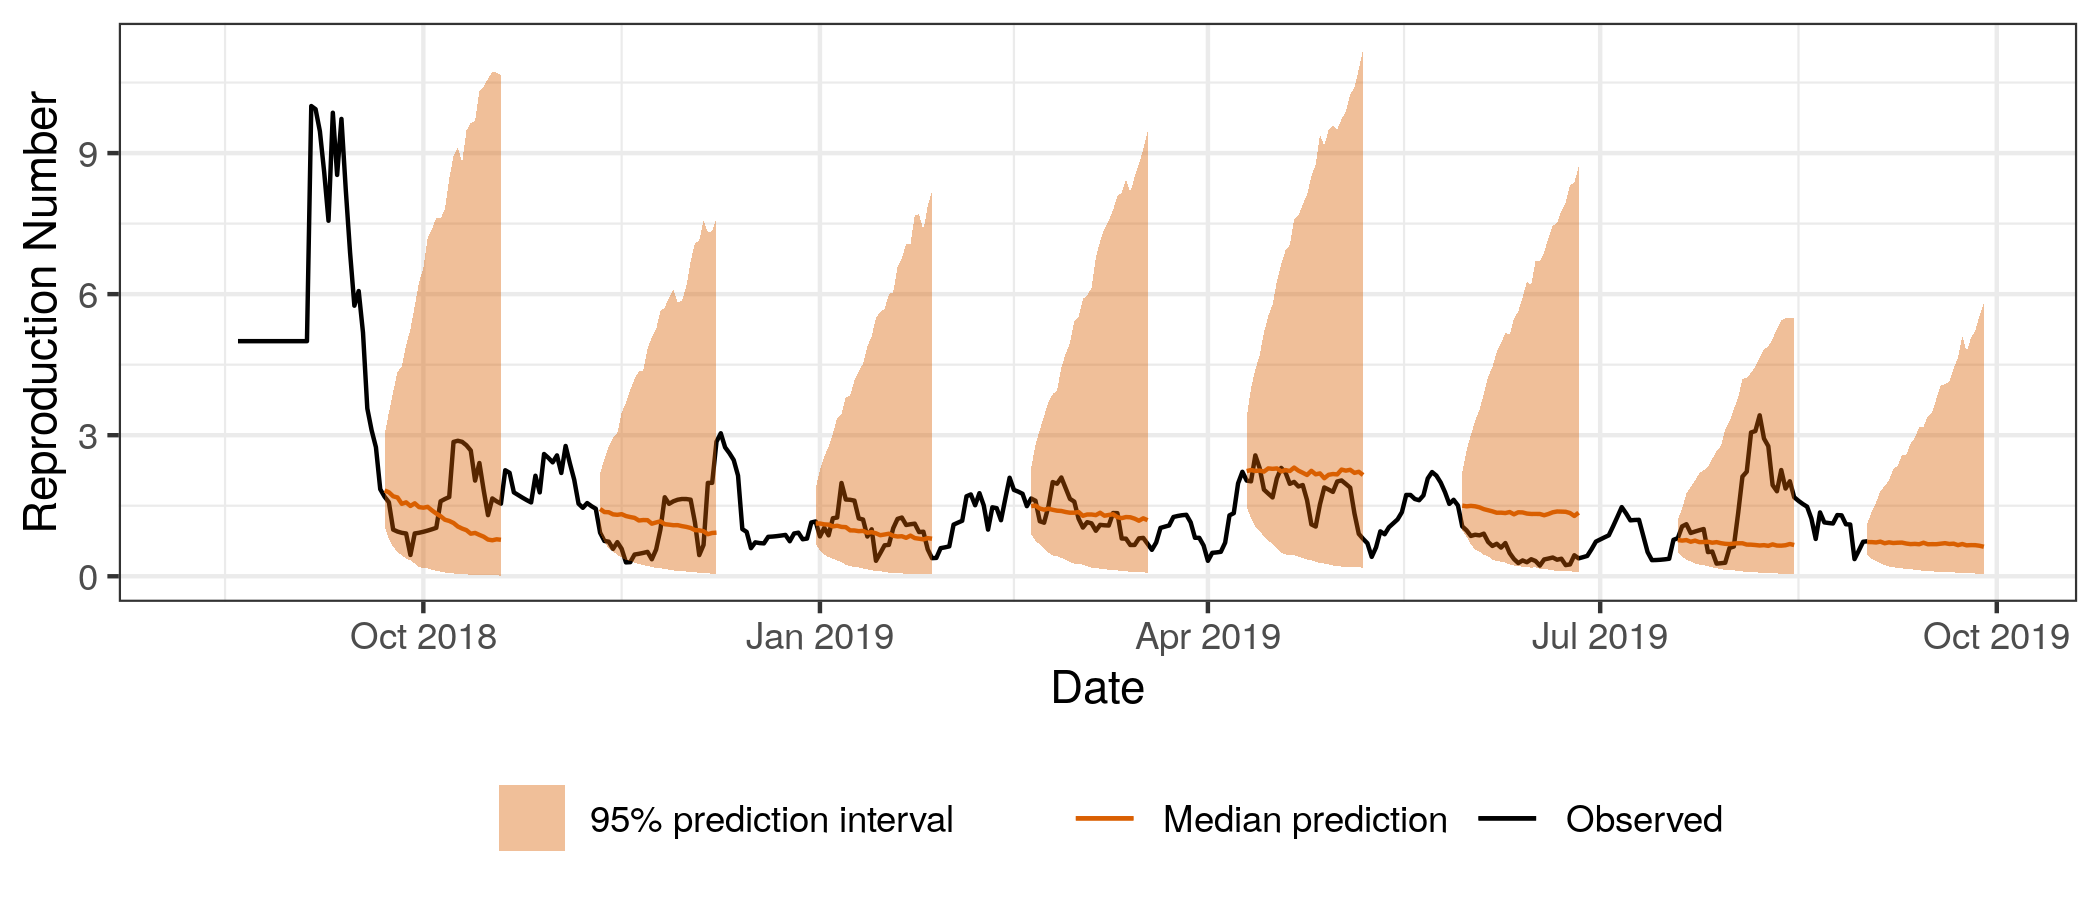
\includegraphics[width=0.9\linewidth, height=7cm]{../output/Butembo_Rs.png}  \caption{Forecasted and predicted repreoduction numbers for the semilocal poisson model}\end{subfigure}  \caption{Median forecast with 95 \% prediction intervals and observed values for incidence and reproduction number for the semilocal poisson model for Butembo.}\end{figure}

\begin{figure}[H]
\begin{subfigure}{0.5\textwidth}
  \centering
  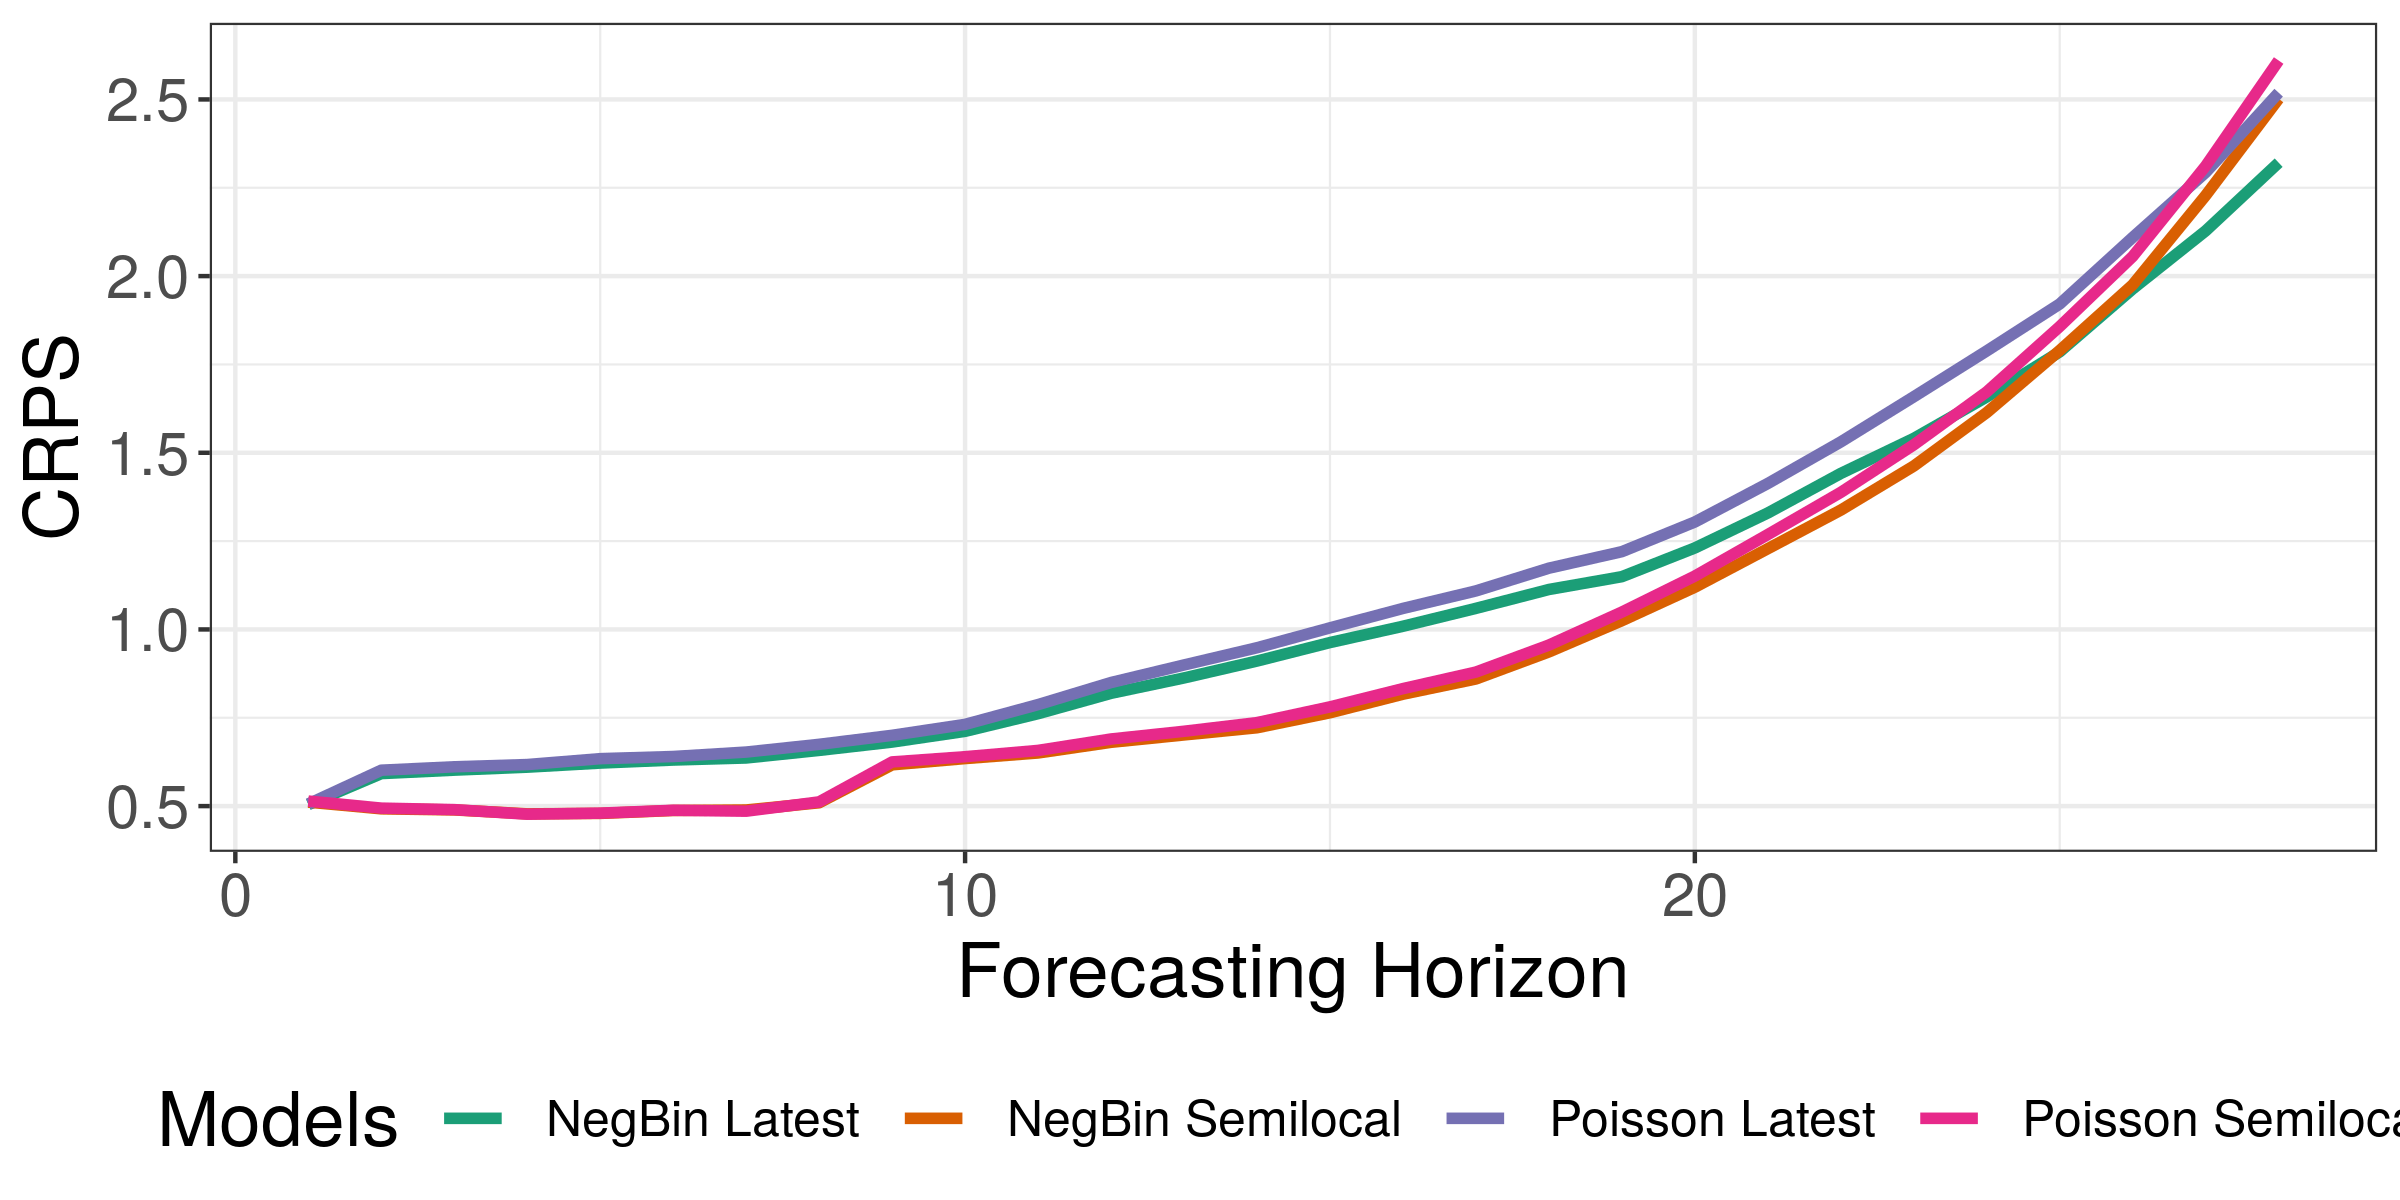
\includegraphics[width=\linewidth]{../output/Butembo_crps.png}  
  \caption{Contineously Ranked Probability Score}
  \label{fig:sub-first}
\end{subfigure}
\begin{subfigure}{0.5\textwidth}
  \centering
  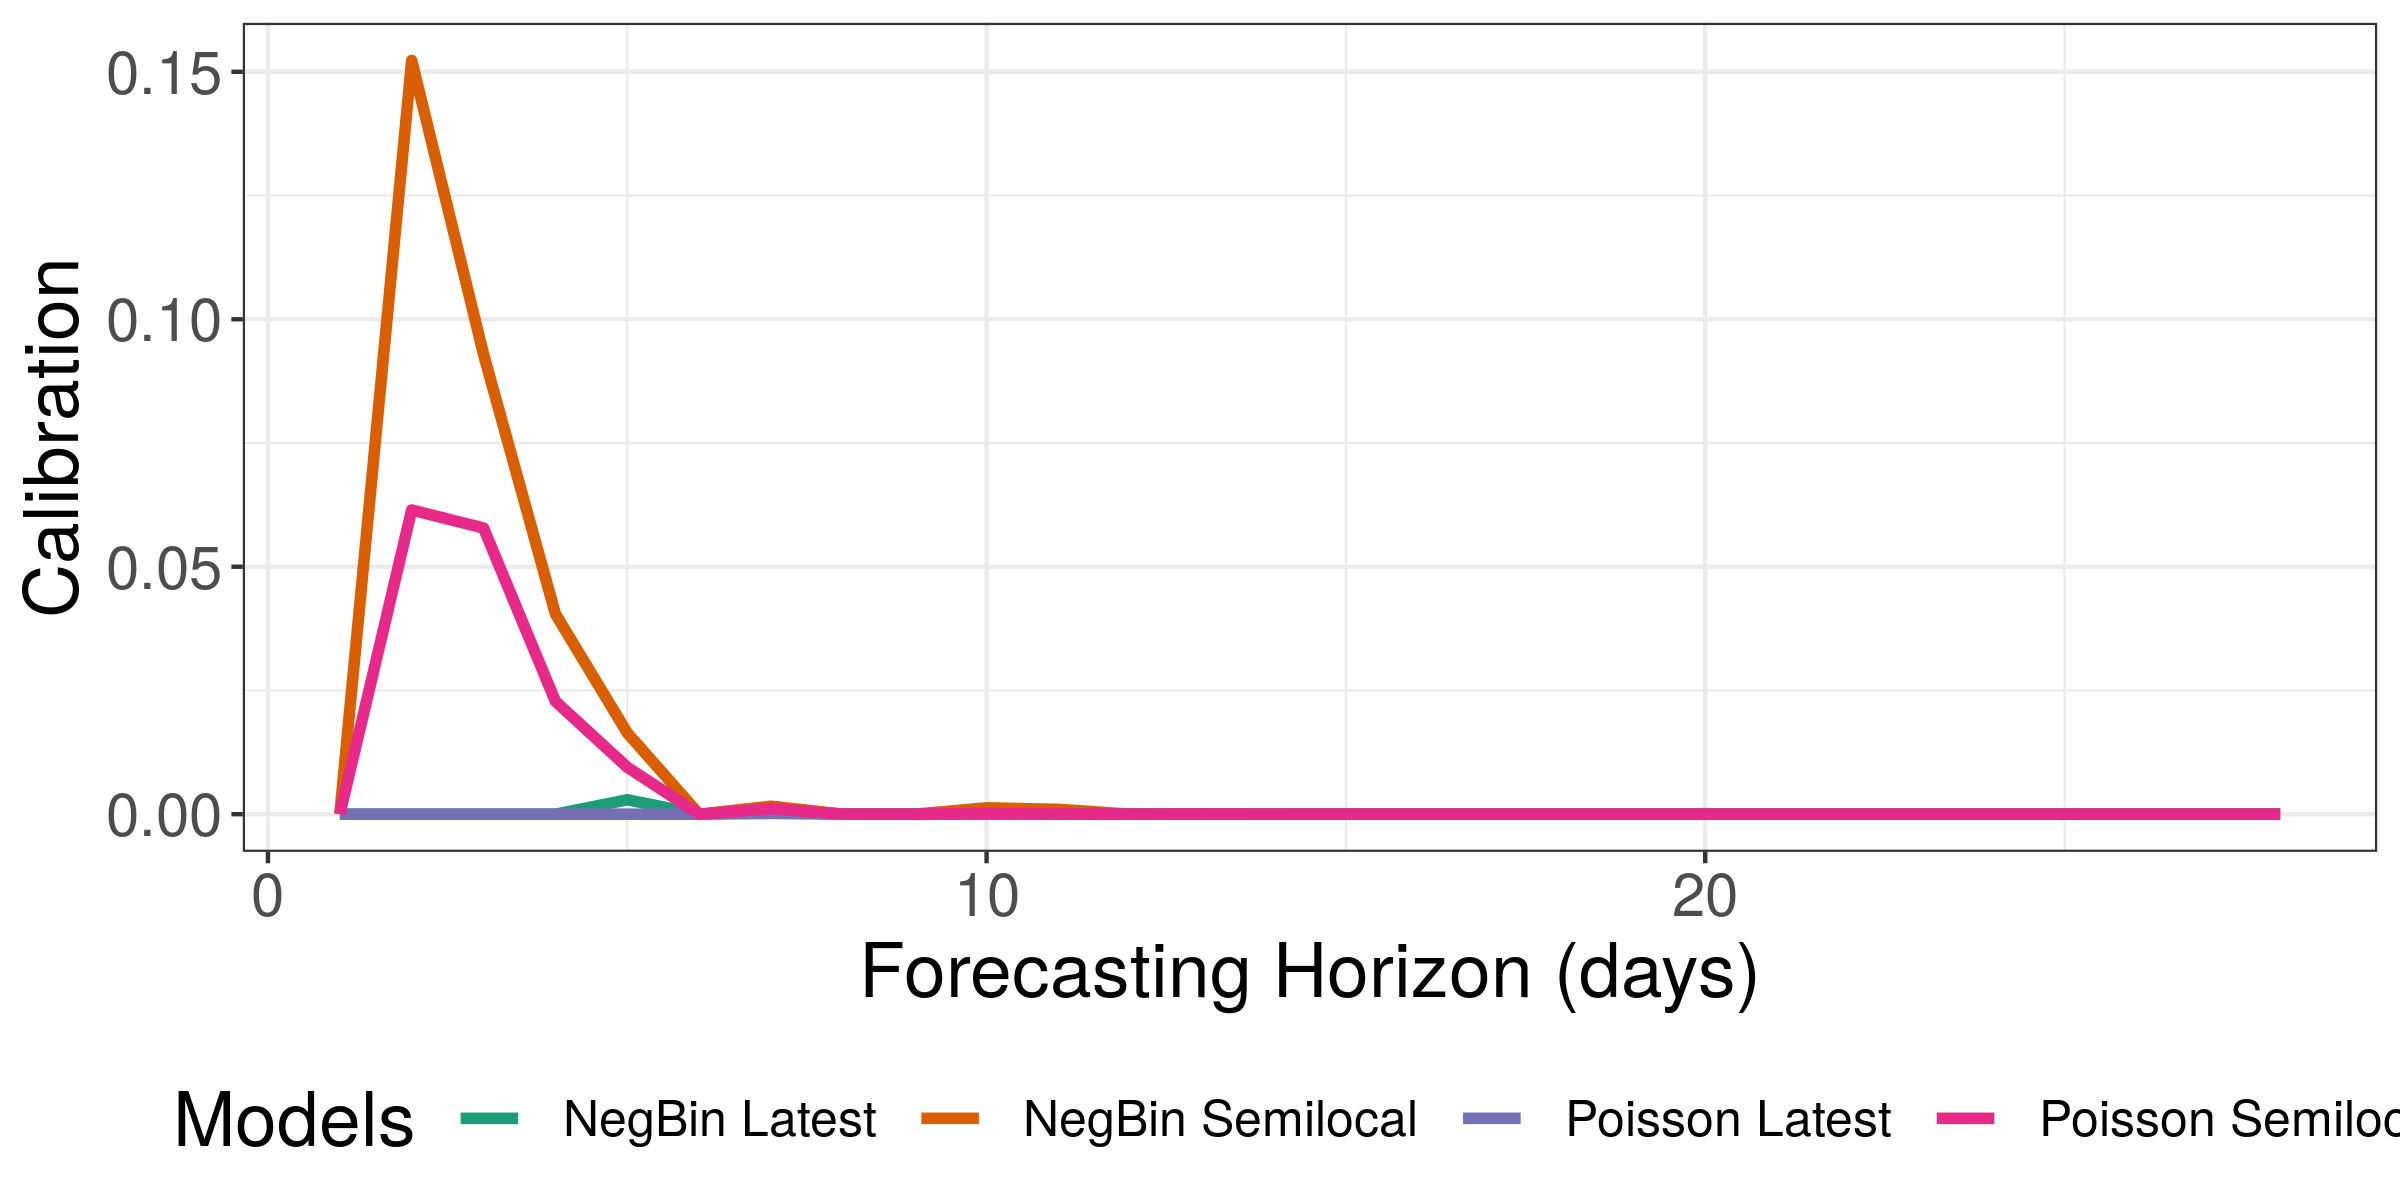
\includegraphics[width=\linewidth]{../output/Butembo_calibration.png}  
  \caption{Calibration p-value}
  \label{fig:sub-second}
\end{subfigure}

\begin{subfigure}{0.5\textwidth}
  \centering
  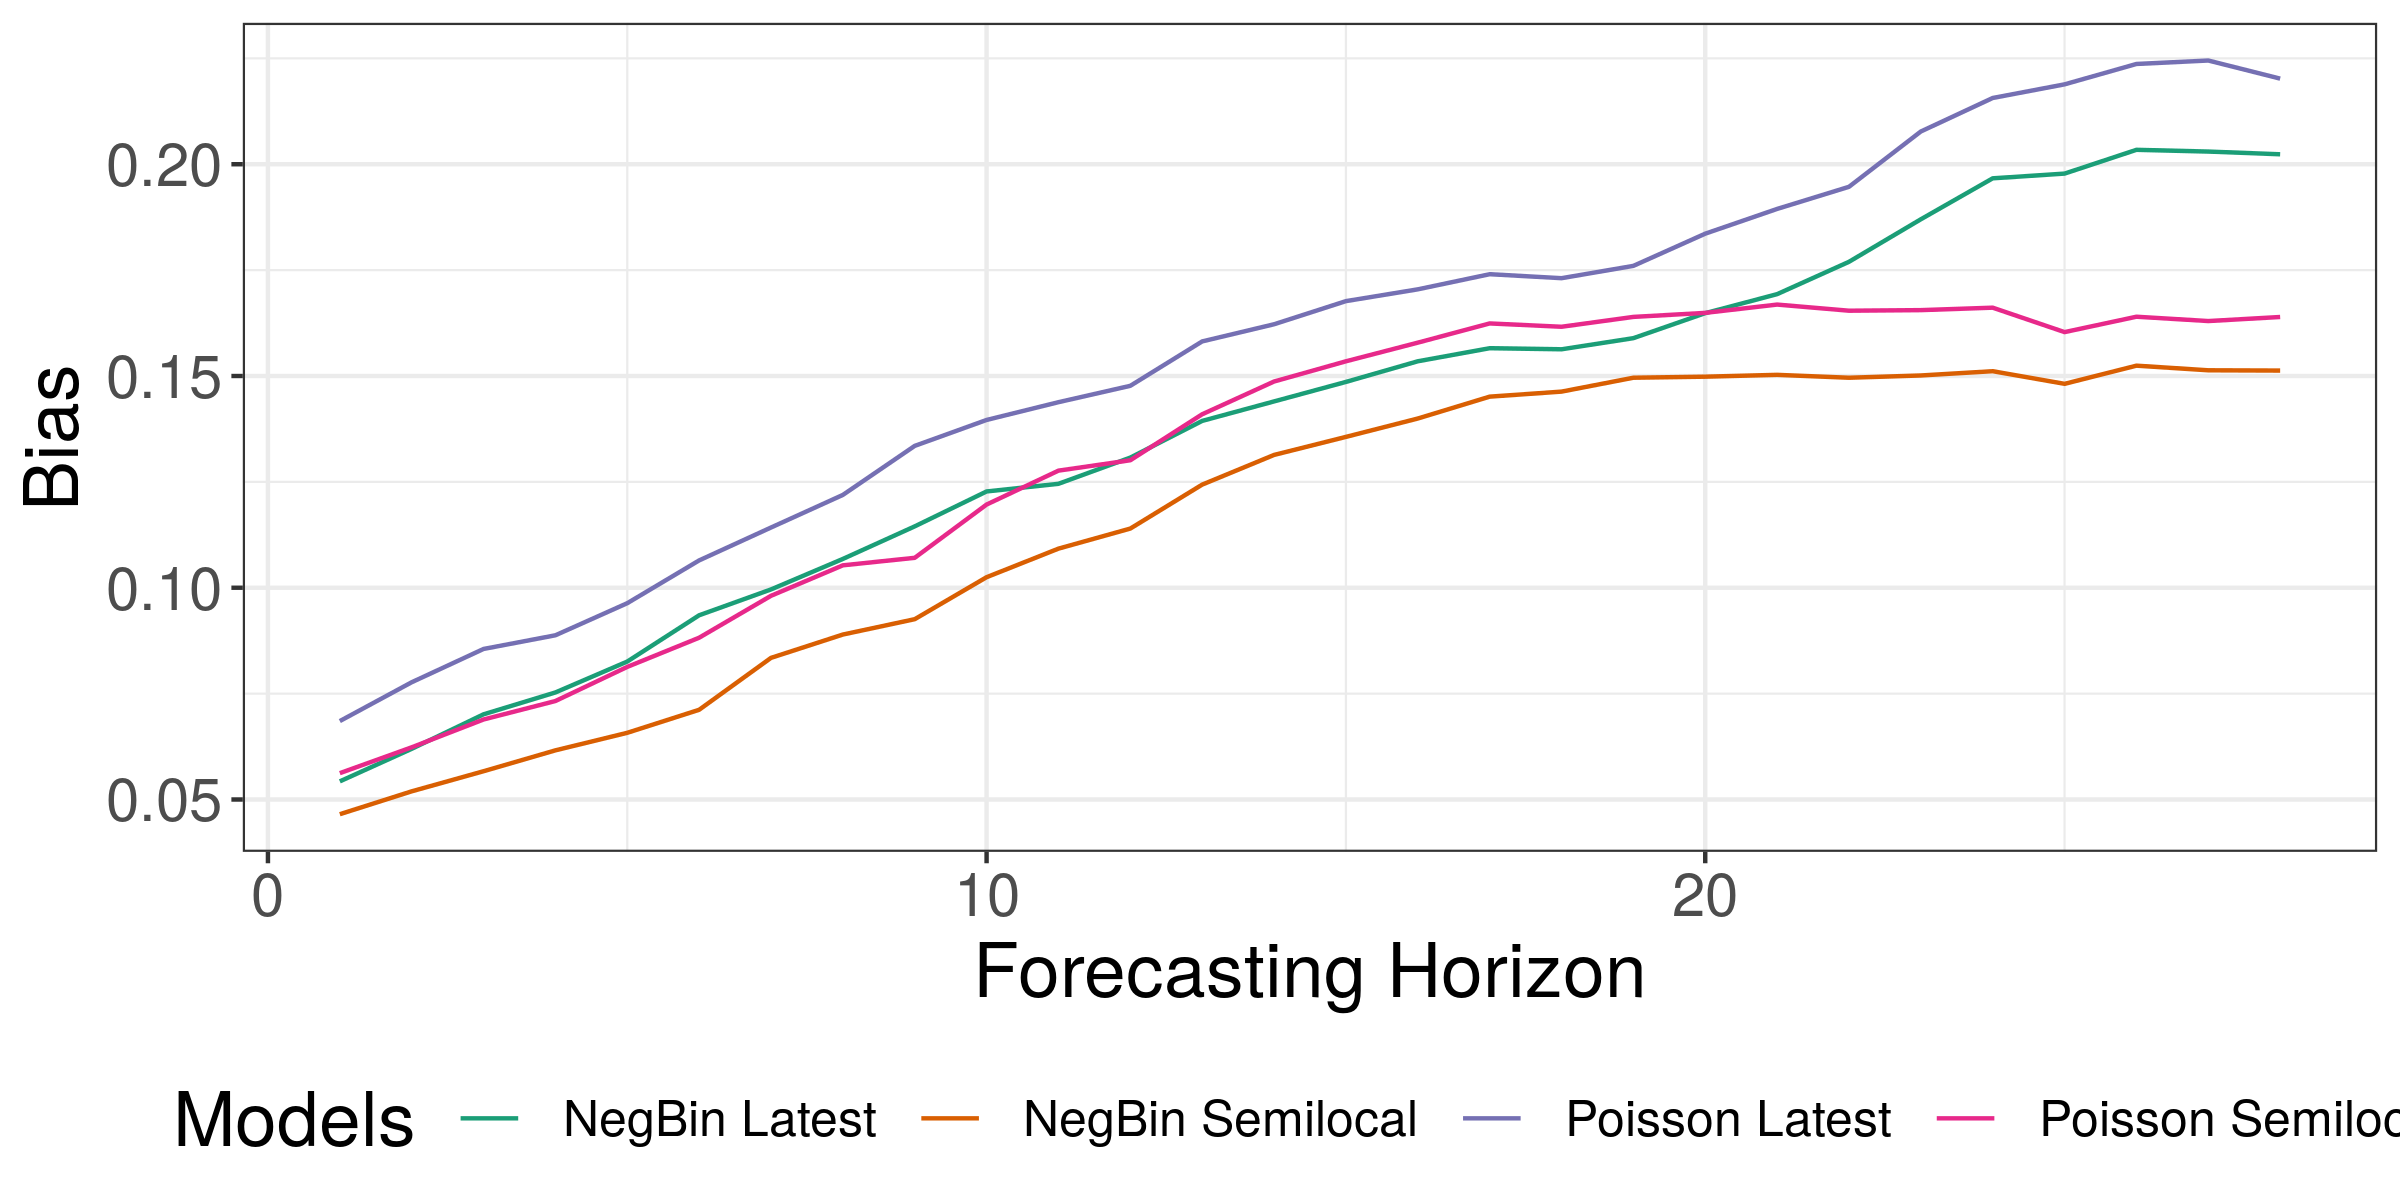
\includegraphics[width=\linewidth]{../output/Butembo_bias.png}  
  \caption{Bias}
  \label{fig:sub-third}
\end{subfigure}
\begin{subfigure}{0.5\textwidth}
  \centering
  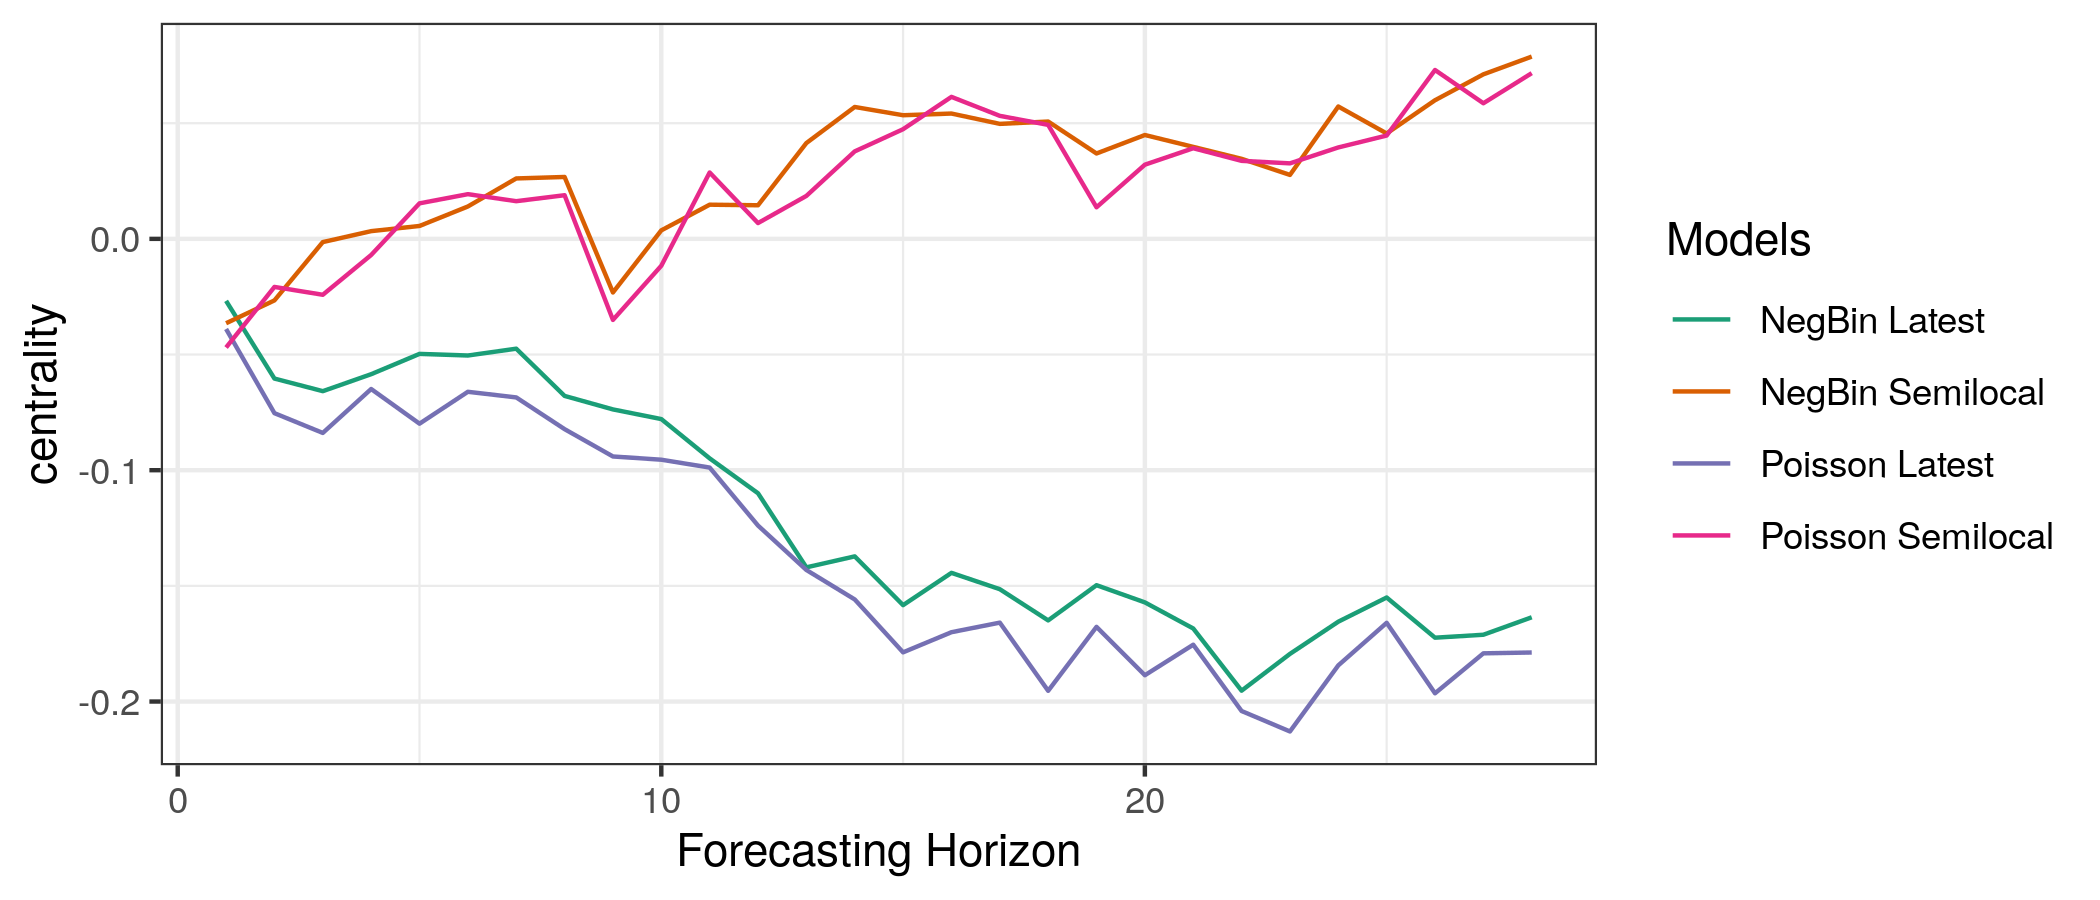
\includegraphics[width=\linewidth]{../output/Butembo_centrality.png}  
  \caption{Centrality of PIT values}
  \label{fig:nat_scores_4}
\end{subfigure}
  \caption{Scores for the entire outbreak as a function of the forecasting horizon.}

  \label{fig:nat_scores}
\end{figure}
 \section{ Kalunguta }\begin{figure}[H]\begin{subfigure}{\textwidth}  \centering  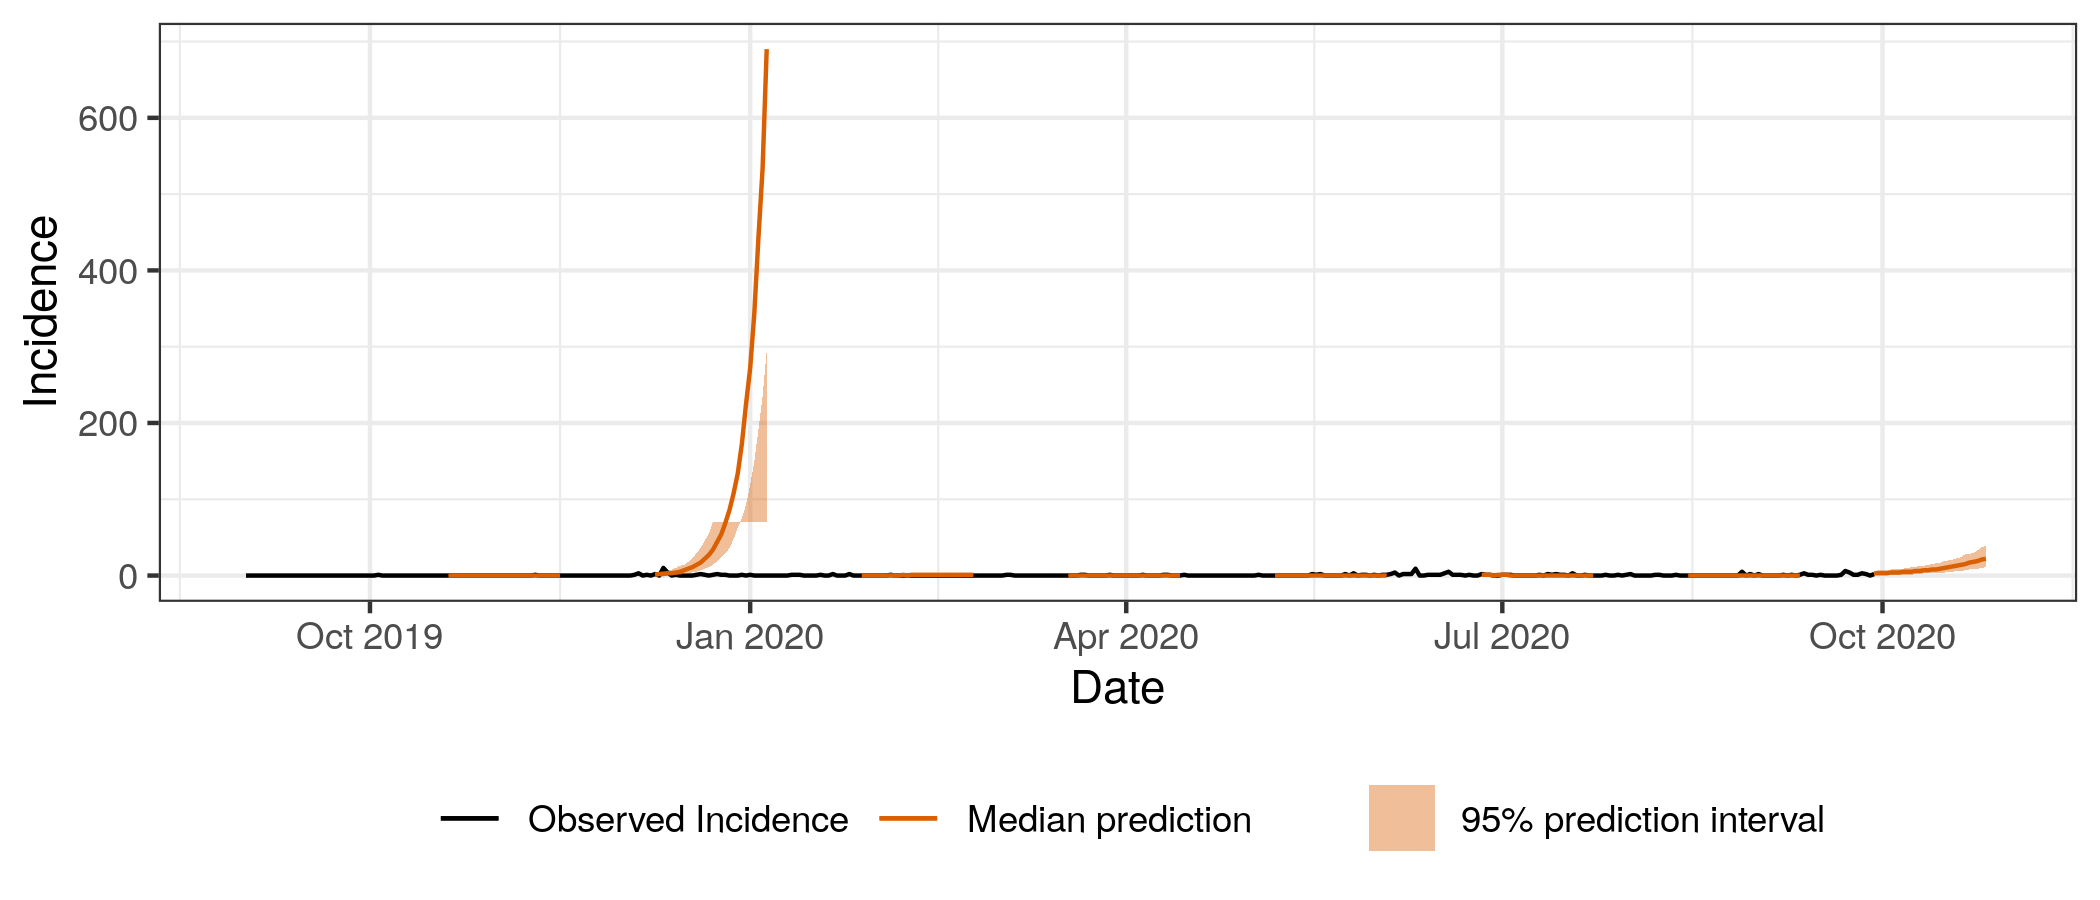
\includegraphics[width=0.9\linewidth, height=7cm]{../output/Kalunguta_predictions.png}  \caption{Forecasted and predicted incidence for the semilocal poisson model}\end{subfigure}

\begin{subfigure}{\textwidth}  \centering  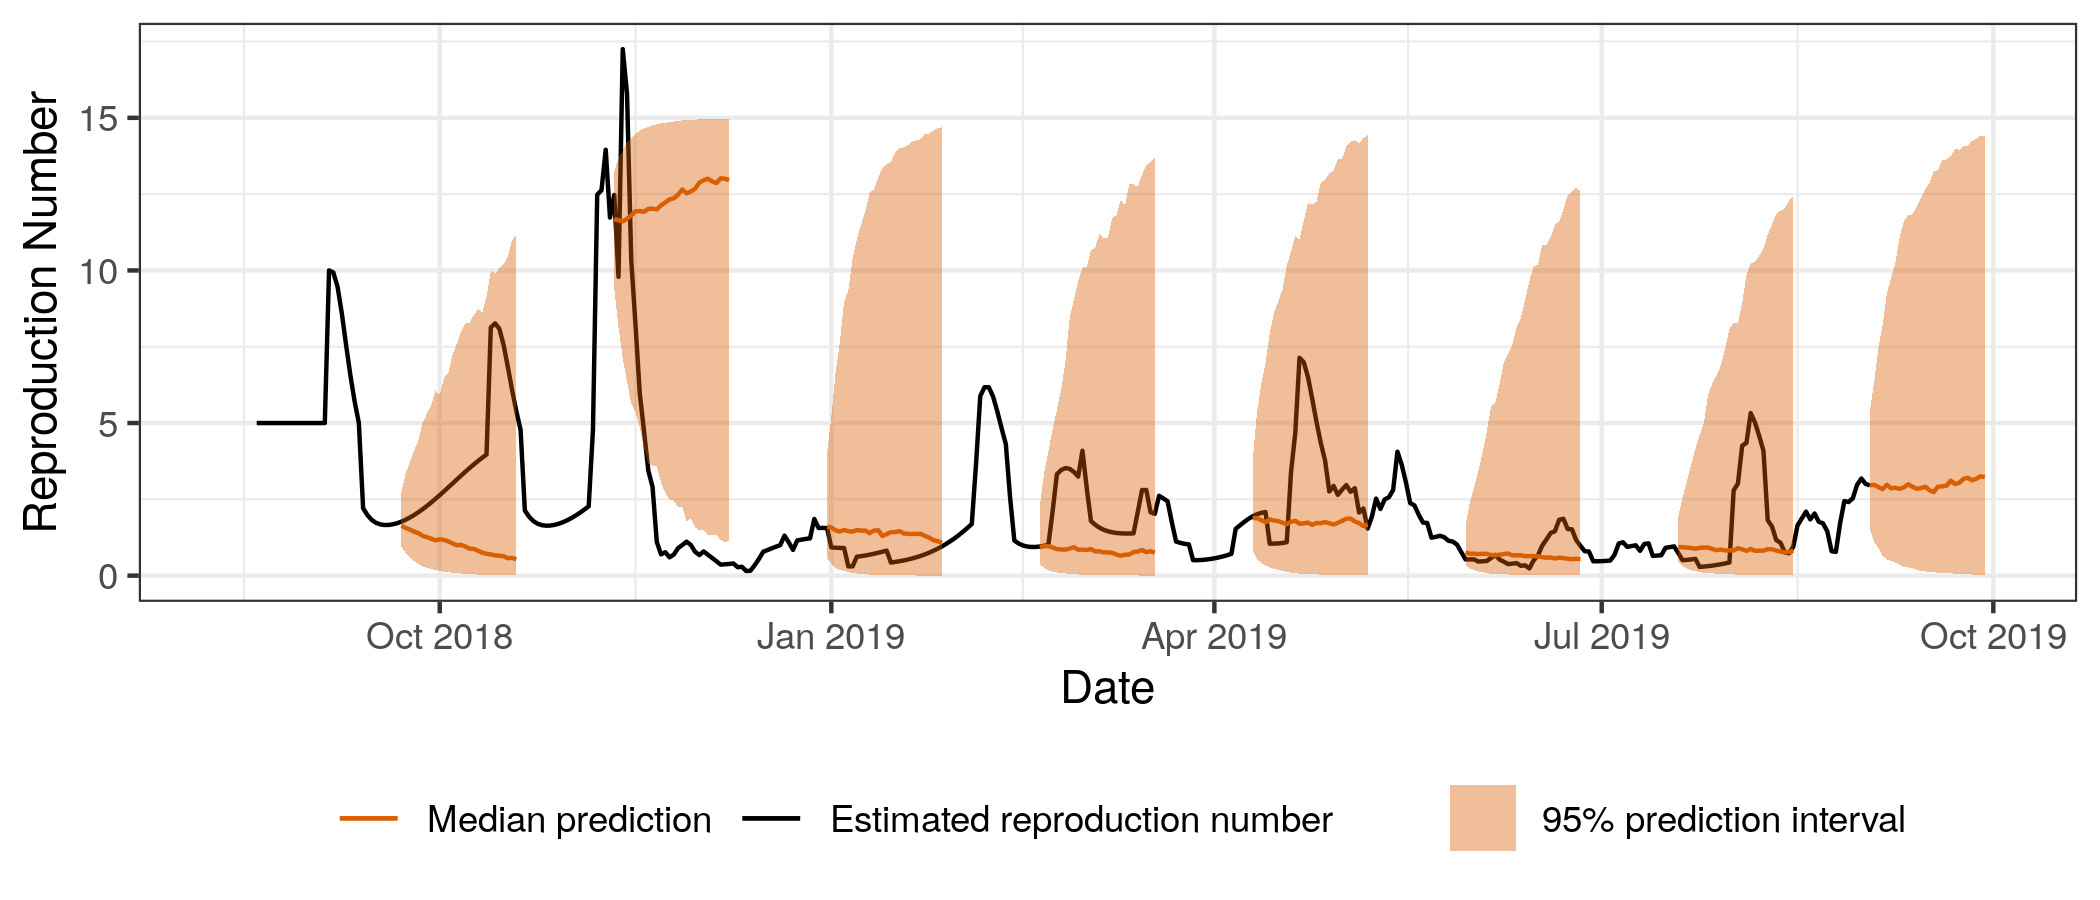
\includegraphics[width=0.9\linewidth, height=7cm]{../output/Kalunguta_Rs.png}  \caption{Forecasted and predicted repreoduction numbers for the semilocal poisson model}\end{subfigure}  \caption{Median forecast with 95 \% prediction intervals and observed values for incidence and reproduction number for the semilocal poisson model for Kalunguta.}\end{figure}

\begin{figure}[H]
\begin{subfigure}{0.5\textwidth}
  \centering
  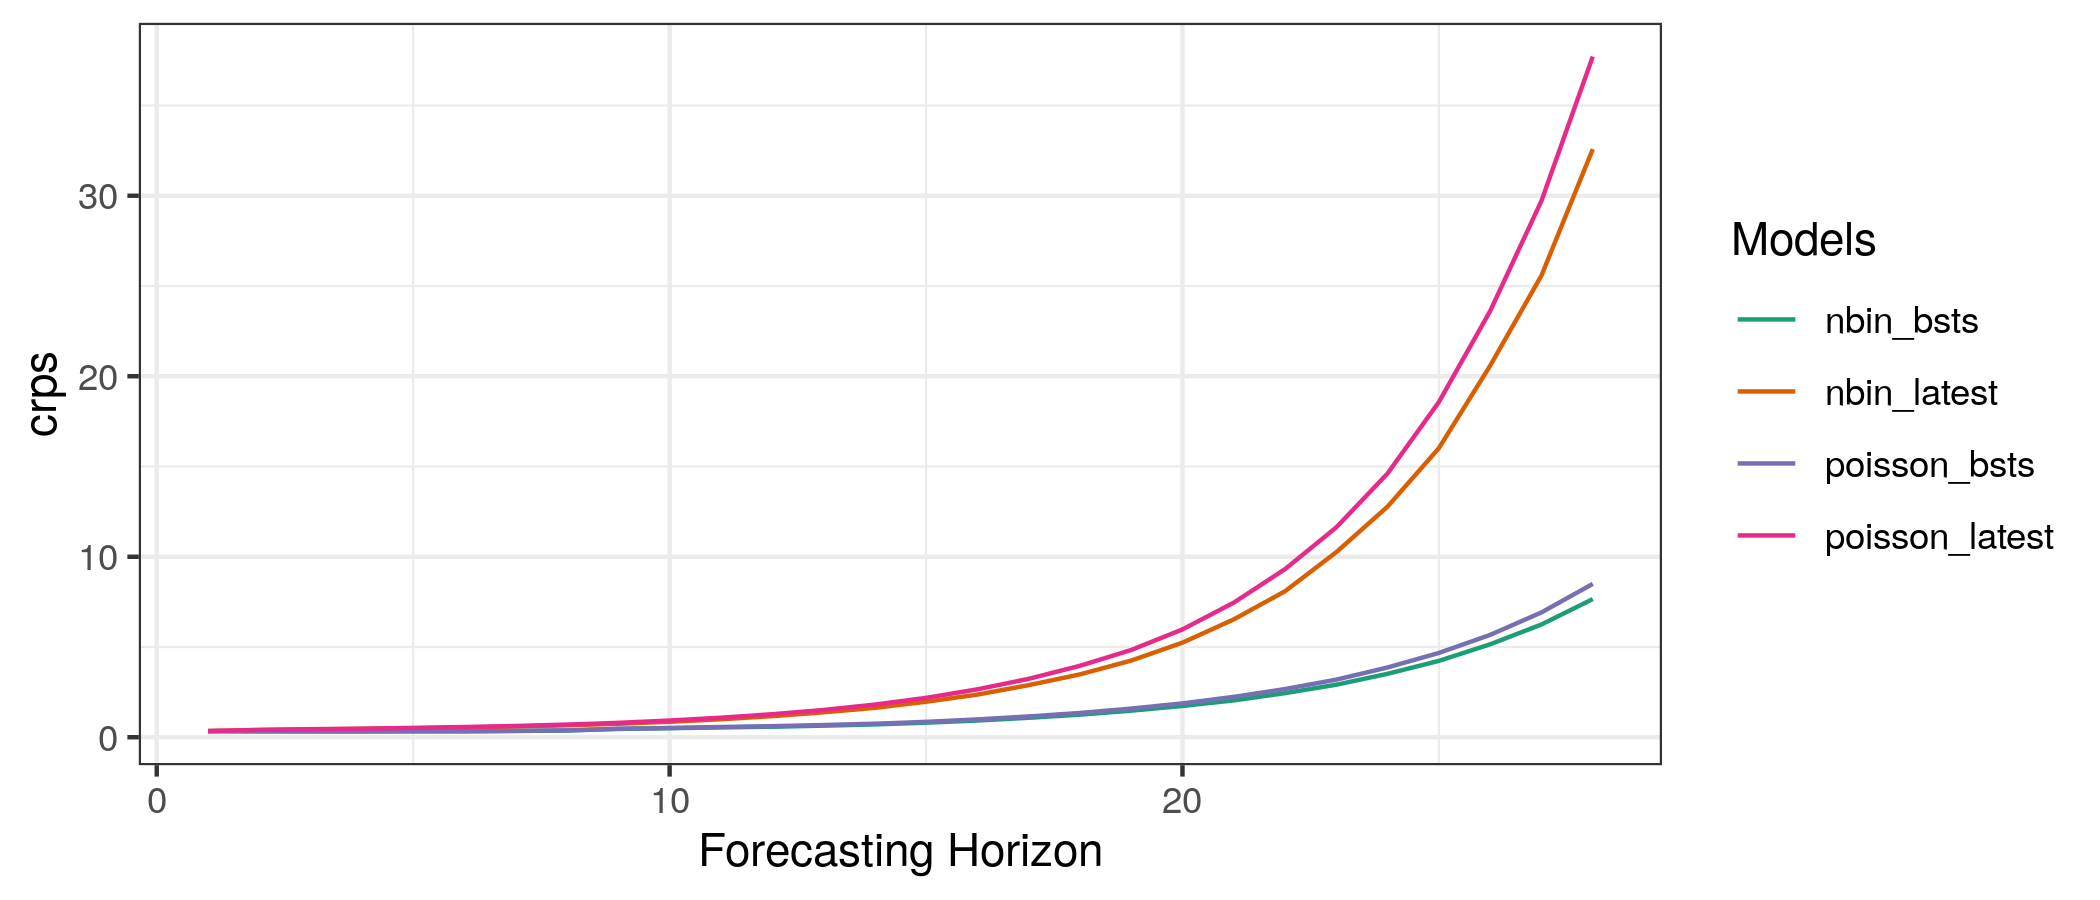
\includegraphics[width=\linewidth]{../output/Kalunguta_crps.png}  
  \caption{Contineously Ranked Probability Score}
  \label{fig:sub-first}
\end{subfigure}
\begin{subfigure}{0.5\textwidth}
  \centering
  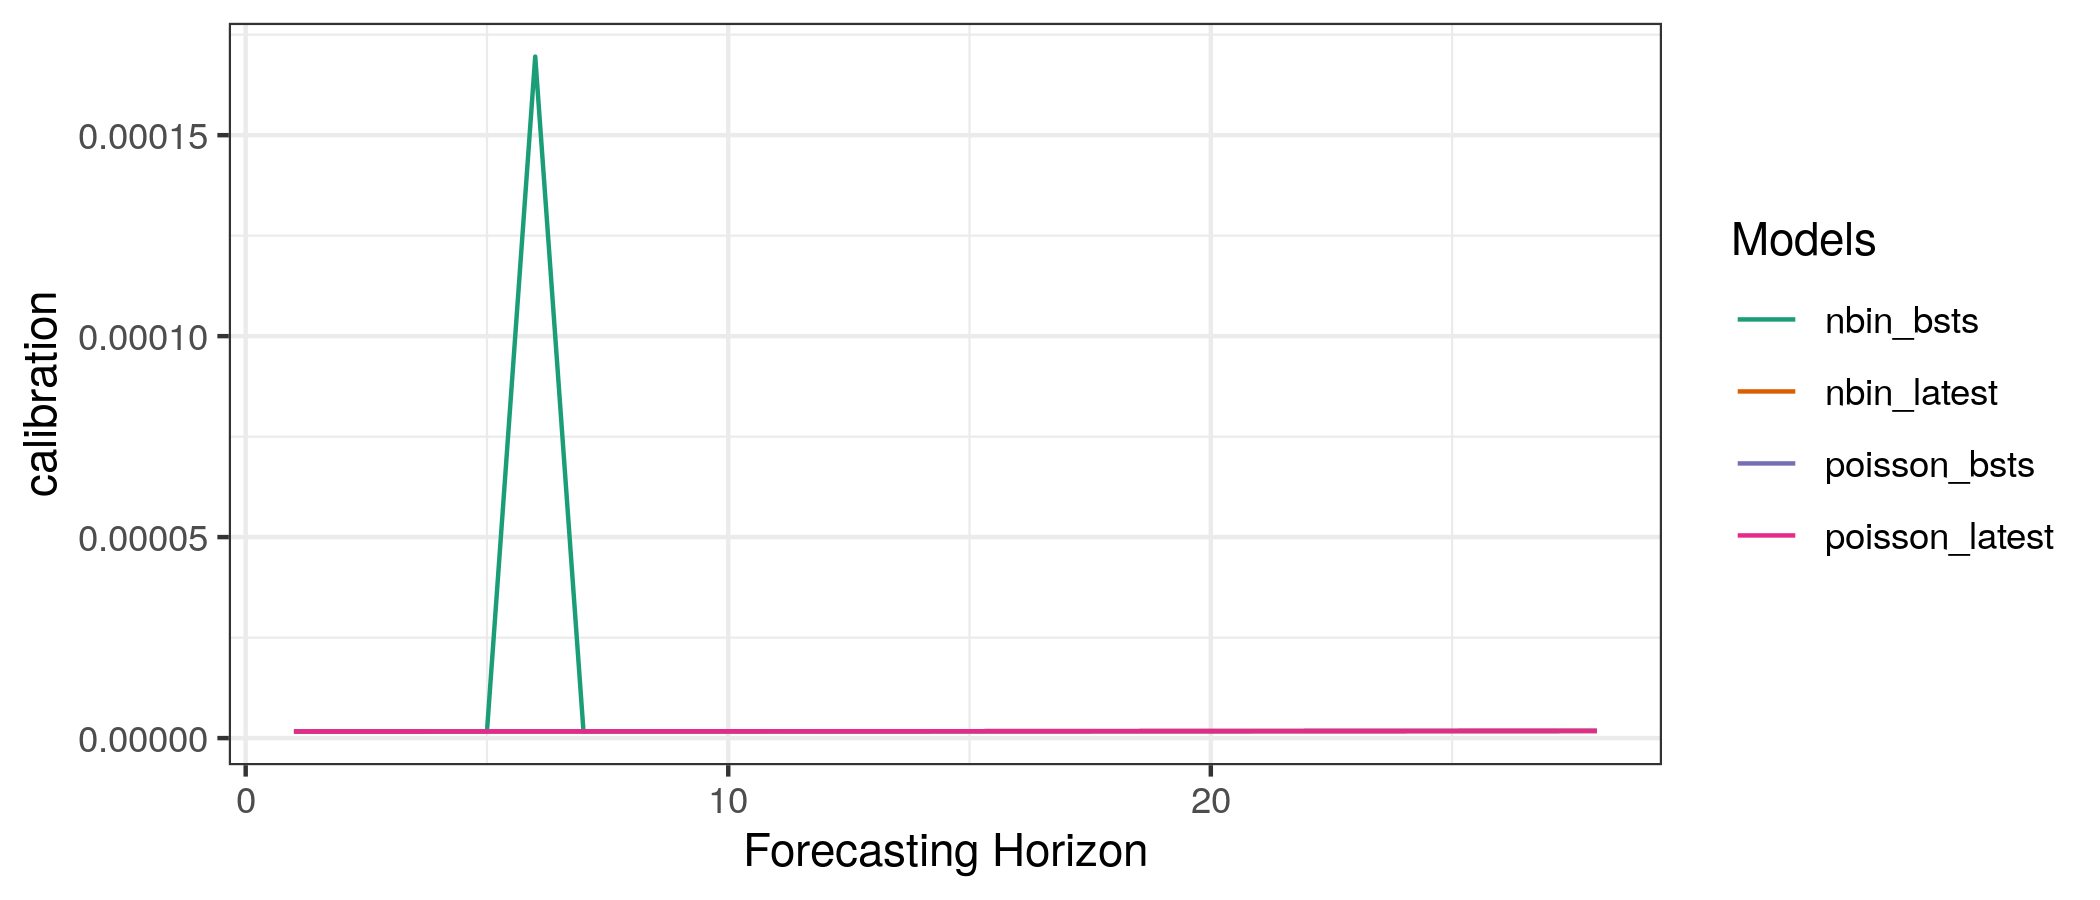
\includegraphics[width=\linewidth]{../output/Kalunguta_calibration.png}  
  \caption{Calibration p-value}
  \label{fig:sub-second}
\end{subfigure}

\begin{subfigure}{0.5\textwidth}
  \centering
  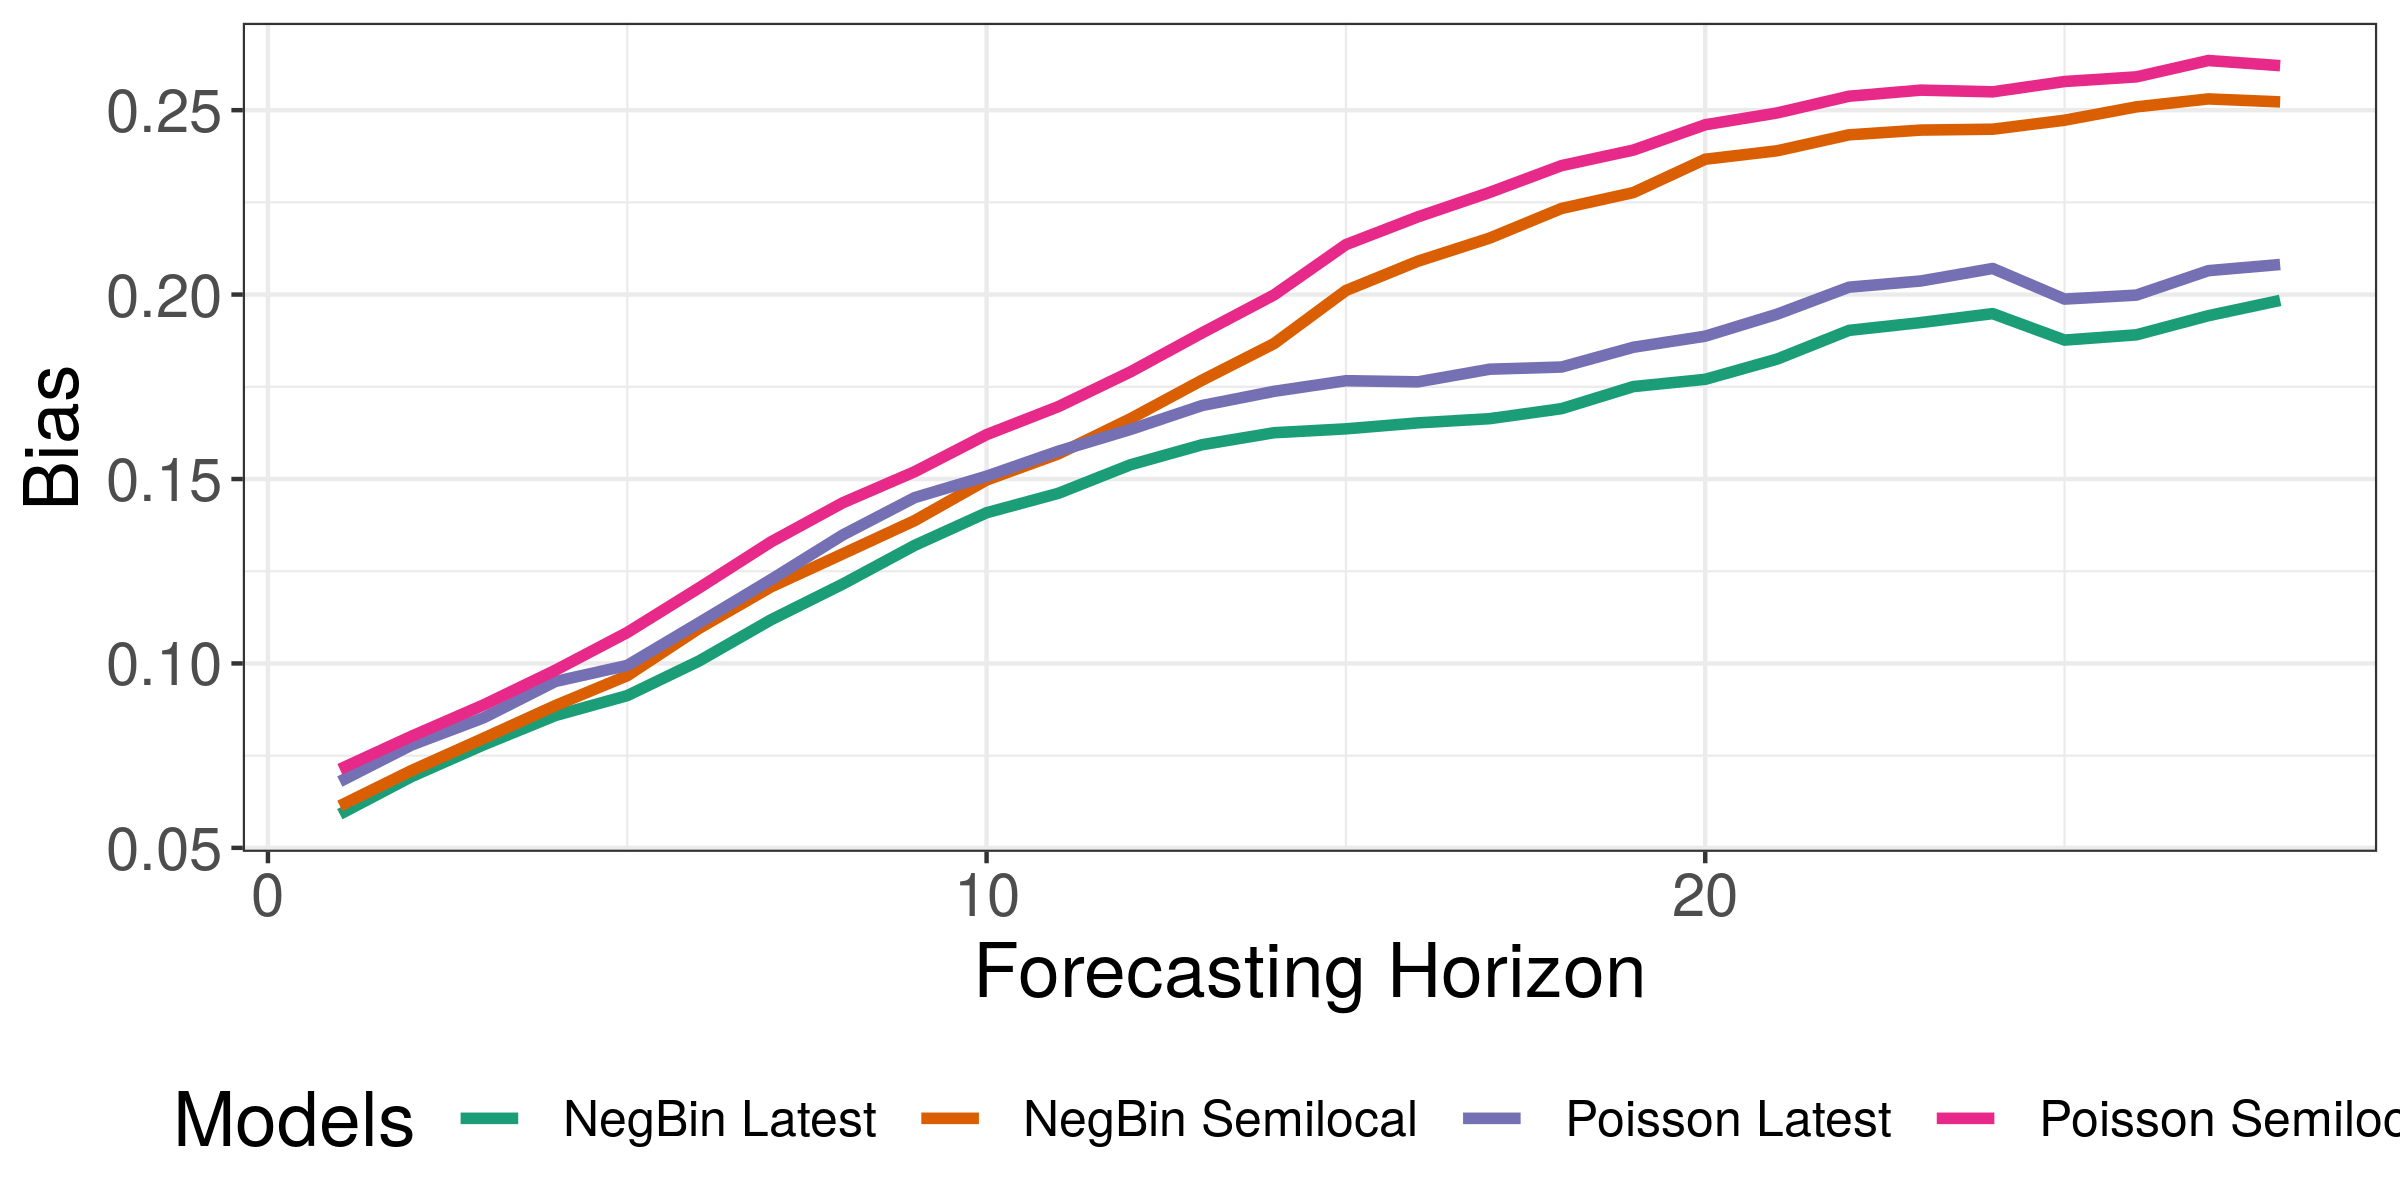
\includegraphics[width=\linewidth]{../output/Kalunguta_bias.png}  
  \caption{Bias}
  \label{fig:sub-third}
\end{subfigure}
\begin{subfigure}{0.5\textwidth}
  \centering
  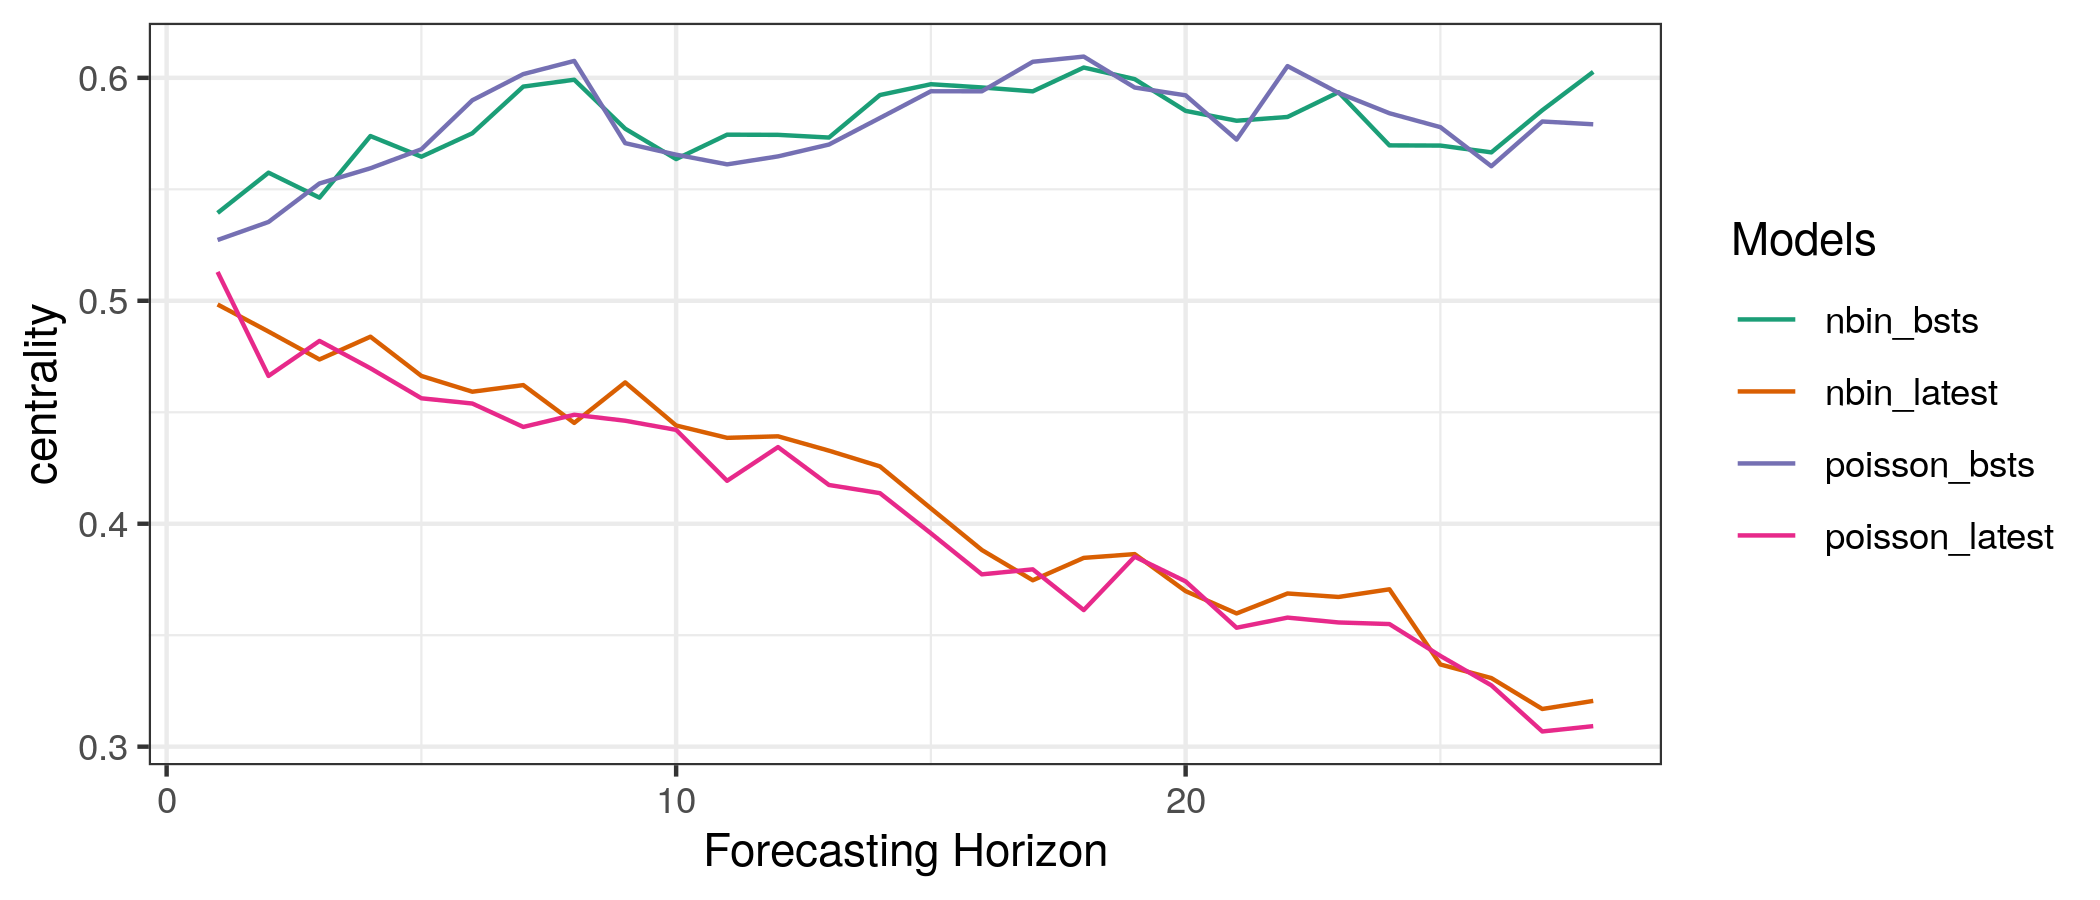
\includegraphics[width=\linewidth]{../output/Kalunguta_centrality.png}  
  \caption{Centrality of PIT values}
  \label{fig:nat_scores_4}
\end{subfigure}
  \caption{Scores for the entire outbreak as a function of the forecasting horizon.}

  \label{fig:nat_scores}
\end{figure}
 \section{ Katwa }\begin{figure}[H]\begin{subfigure}{\textwidth}  \centering  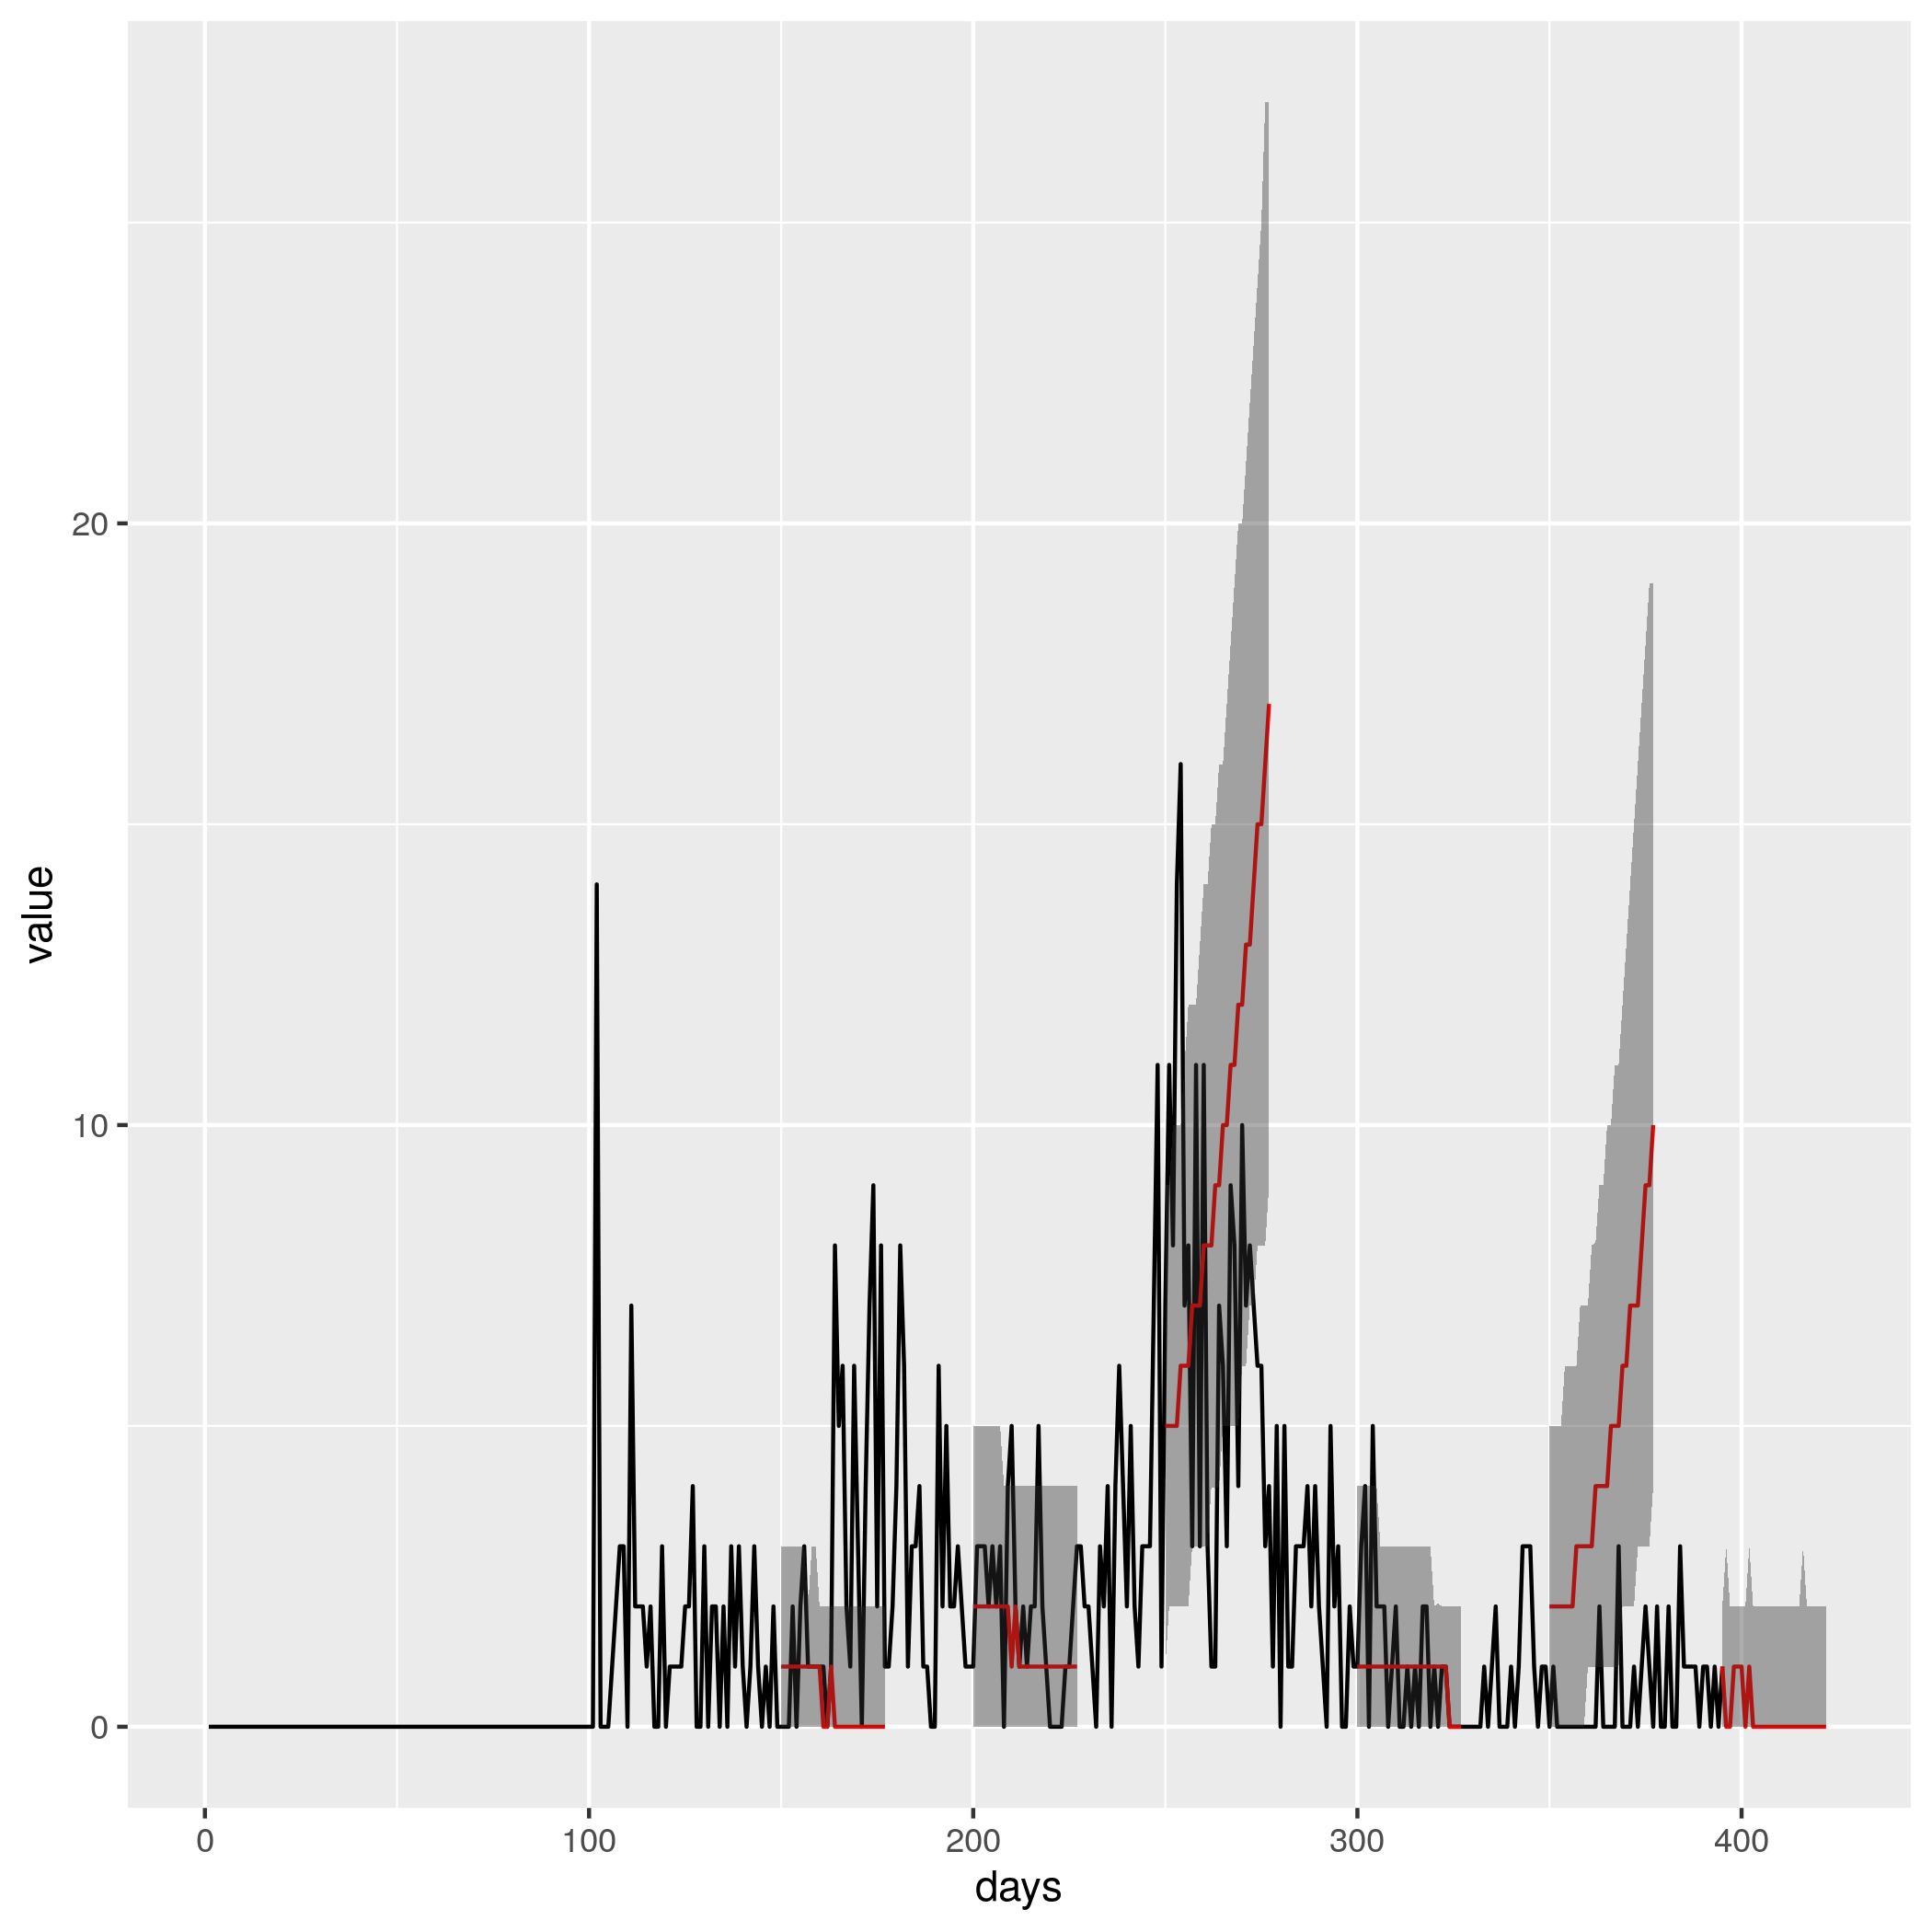
\includegraphics[width=0.9\linewidth, height=7cm]{../output/Katwa_predictions.png}  \caption{Forecasted and predicted incidence for the semilocal poisson model}\end{subfigure}

\begin{subfigure}{\textwidth}  \centering  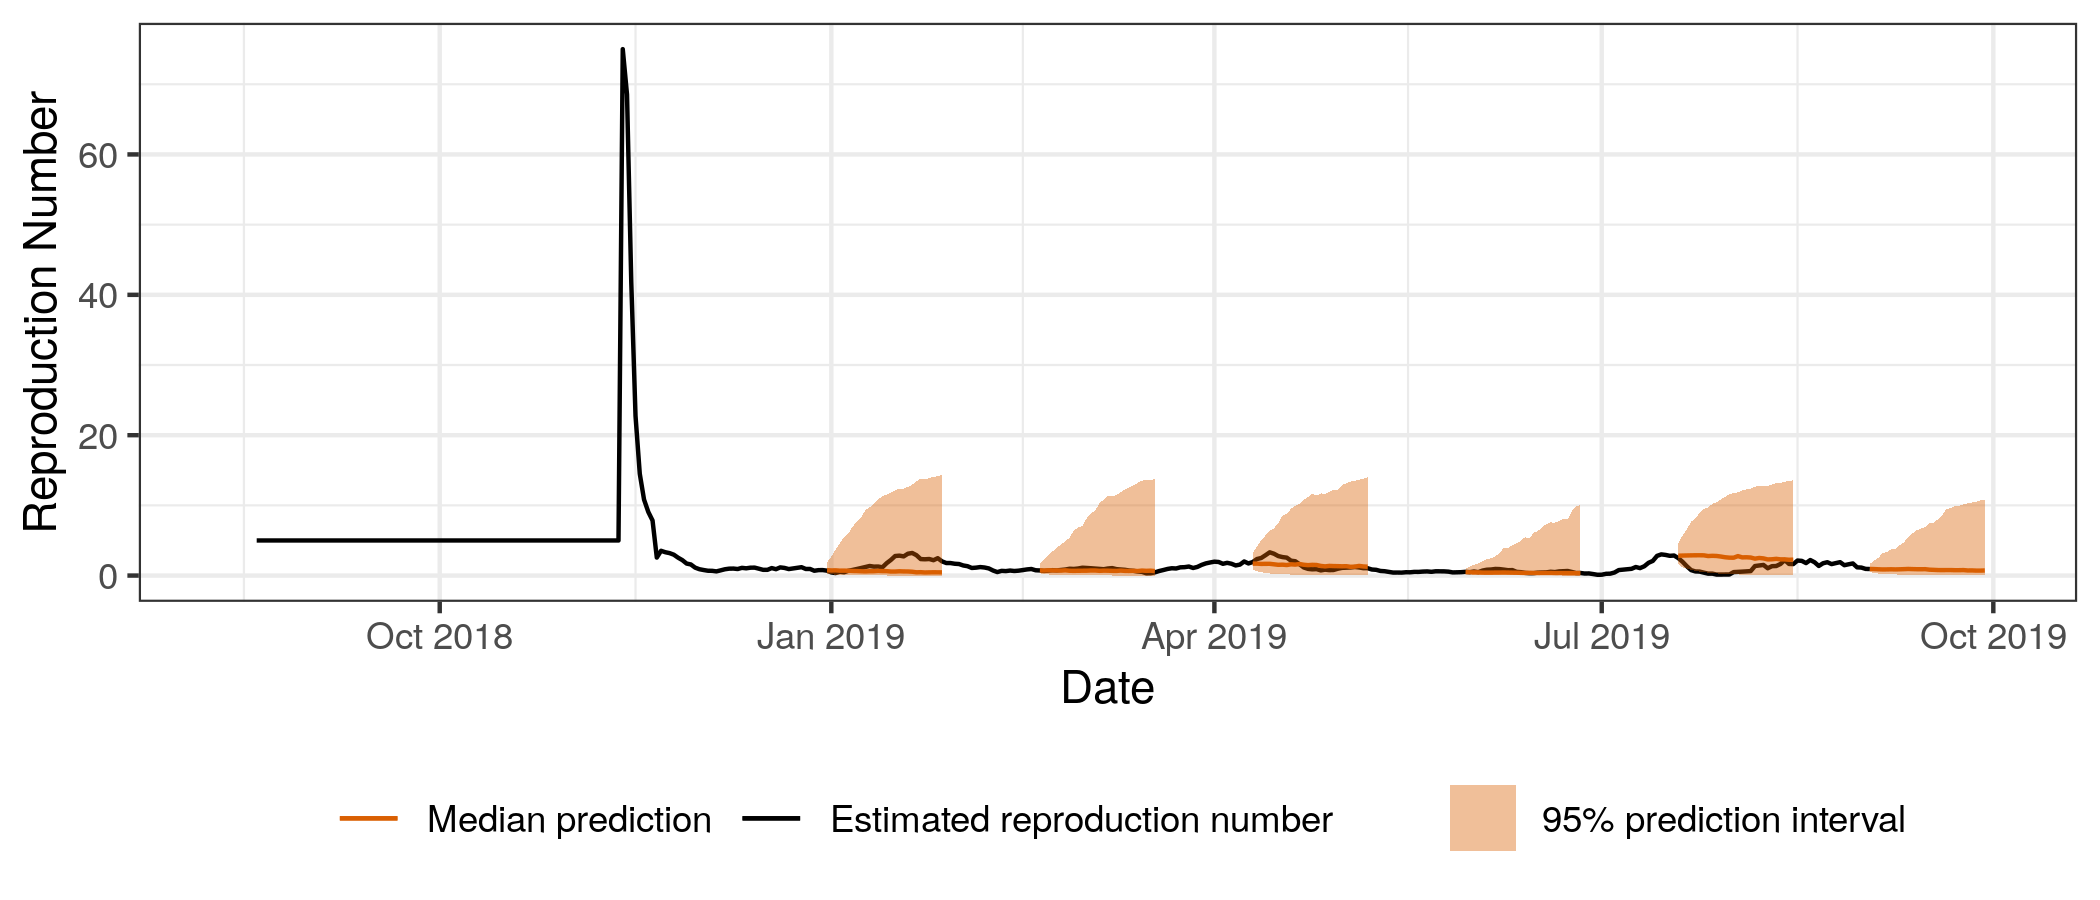
\includegraphics[width=0.9\linewidth, height=7cm]{../output/Katwa_Rs.png}  \caption{Forecasted and predicted repreoduction numbers for the semilocal poisson model}\end{subfigure}  \caption{Median forecast with 95 \% prediction intervals and observed values for incidence and reproduction number for the semilocal poisson model for Katwa.}\end{figure}

\begin{figure}[H]
\begin{subfigure}{0.5\textwidth}
  \centering
  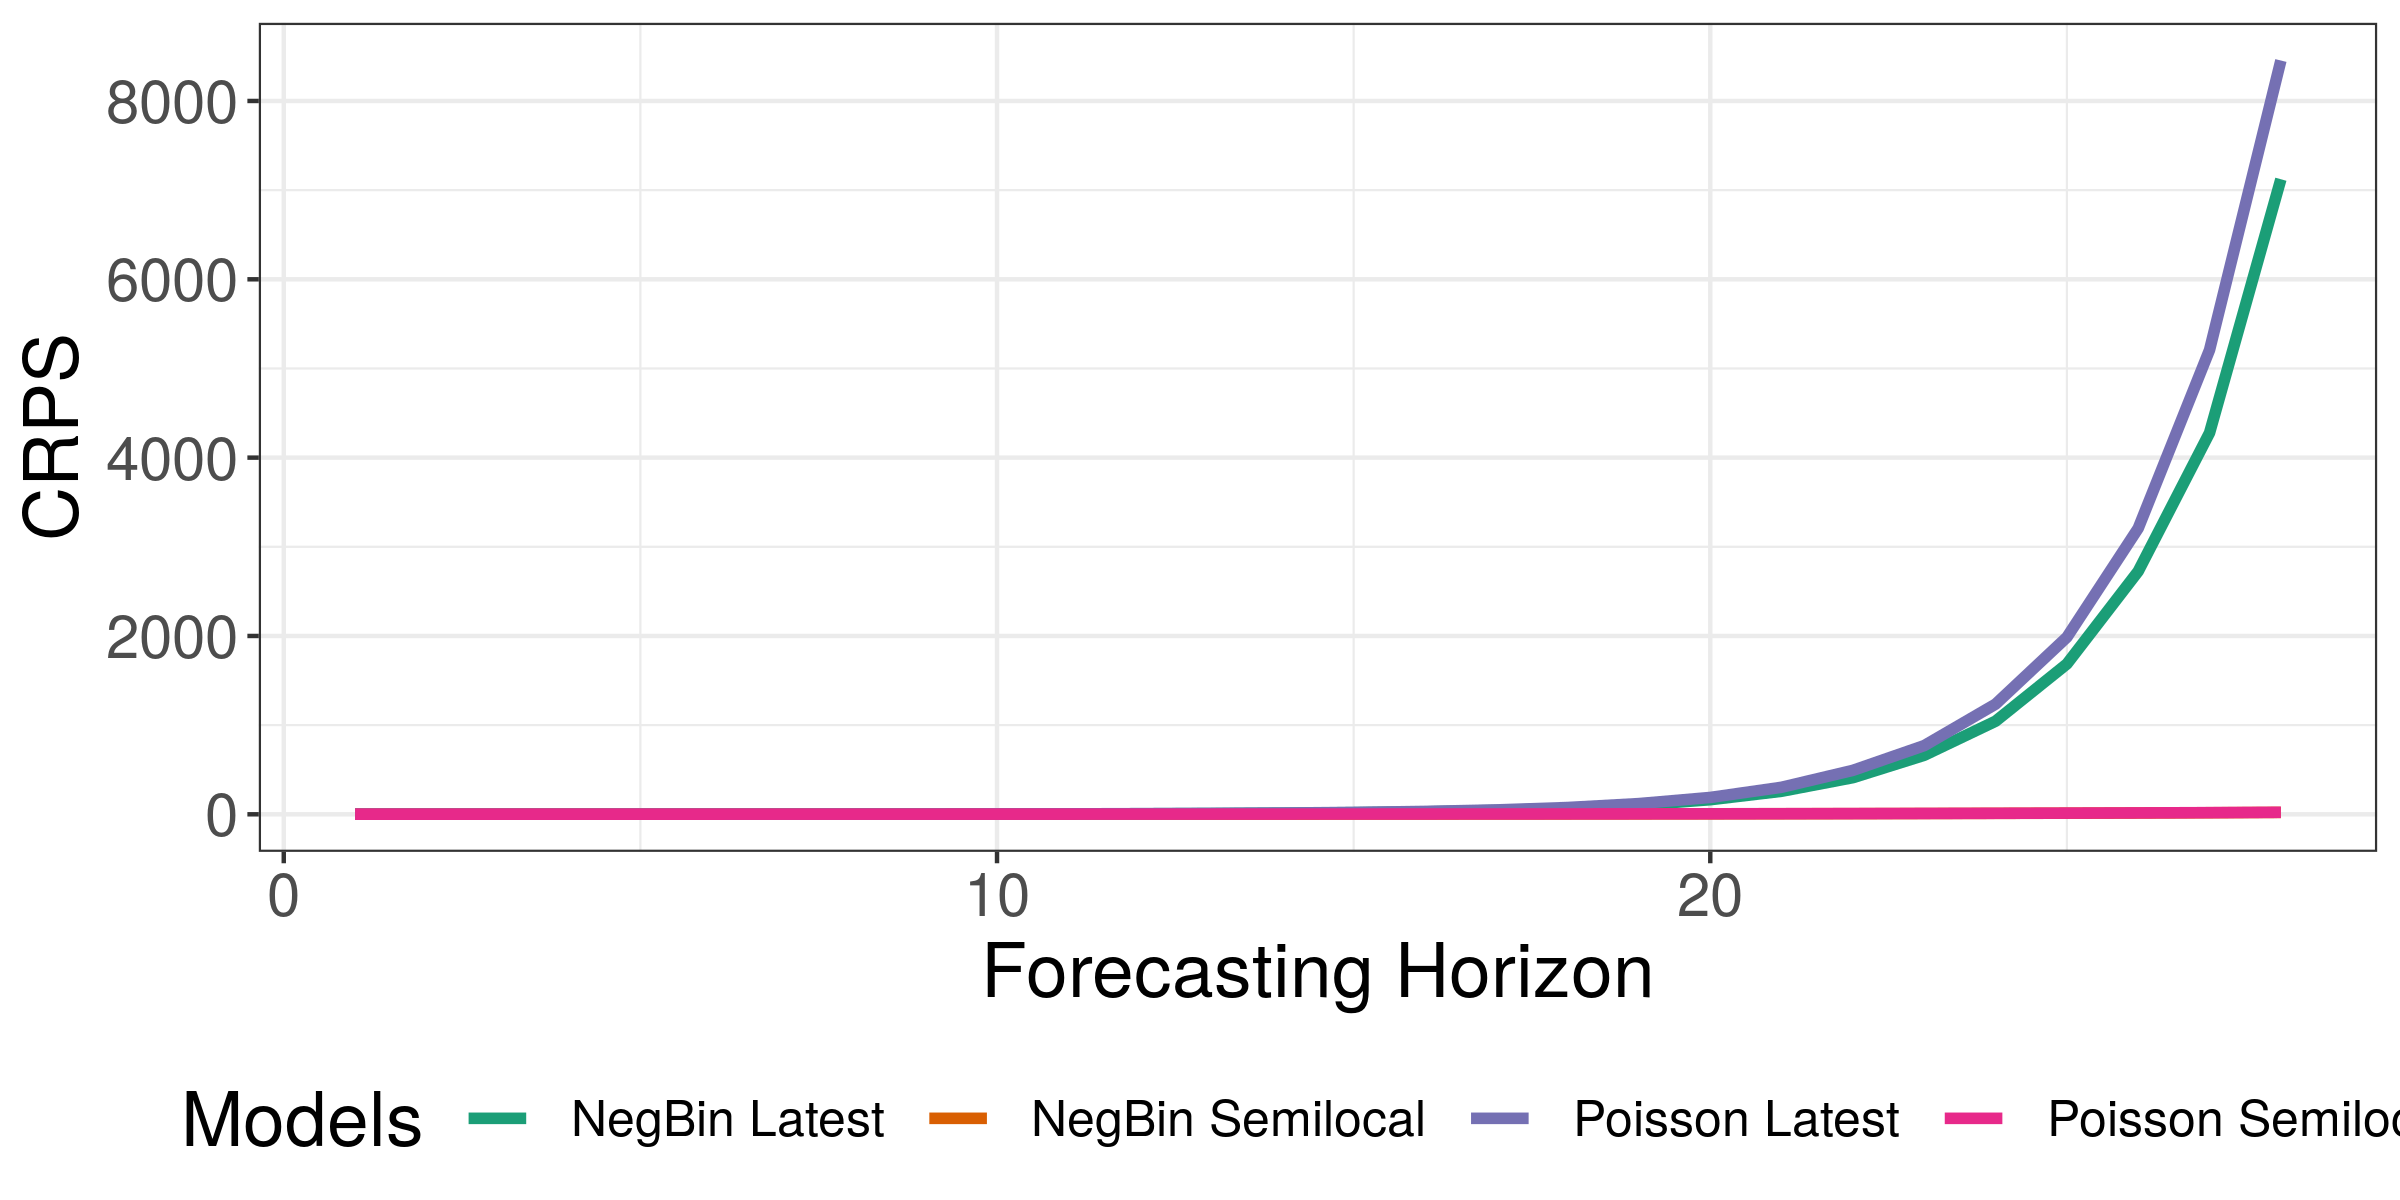
\includegraphics[width=\linewidth]{../output/Katwa_crps.png}  
  \caption{Contineously Ranked Probability Score}
  \label{fig:sub-first}
\end{subfigure}
\begin{subfigure}{0.5\textwidth}
  \centering
  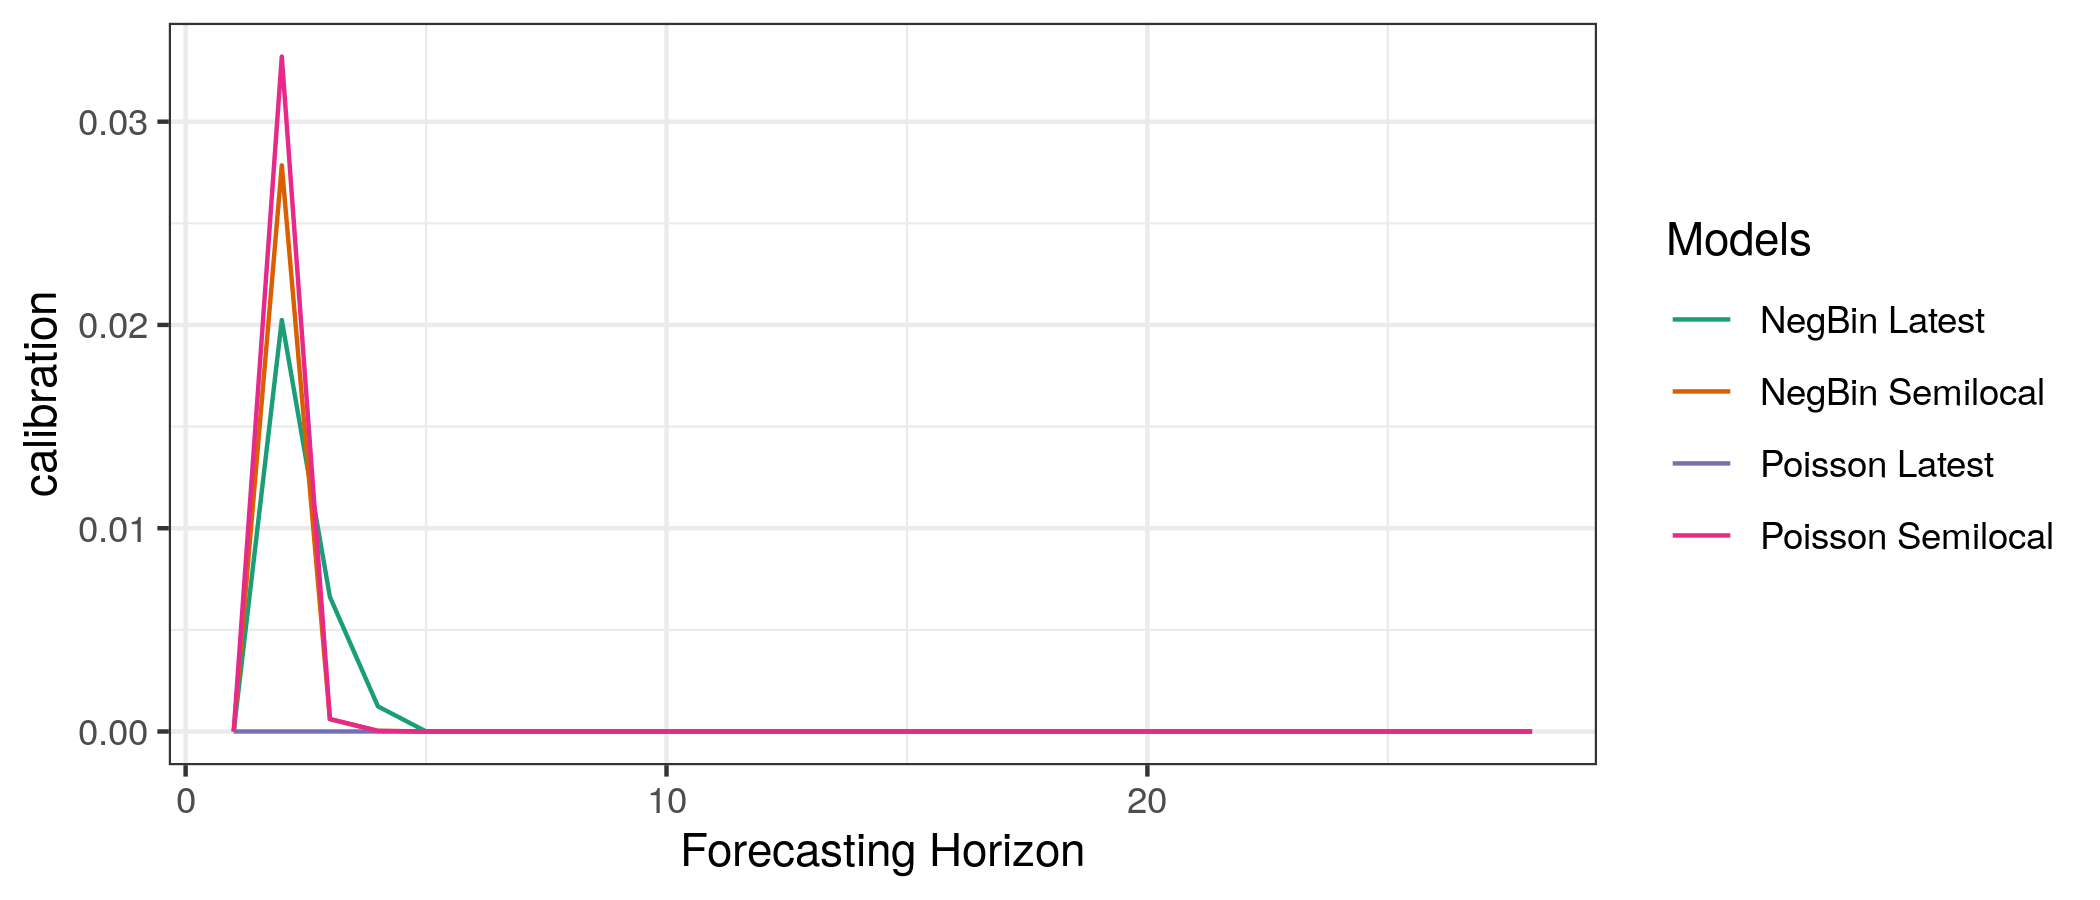
\includegraphics[width=\linewidth]{../output/Katwa_calibration.png}  
  \caption{Calibration p-value}
  \label{fig:sub-second}
\end{subfigure}

\begin{subfigure}{0.5\textwidth}
  \centering
  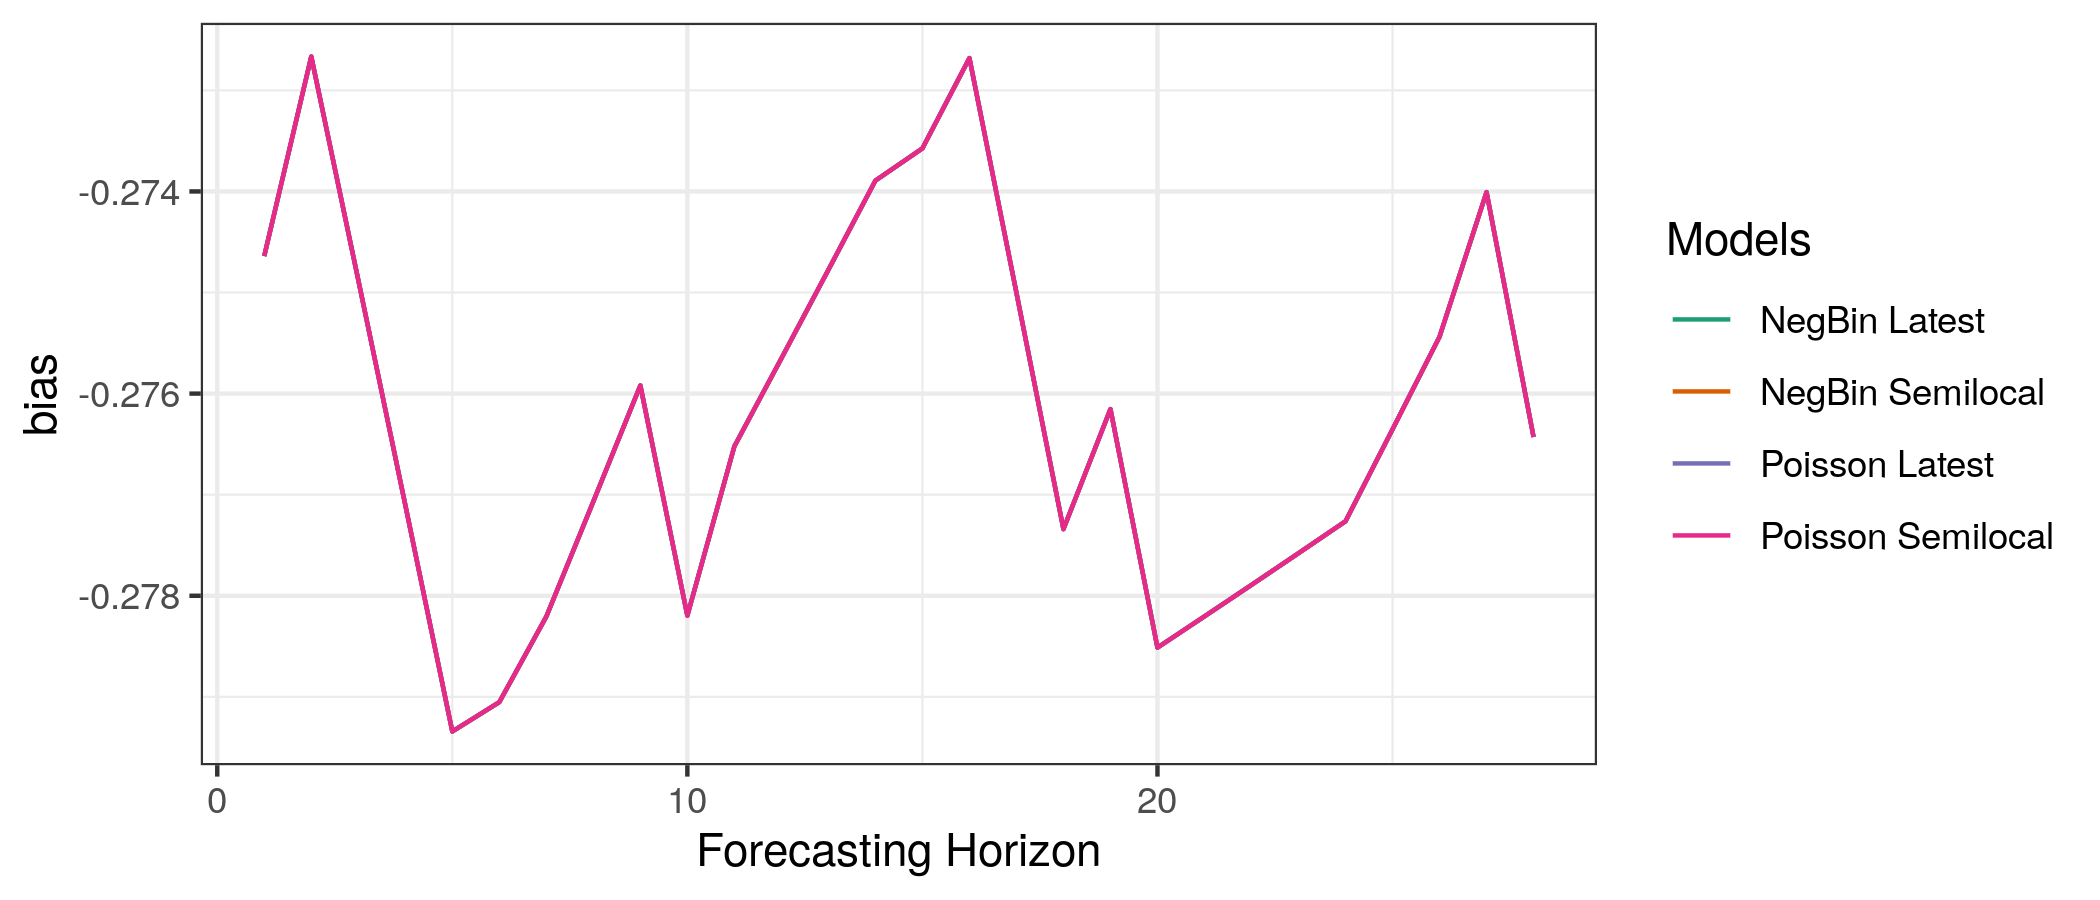
\includegraphics[width=\linewidth]{../output/Katwa_bias.png}  
  \caption{Bias}
  \label{fig:sub-third}
\end{subfigure}
\begin{subfigure}{0.5\textwidth}
  \centering
  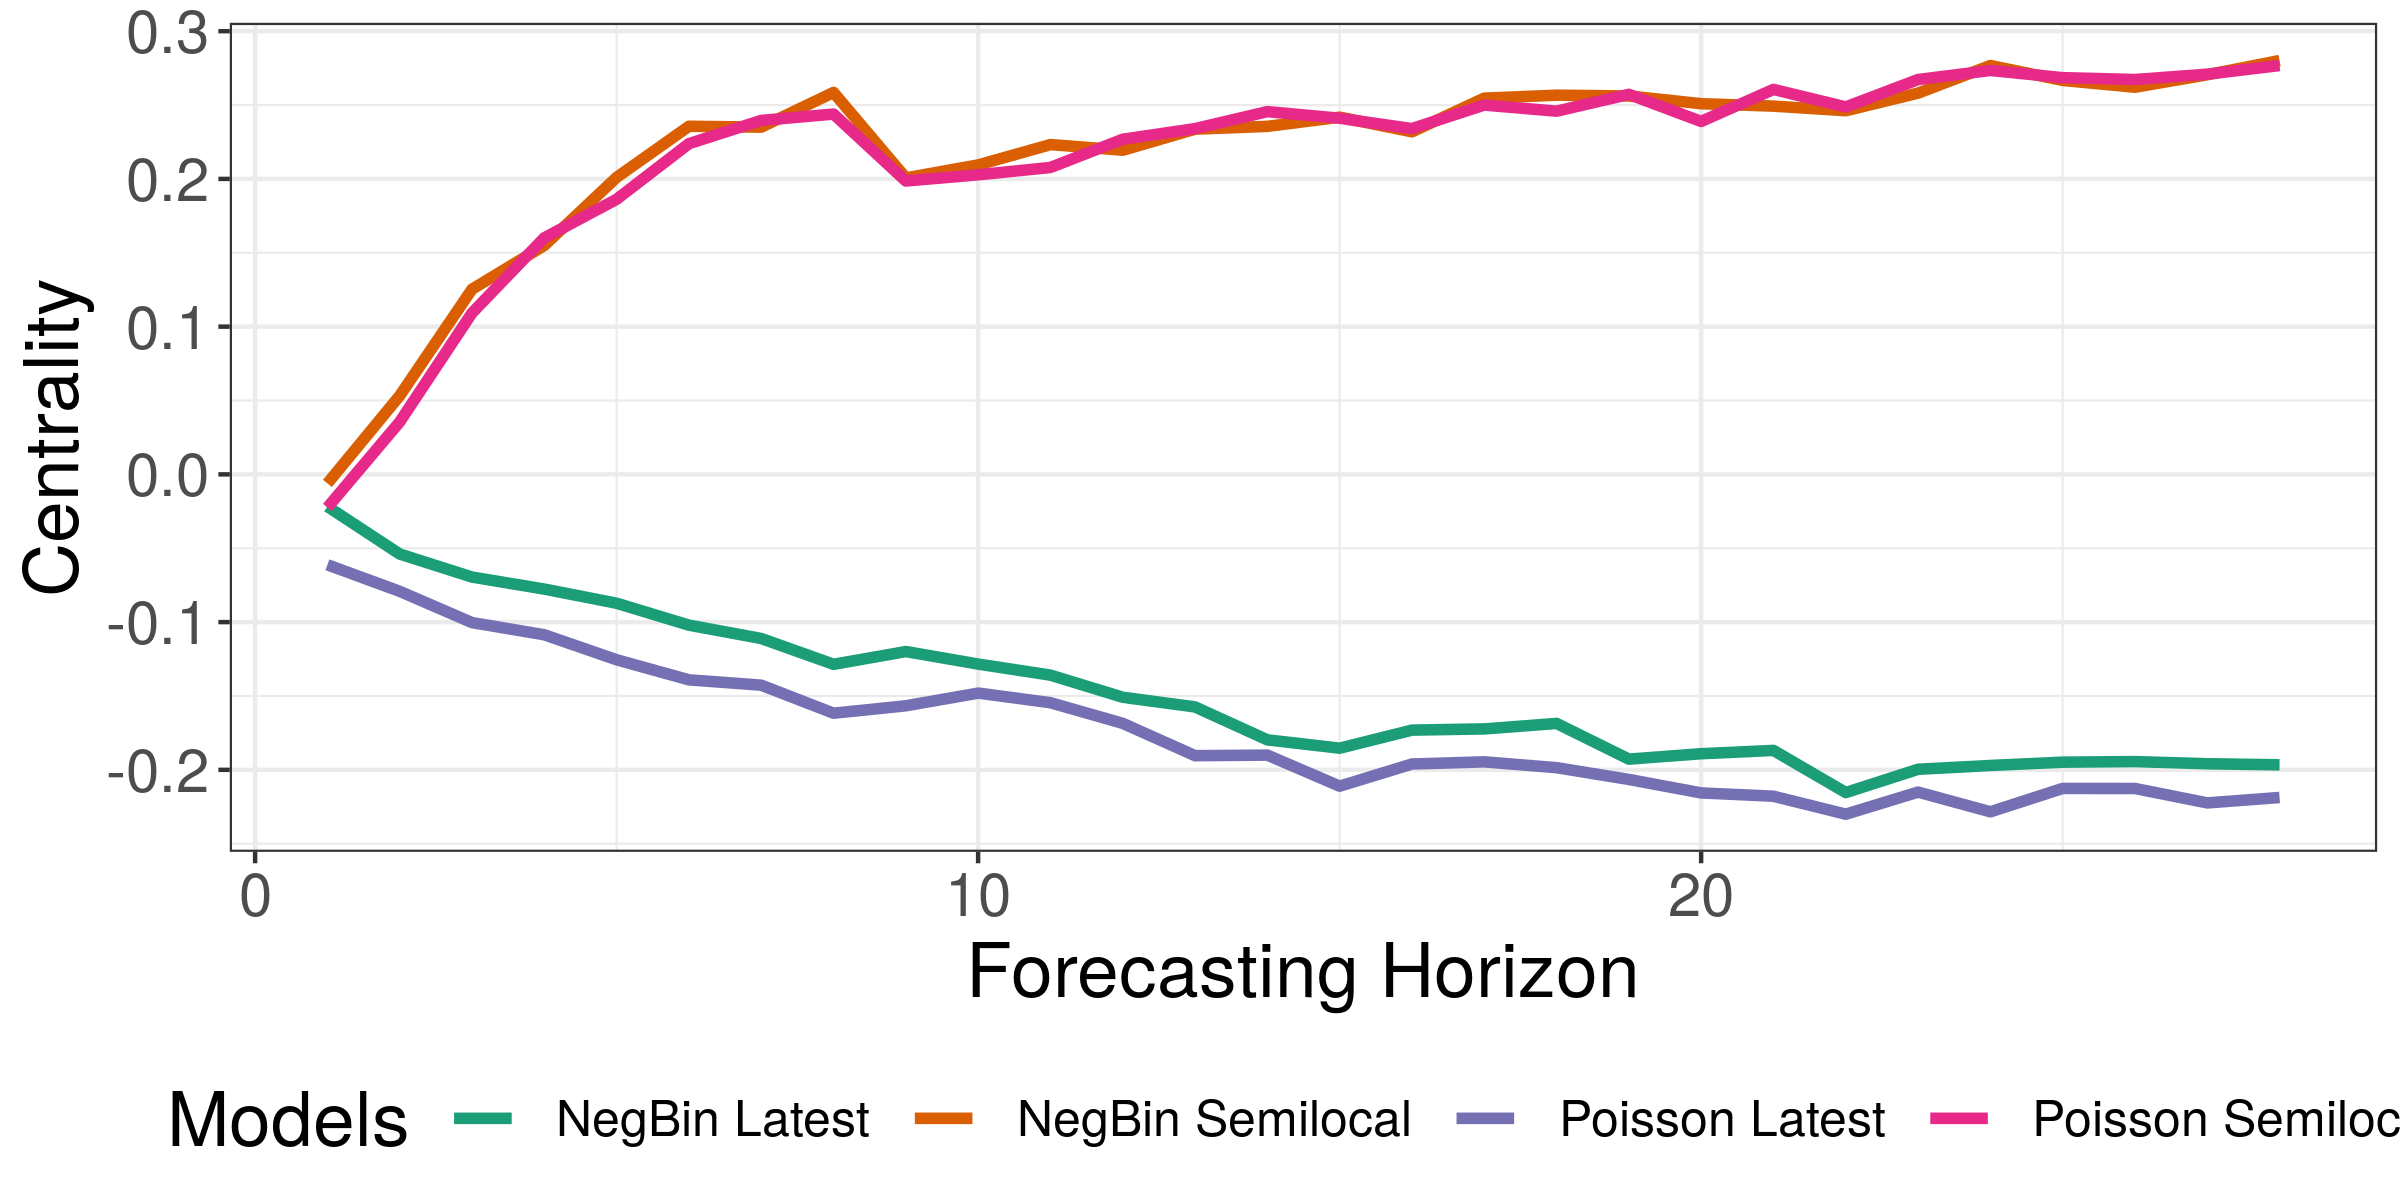
\includegraphics[width=\linewidth]{../output/Katwa_centrality.png}  
  \caption{Centrality of PIT values}
  \label{fig:nat_scores_4}
\end{subfigure}
  \caption{Scores for the entire outbreak as a function of the forecasting horizon.}

  \label{fig:nat_scores}
\end{figure}
 \section{ Kayina }\begin{figure}[H]\begin{subfigure}{\textwidth}  \centering  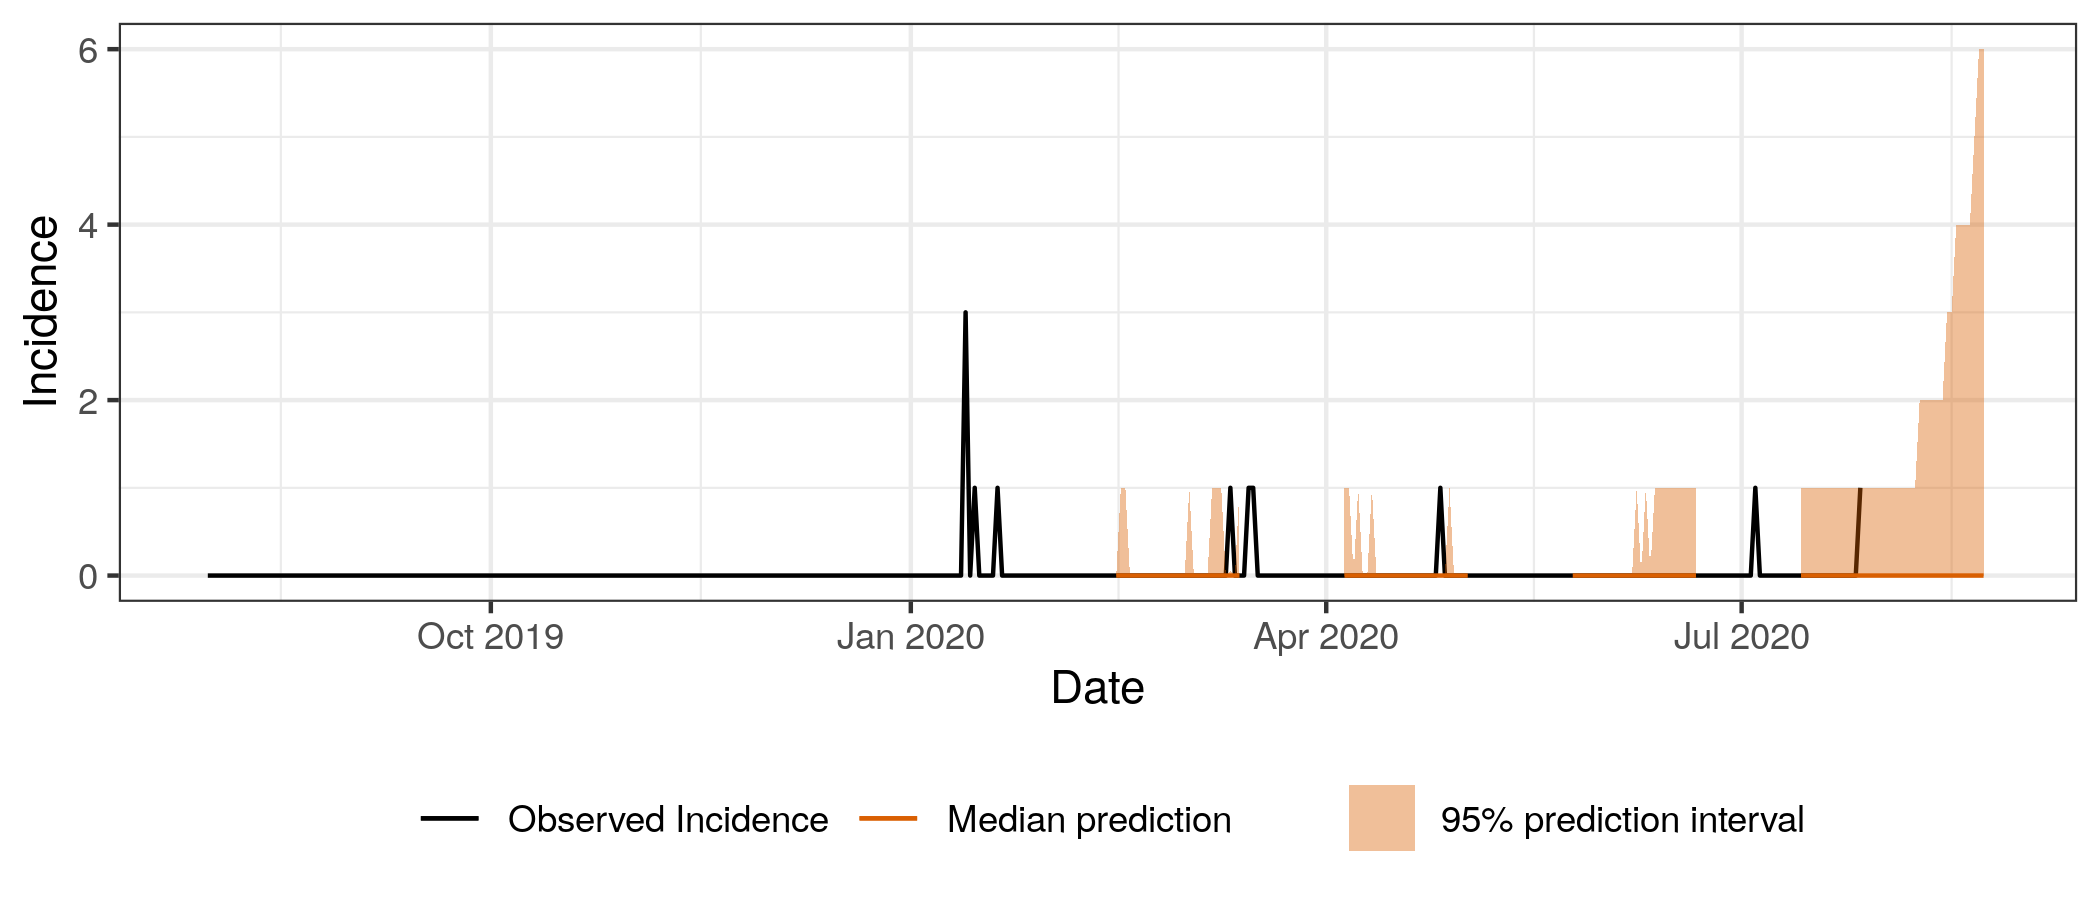
\includegraphics[width=0.9\linewidth, height=7cm]{../output/Kayina_predictions.png}  \caption{Forecasted and predicted incidence for the semilocal poisson model}\end{subfigure}

\begin{subfigure}{\textwidth}  \centering  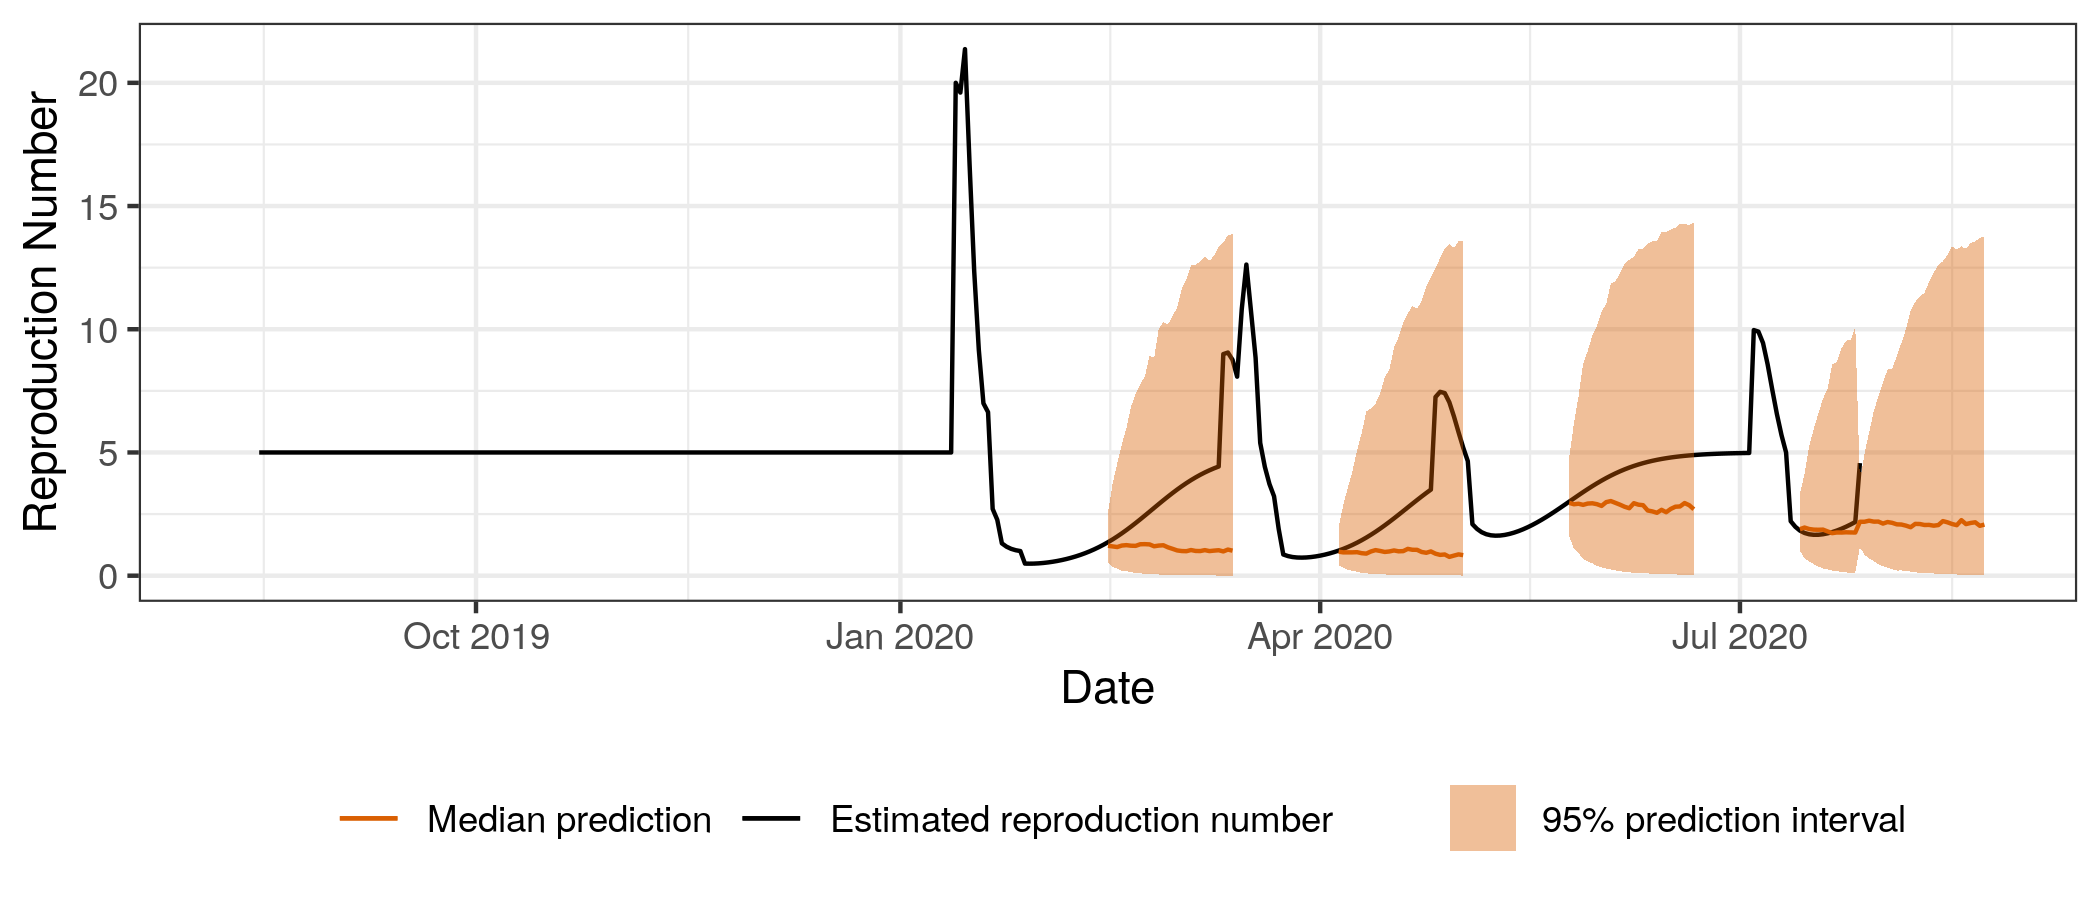
\includegraphics[width=0.9\linewidth, height=7cm]{../output/Kayina_Rs.png}  \caption{Forecasted and predicted repreoduction numbers for the semilocal poisson model}\end{subfigure}  \caption{Median forecast with 95 \% prediction intervals and observed values for incidence and reproduction number for the semilocal poisson model for Kayina.}\end{figure}

\begin{figure}[H]
\begin{subfigure}{0.5\textwidth}
  \centering
  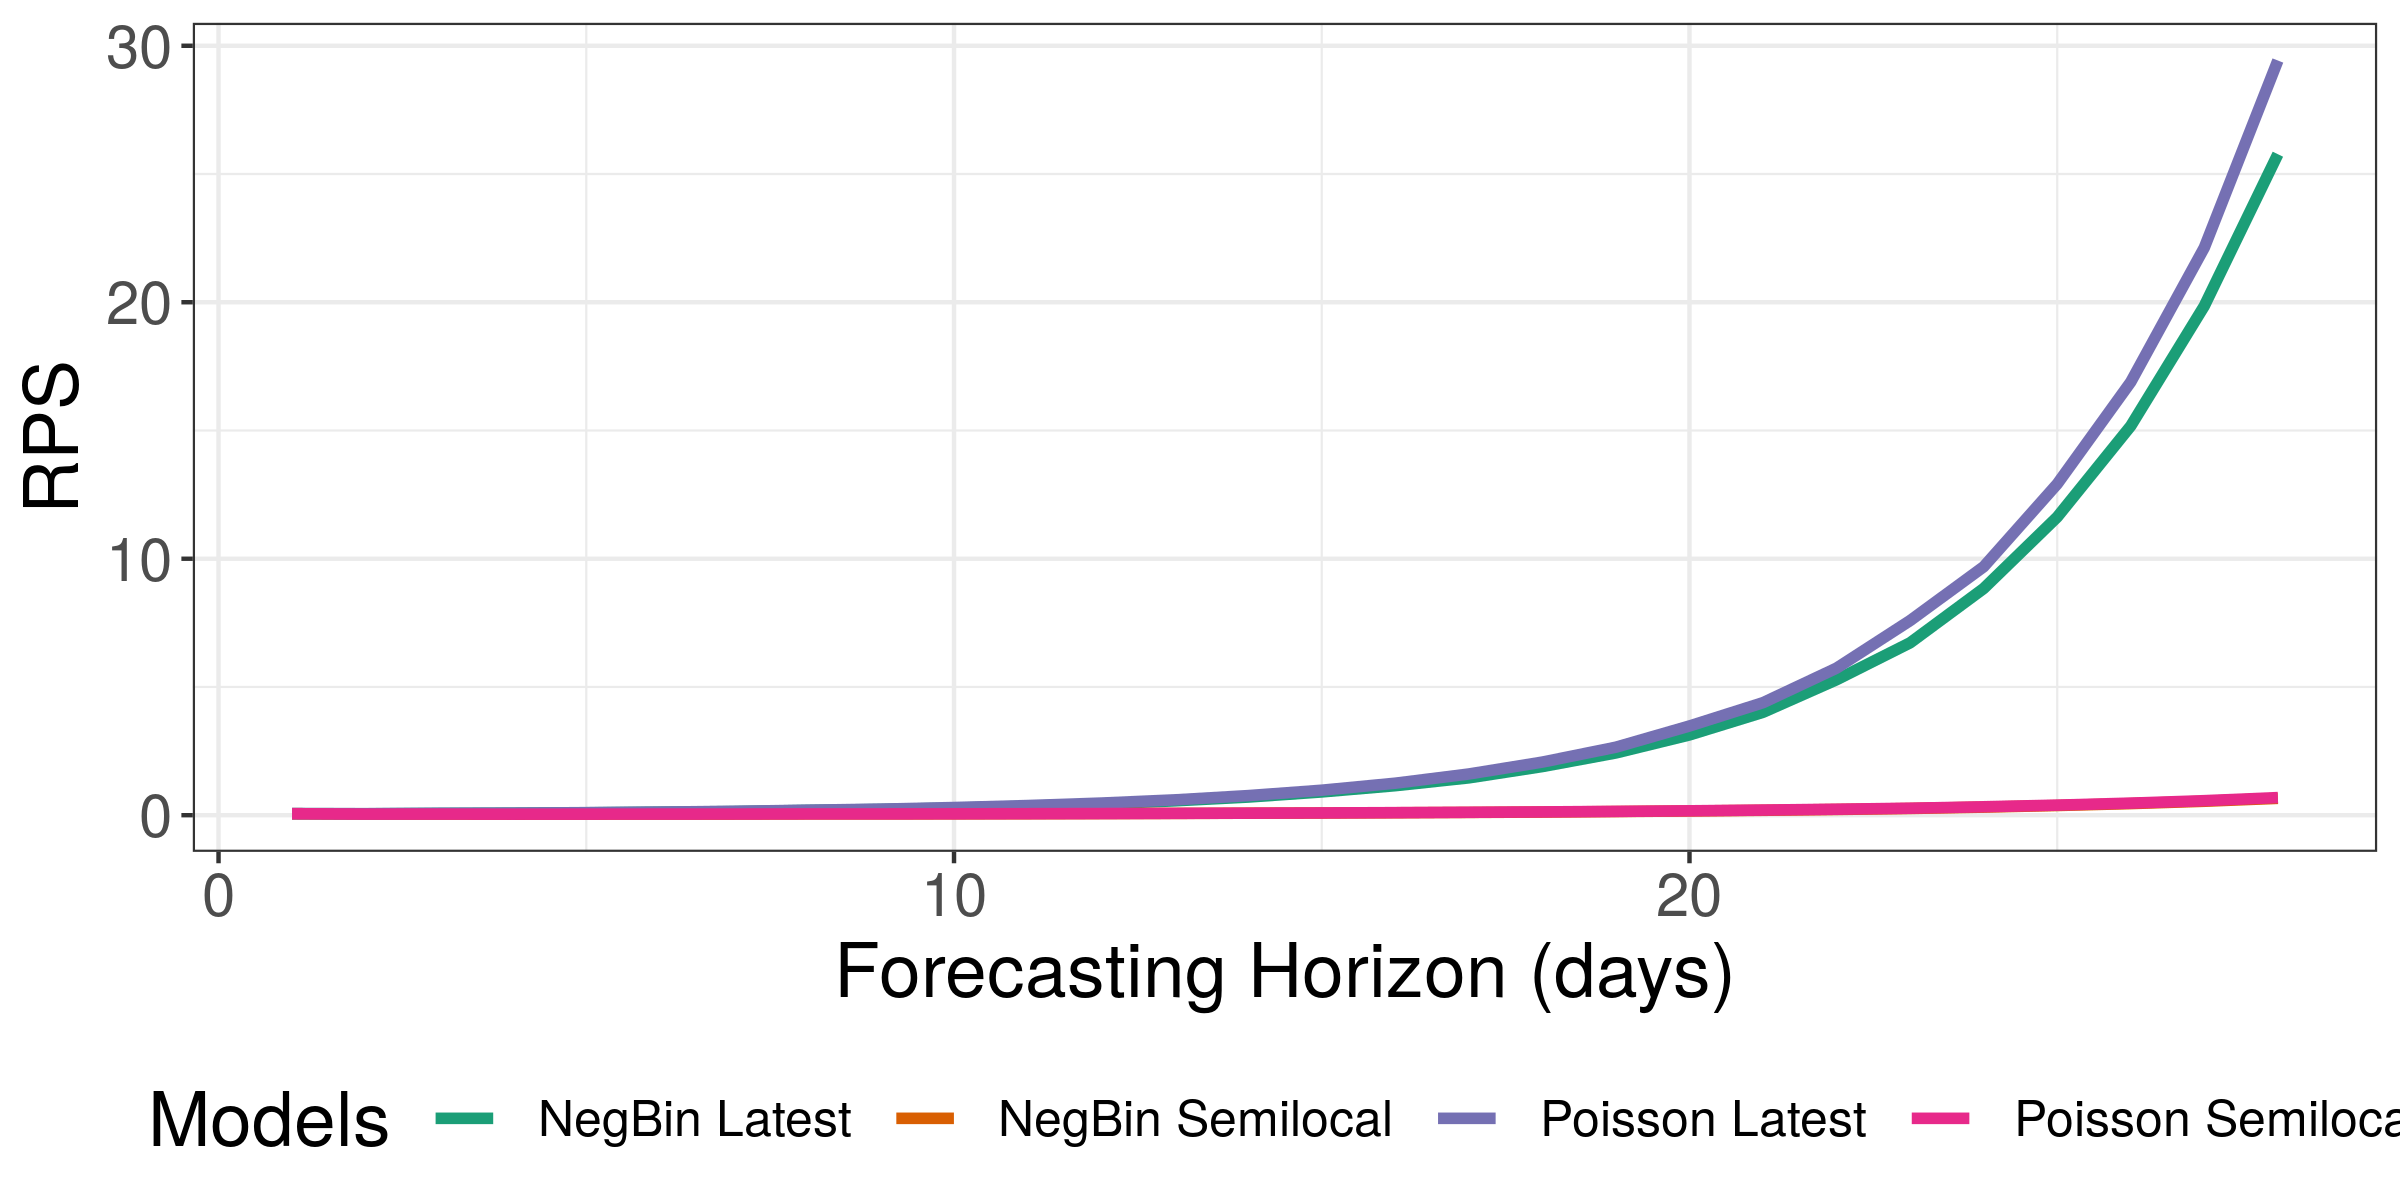
\includegraphics[width=\linewidth]{../output/Kayina_crps.png}  
  \caption{Contineously Ranked Probability Score}
  \label{fig:sub-first}
\end{subfigure}
\begin{subfigure}{0.5\textwidth}
  \centering
  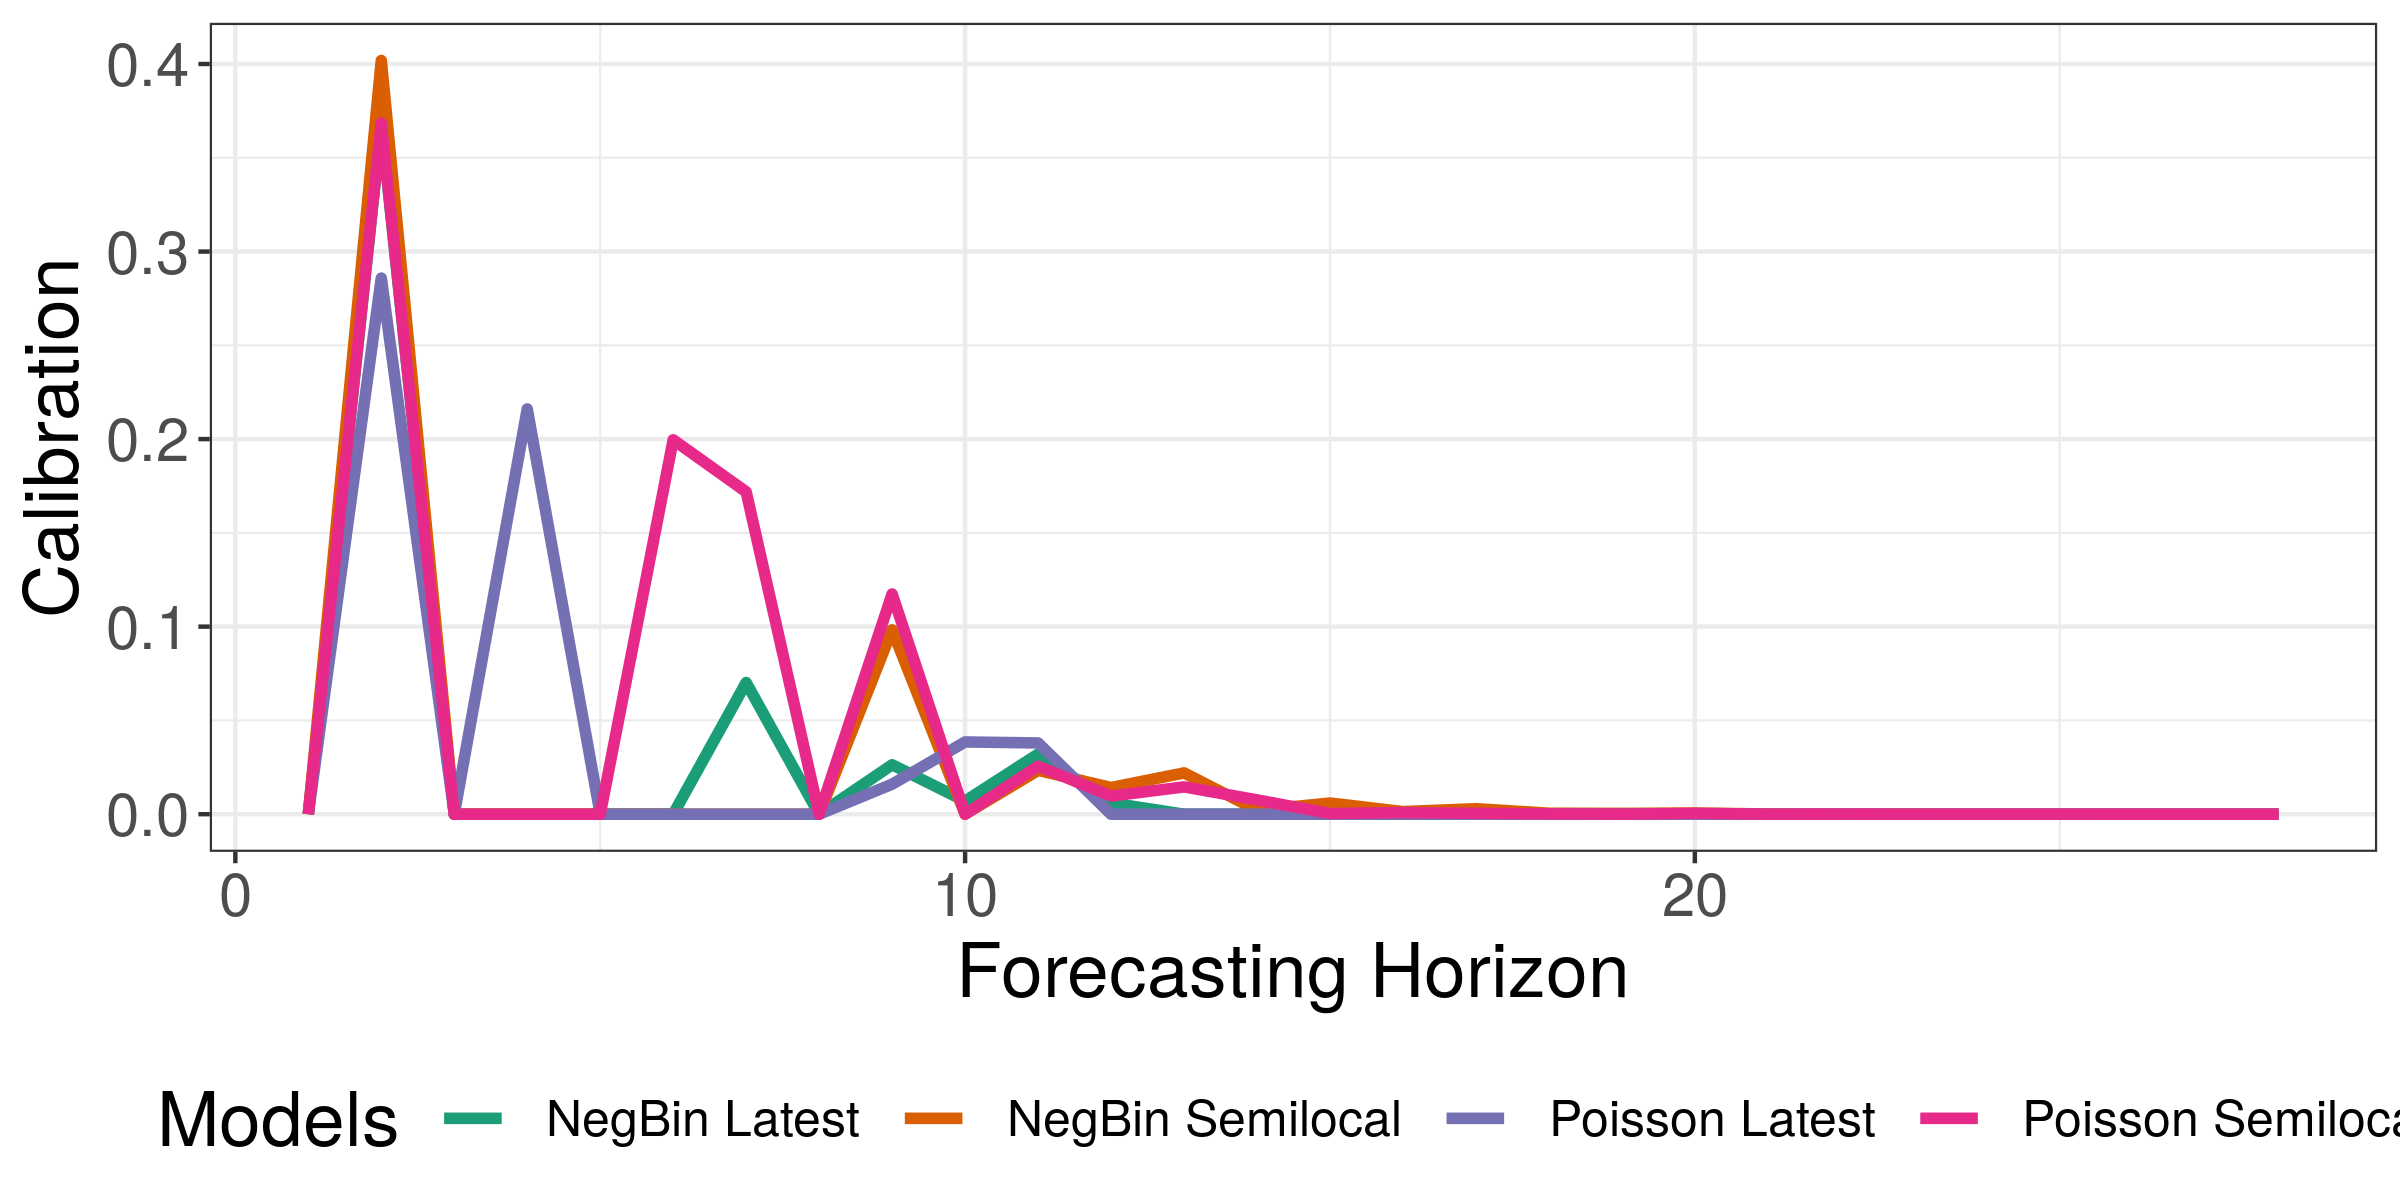
\includegraphics[width=\linewidth]{../output/Kayina_calibration.png}  
  \caption{Calibration p-value}
  \label{fig:sub-second}
\end{subfigure}

\begin{subfigure}{0.5\textwidth}
  \centering
  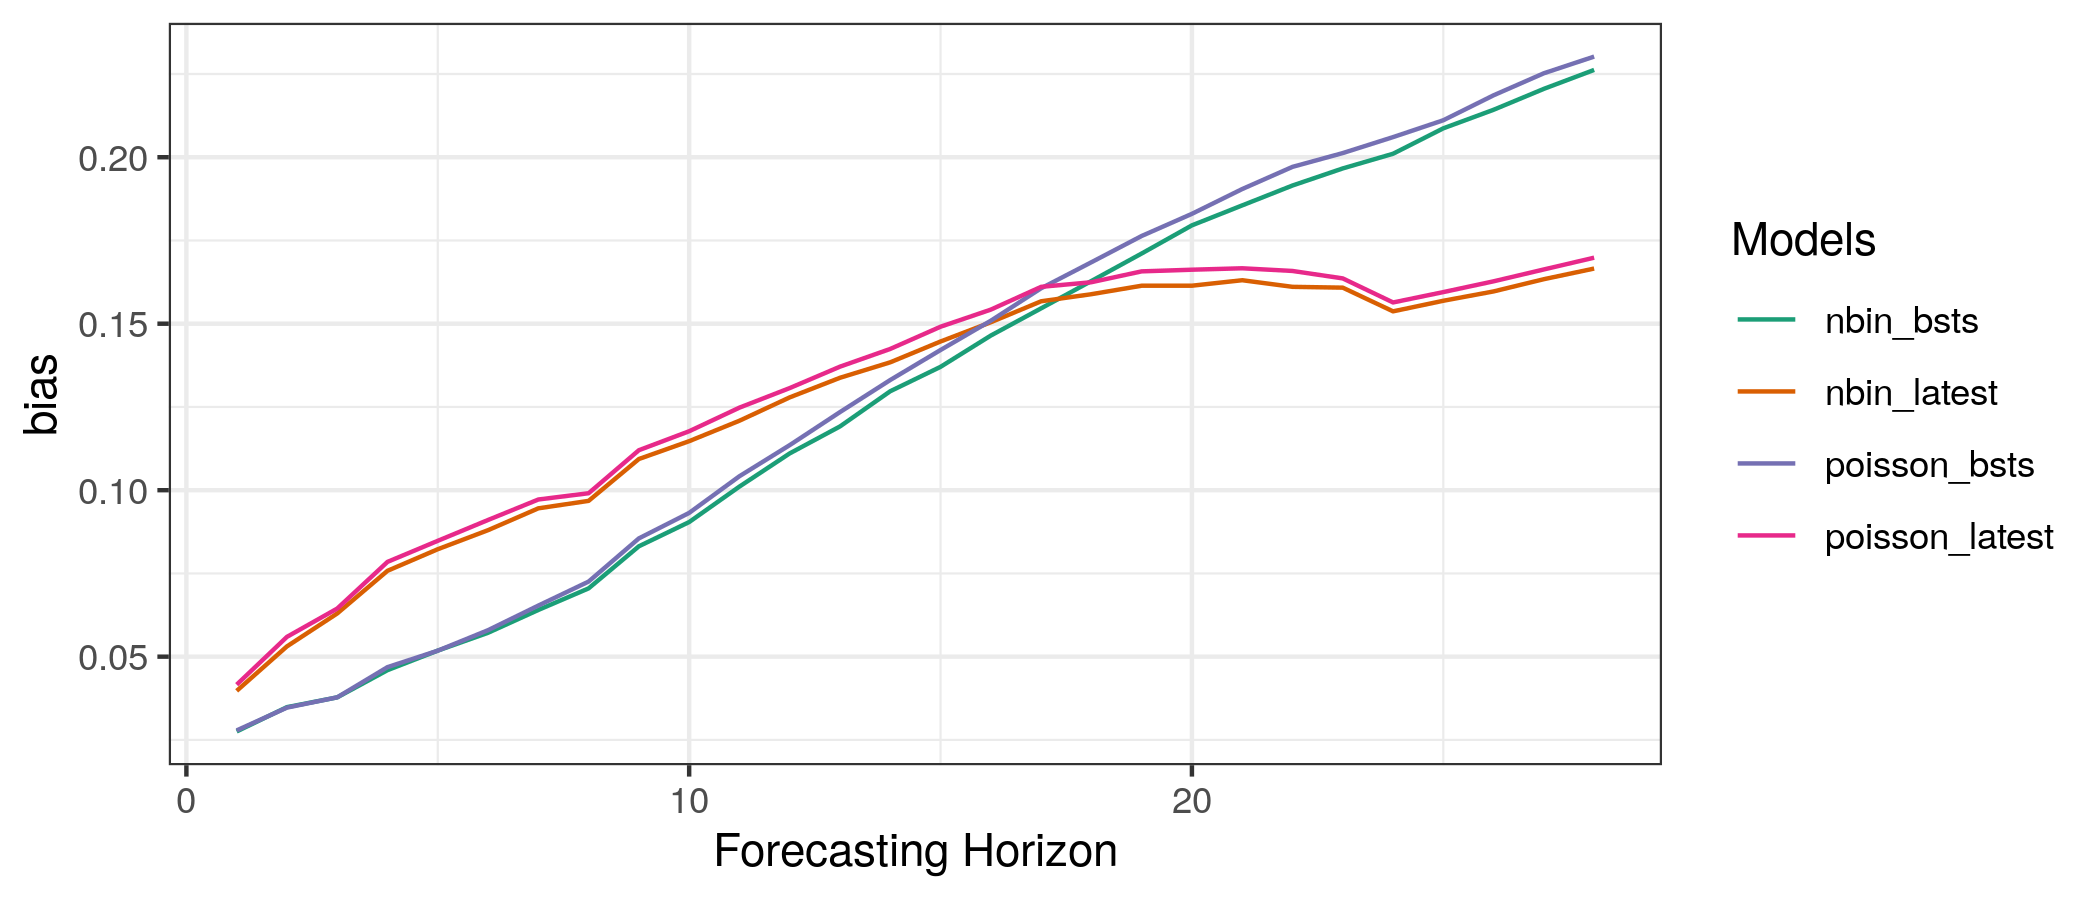
\includegraphics[width=\linewidth]{../output/Kayina_bias.png}  
  \caption{Bias}
  \label{fig:sub-third}
\end{subfigure}
\begin{subfigure}{0.5\textwidth}
  \centering
  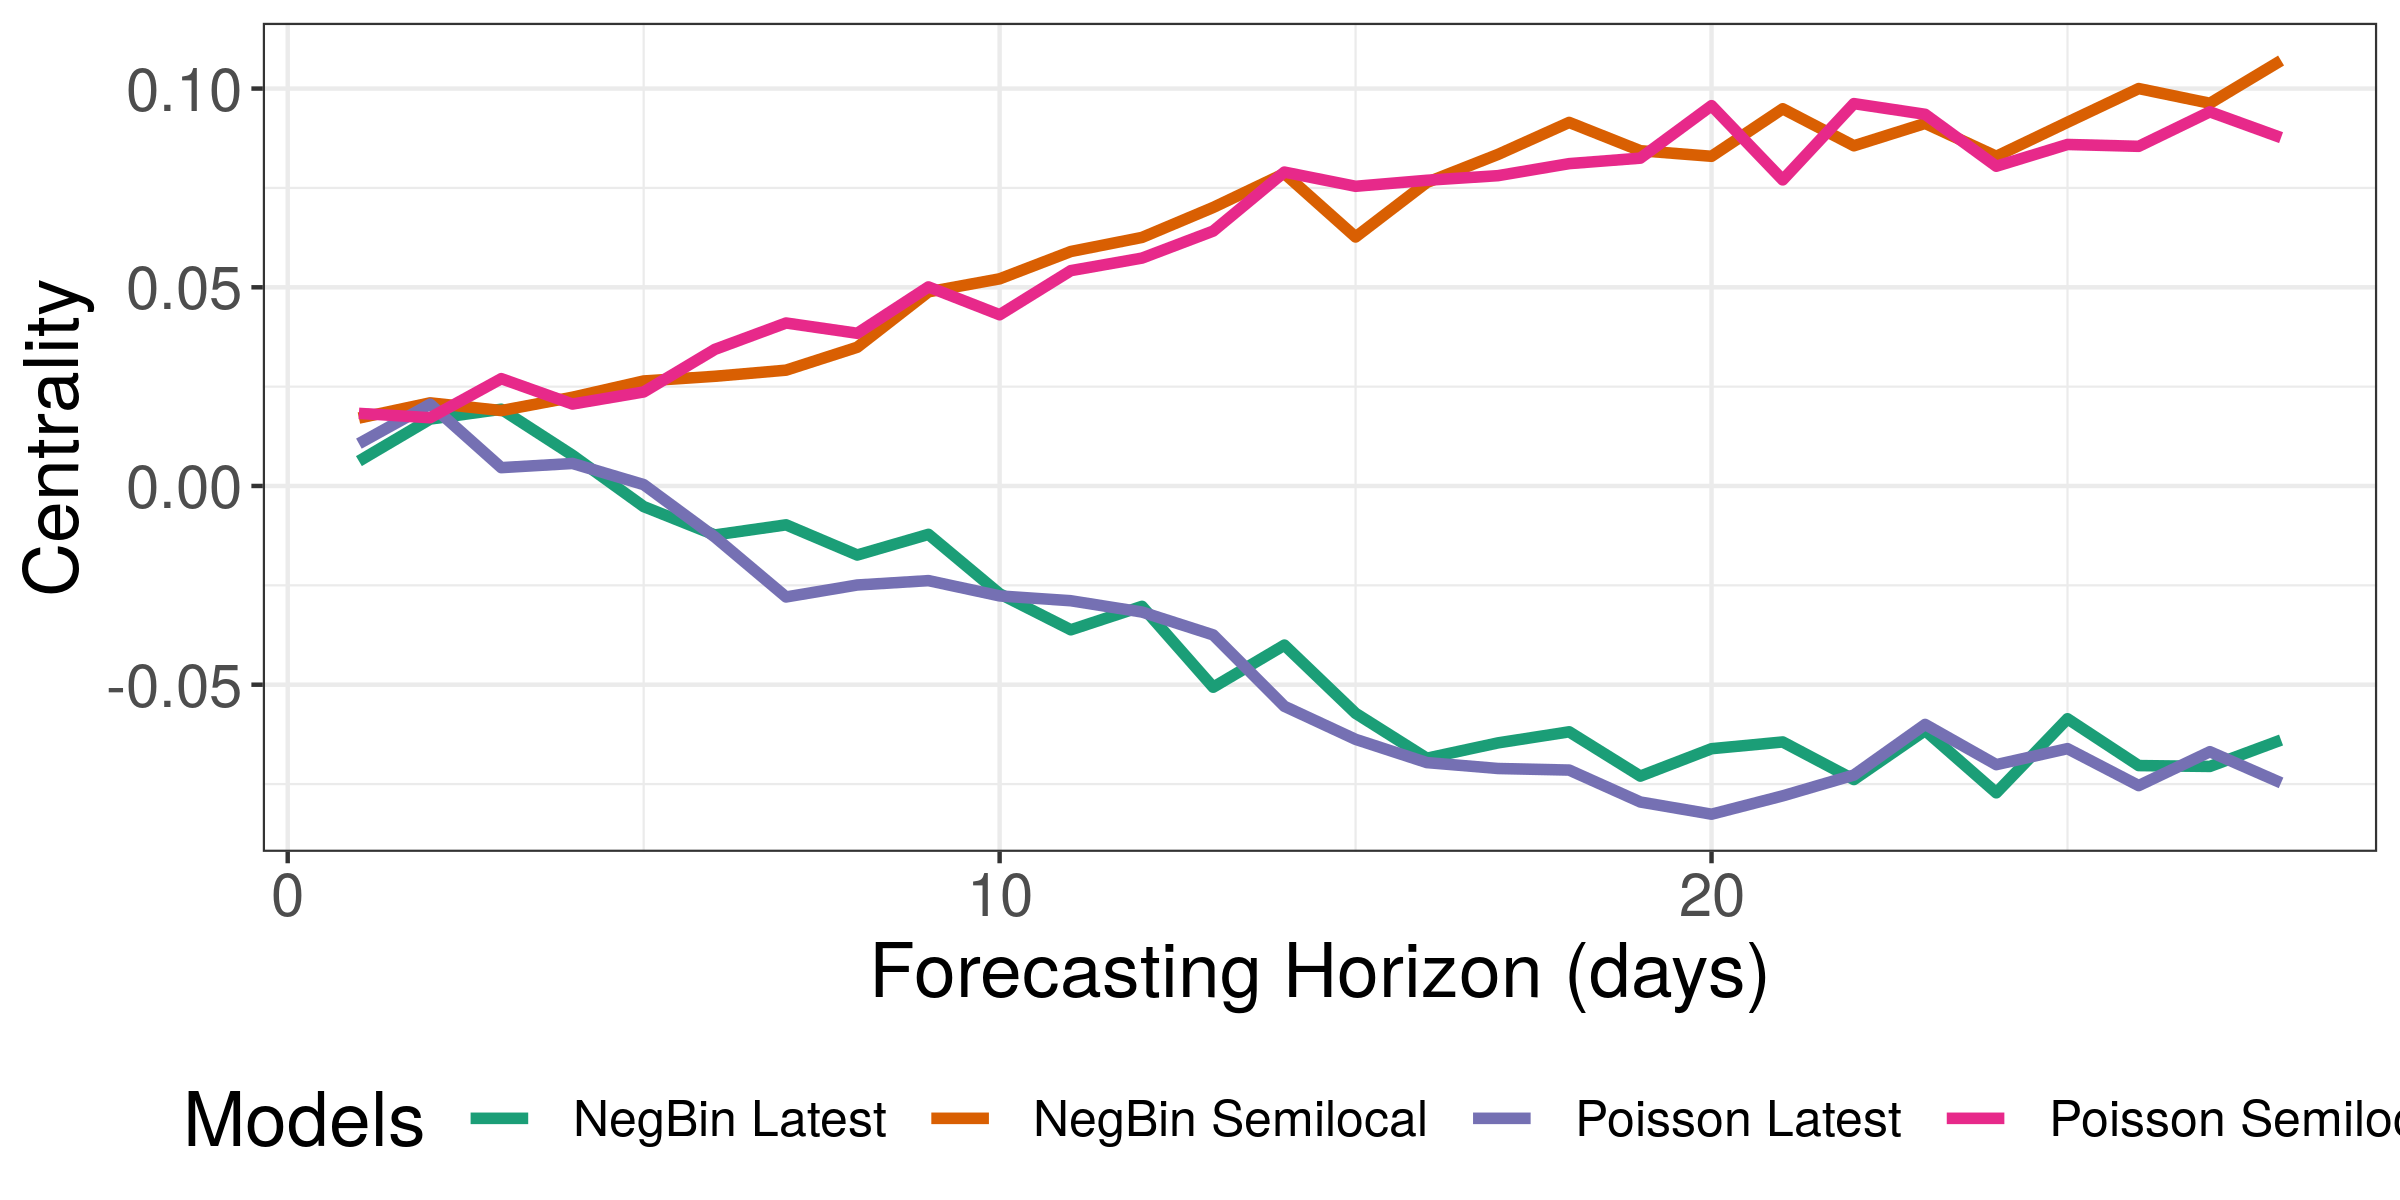
\includegraphics[width=\linewidth]{../output/Kayina_centrality.png}  
  \caption{Centrality of PIT values}
  \label{fig:nat_scores_4}
\end{subfigure}
  \caption{Scores for the entire outbreak as a function of the forecasting horizon.}

  \label{fig:nat_scores}
\end{figure}
 \section{ Kayna }\begin{figure}[H]\begin{subfigure}{\textwidth}  \centering  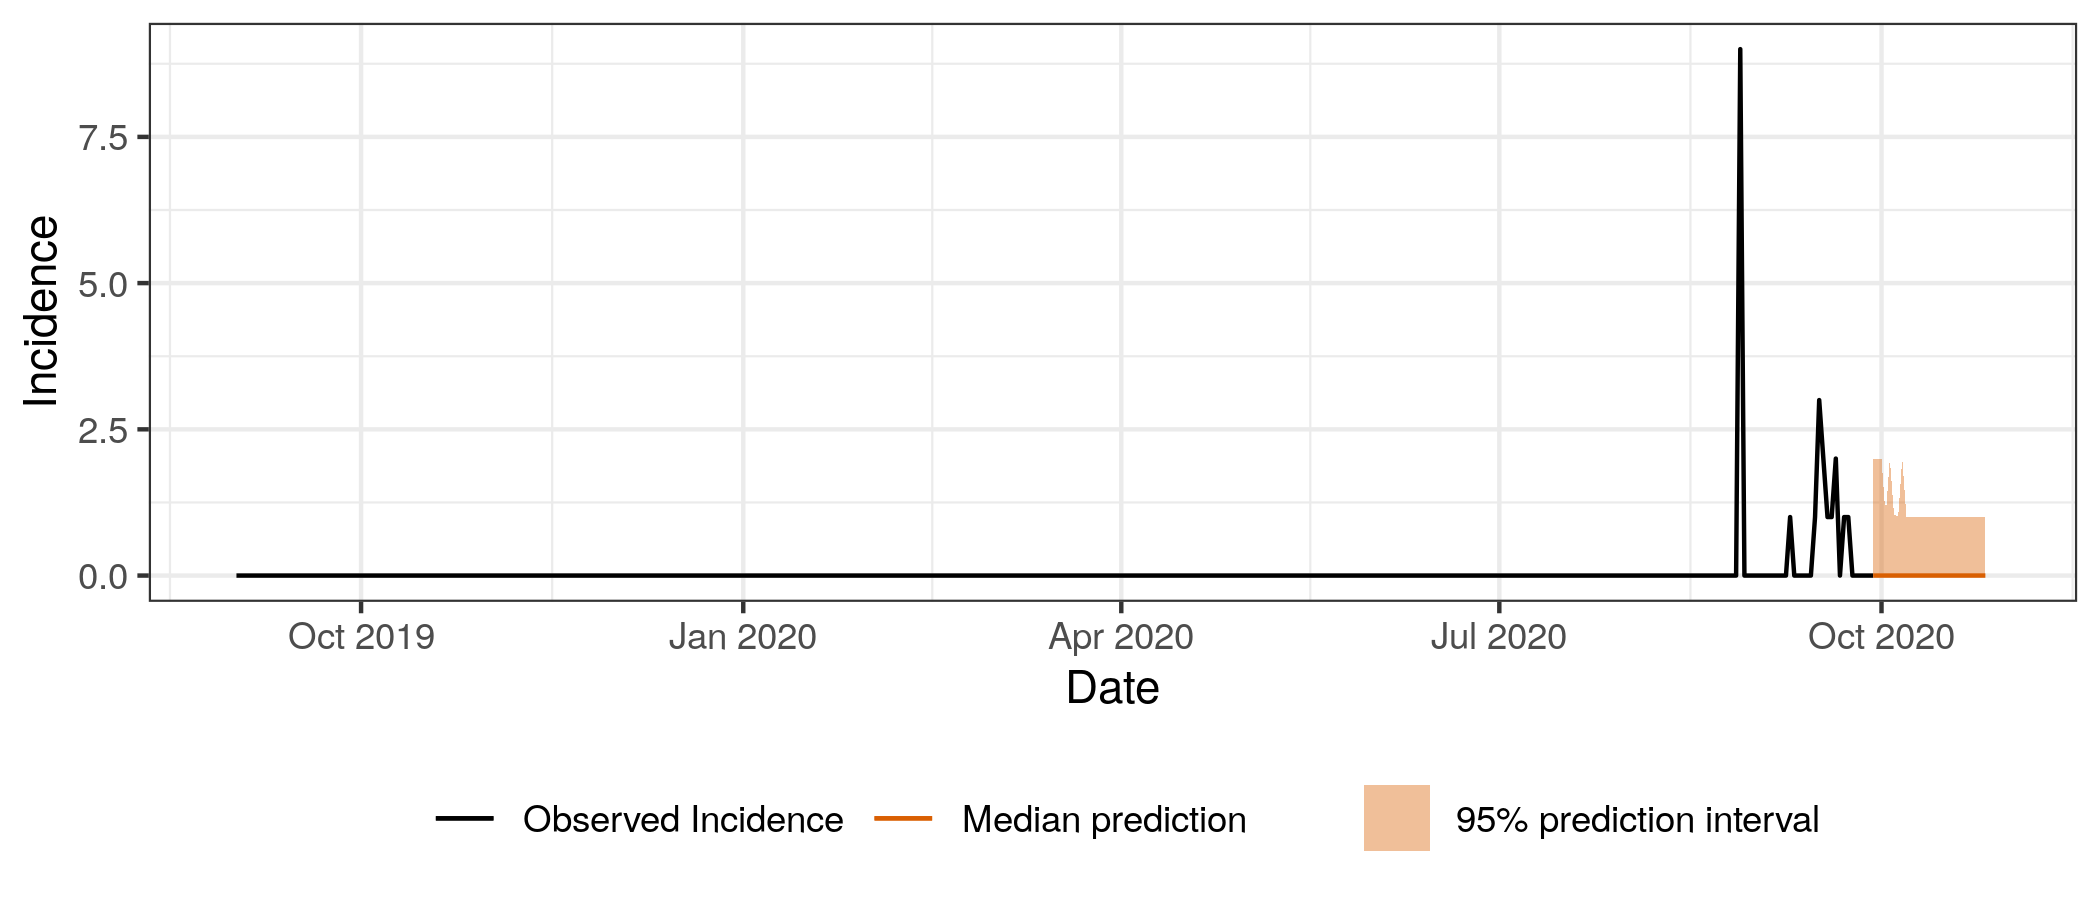
\includegraphics[width=0.9\linewidth, height=7cm]{../output/Kayna_predictions.png}  \caption{Forecasted and predicted incidence for the semilocal poisson model}\end{subfigure}

\begin{subfigure}{\textwidth}  \centering  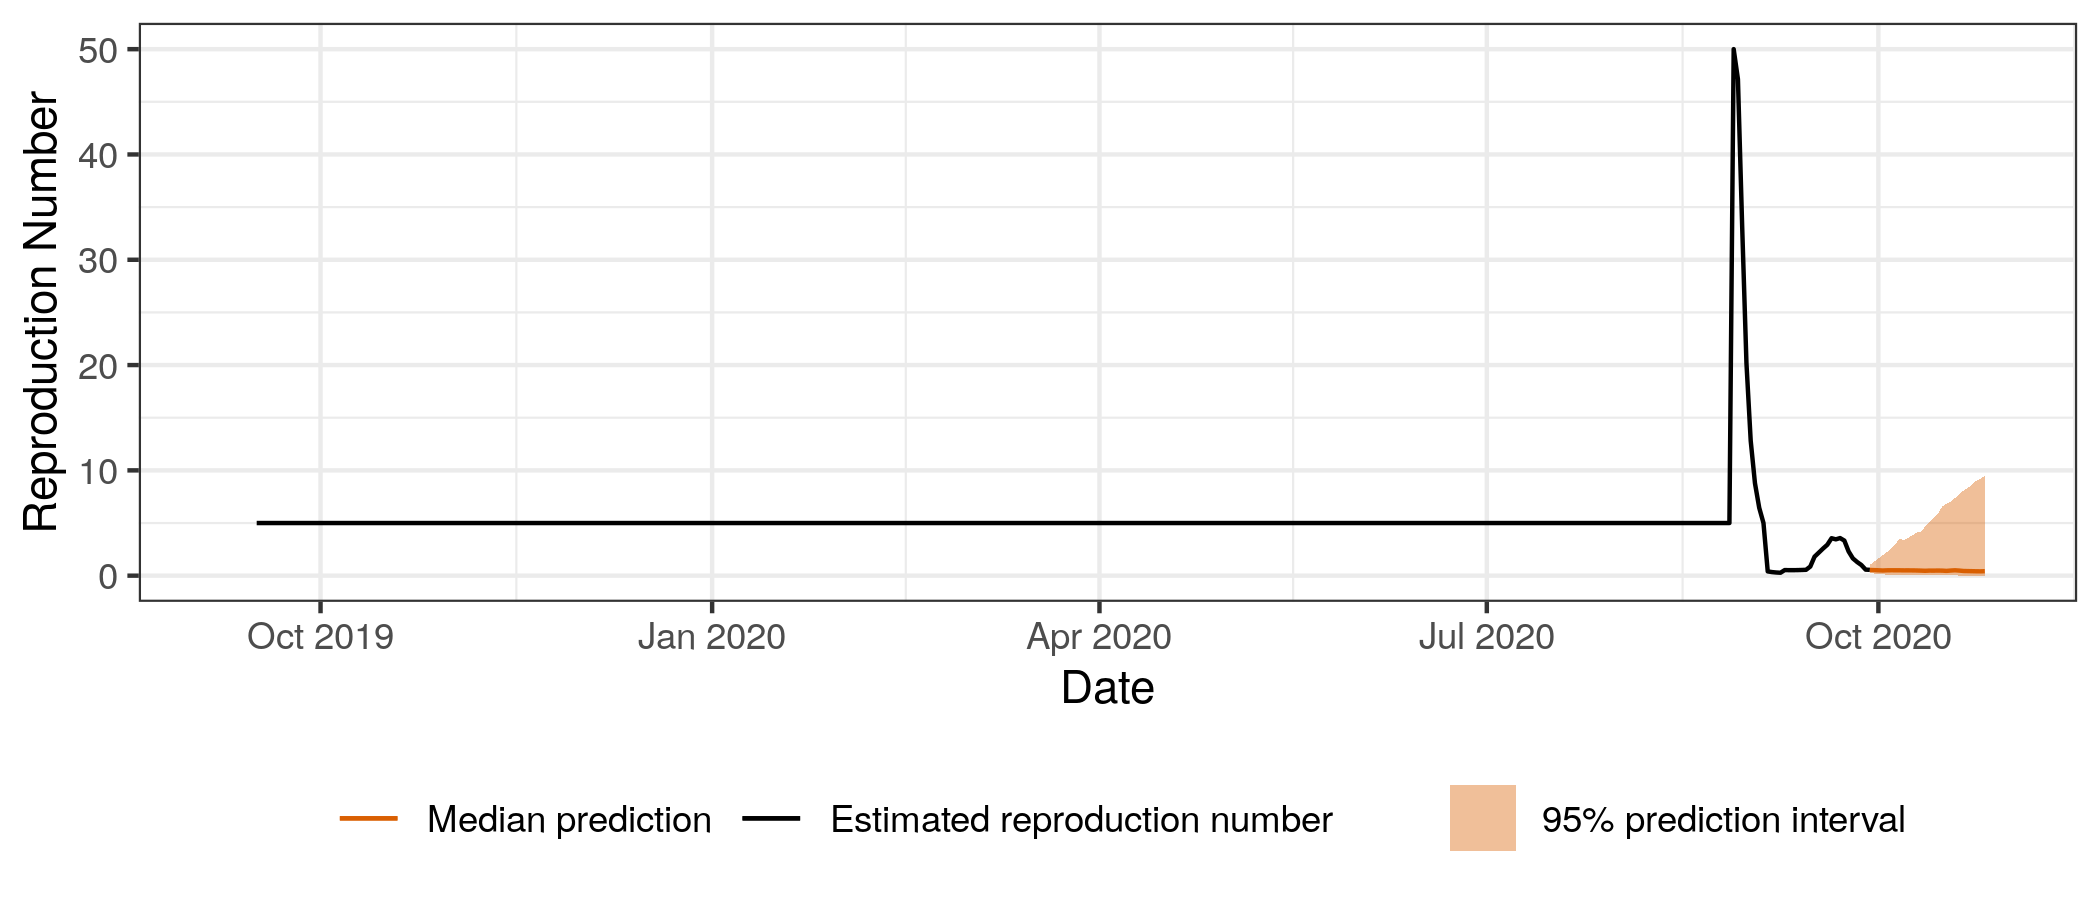
\includegraphics[width=0.9\linewidth, height=7cm]{../output/Kayna_Rs.png}  \caption{Forecasted and predicted repreoduction numbers for the semilocal poisson model}\end{subfigure}  \caption{Median forecast with 95 \% prediction intervals and observed values for incidence and reproduction number for the semilocal poisson model for Kayna.}\end{figure}

\begin{figure}[H]
\begin{subfigure}{0.5\textwidth}
  \centering
  \includegraphics[width=\linewidth]{../output/Kayna_crps.png}  
  \caption{Contineously Ranked Probability Score}
  \label{fig:sub-first}
\end{subfigure}
\begin{subfigure}{0.5\textwidth}
  \centering
  \includegraphics[width=\linewidth]{../output/Kayna_calibration.png}  
  \caption{Calibration p-value}
  \label{fig:sub-second}
\end{subfigure}

\begin{subfigure}{0.5\textwidth}
  \centering
  \includegraphics[width=\linewidth]{../output/Kayna_bias.png}  
  \caption{Bias}
  \label{fig:sub-third}
\end{subfigure}
\begin{subfigure}{0.5\textwidth}
  \centering
  \includegraphics[width=\linewidth]{../output/Kayna_centrality.png}  
  \caption{Centrality of PIT values}
  \label{fig:nat_scores_4}
\end{subfigure}
  \caption{Scores for the entire outbreak as a function of the forecasting horizon.}

  \label{fig:nat_scores}
\end{figure}
 \section{ Komanda }\begin{figure}[H]\begin{subfigure}{\textwidth}  \centering  \includegraphics[width=0.9\linewidth, height=7cm]{../output/Komanda_predictions.png}  \caption{Forecasted and predicted incidence for the semilocal poisson model}\end{subfigure}

\begin{subfigure}{\textwidth}  \centering  \includegraphics[width=0.9\linewidth, height=7cm]{../output/Komanda_Rs.png}  \caption{Forecasted and predicted repreoduction numbers for the semilocal poisson model}\end{subfigure}  \caption{Median forecast with 95 \% prediction intervals and observed values for incidence and reproduction number for the semilocal poisson model for Komanda.}\end{figure}

\begin{figure}[H]
\begin{subfigure}{0.5\textwidth}
  \centering
  \includegraphics[width=\linewidth]{../output/Komanda_crps.png}  
  \caption{Contineously Ranked Probability Score}
  \label{fig:sub-first}
\end{subfigure}
\begin{subfigure}{0.5\textwidth}
  \centering
  \includegraphics[width=\linewidth]{../output/Komanda_calibration.png}  
  \caption{Calibration p-value}
  \label{fig:sub-second}
\end{subfigure}

\begin{subfigure}{0.5\textwidth}
  \centering
  \includegraphics[width=\linewidth]{../output/Komanda_bias.png}  
  \caption{Bias}
  \label{fig:sub-third}
\end{subfigure}
\begin{subfigure}{0.5\textwidth}
  \centering
  \includegraphics[width=\linewidth]{../output/Komanda_centrality.png}  
  \caption{Centrality of PIT values}
  \label{fig:nat_scores_4}
\end{subfigure}
  \caption{Scores for the entire outbreak as a function of the forecasting horizon.}

  \label{fig:nat_scores}
\end{figure}
 \section{ Kyondo }\begin{figure}[H]\begin{subfigure}{\textwidth}  \centering  \includegraphics[width=0.9\linewidth, height=7cm]{../output/Kyondo_predictions.png}  \caption{Forecasted and predicted incidence for the semilocal poisson model}\end{subfigure}

\begin{subfigure}{\textwidth}  \centering  \includegraphics[width=0.9\linewidth, height=7cm]{../output/Kyondo_Rs.png}  \caption{Forecasted and predicted repreoduction numbers for the semilocal poisson model}\end{subfigure}  \caption{Median forecast with 95 \% prediction intervals and observed values for incidence and reproduction number for the semilocal poisson model for Kyondo.}\end{figure}

\begin{figure}[H]
\begin{subfigure}{0.5\textwidth}
  \centering
  \includegraphics[width=\linewidth]{../output/Kyondo_crps.png}  
  \caption{Contineously Ranked Probability Score}
  \label{fig:sub-first}
\end{subfigure}
\begin{subfigure}{0.5\textwidth}
  \centering
  \includegraphics[width=\linewidth]{../output/Kyondo_calibration.png}  
  \caption{Calibration p-value}
  \label{fig:sub-second}
\end{subfigure}

\begin{subfigure}{0.5\textwidth}
  \centering
  \includegraphics[width=\linewidth]{../output/Kyondo_bias.png}  
  \caption{Bias}
  \label{fig:sub-third}
\end{subfigure}
\begin{subfigure}{0.5\textwidth}
  \centering
  \includegraphics[width=\linewidth]{../output/Kyondo_centrality.png}  
  \caption{Centrality of PIT values}
  \label{fig:nat_scores_4}
\end{subfigure}
  \caption{Scores for the entire outbreak as a function of the forecasting horizon.}

  \label{fig:nat_scores}
\end{figure}
 \section{ Lolwa }\begin{figure}[H]\begin{subfigure}{\textwidth}  \centering  \includegraphics[width=0.9\linewidth, height=7cm]{../output/Lolwa_predictions.png}  \caption{Forecasted and predicted incidence for the semilocal poisson model}\end{subfigure}

\begin{subfigure}{\textwidth}  \centering  \includegraphics[width=0.9\linewidth, height=7cm]{../output/Lolwa_Rs.png}  \caption{Forecasted and predicted repreoduction numbers for the semilocal poisson model}\end{subfigure}  \caption{Median forecast with 95 \% prediction intervals and observed values for incidence and reproduction number for the semilocal poisson model for Lolwa.}\end{figure}

\begin{figure}[H]
\begin{subfigure}{0.5\textwidth}
  \centering
  \includegraphics[width=\linewidth]{../output/Lolwa_crps.png}  
  \caption{Contineously Ranked Probability Score}
  \label{fig:sub-first}
\end{subfigure}
\begin{subfigure}{0.5\textwidth}
  \centering
  \includegraphics[width=\linewidth]{../output/Lolwa_calibration.png}  
  \caption{Calibration p-value}
  \label{fig:sub-second}
\end{subfigure}

\begin{subfigure}{0.5\textwidth}
  \centering
  \includegraphics[width=\linewidth]{../output/Lolwa_bias.png}  
  \caption{Bias}
  \label{fig:sub-third}
\end{subfigure}
\begin{subfigure}{0.5\textwidth}
  \centering
  \includegraphics[width=\linewidth]{../output/Lolwa_centrality.png}  
  \caption{Centrality of PIT values}
  \label{fig:nat_scores_4}
\end{subfigure}
  \caption{Scores for the entire outbreak as a function of the forecasting horizon.}

  \label{fig:nat_scores}
\end{figure}
 \section{ Lubero }\begin{figure}[H]\begin{subfigure}{\textwidth}  \centering  \includegraphics[width=0.9\linewidth, height=7cm]{../output/Lubero_predictions.png}  \caption{Forecasted and predicted incidence for the semilocal poisson model}\end{subfigure}

\begin{subfigure}{\textwidth}  \centering  \includegraphics[width=0.9\linewidth, height=7cm]{../output/Lubero_Rs.png}  \caption{Forecasted and predicted repreoduction numbers for the semilocal poisson model}\end{subfigure}  \caption{Median forecast with 95 \% prediction intervals and observed values for incidence and reproduction number for the semilocal poisson model for Lubero.}\end{figure}

\begin{figure}[H]
\begin{subfigure}{0.5\textwidth}
  \centering
  \includegraphics[width=\linewidth]{../output/Lubero_crps.png}  
  \caption{Contineously Ranked Probability Score}
  \label{fig:sub-first}
\end{subfigure}
\begin{subfigure}{0.5\textwidth}
  \centering
  \includegraphics[width=\linewidth]{../output/Lubero_calibration.png}  
  \caption{Calibration p-value}
  \label{fig:sub-second}
\end{subfigure}

\begin{subfigure}{0.5\textwidth}
  \centering
  \includegraphics[width=\linewidth]{../output/Lubero_bias.png}  
  \caption{Bias}
  \label{fig:sub-third}
\end{subfigure}
\begin{subfigure}{0.5\textwidth}
  \centering
  \includegraphics[width=\linewidth]{../output/Lubero_centrality.png}  
  \caption{Centrality of PIT values}
  \label{fig:nat_scores_4}
\end{subfigure}
  \caption{Scores for the entire outbreak as a function of the forecasting horizon.}

  \label{fig:nat_scores}
\end{figure}
 \section{ Mabalako }\begin{figure}[H]\begin{subfigure}{\textwidth}  \centering  \includegraphics[width=0.9\linewidth, height=7cm]{../output/Mabalako_predictions.png}  \caption{Forecasted and predicted incidence for the semilocal poisson model}\end{subfigure}

\begin{subfigure}{\textwidth}  \centering  \includegraphics[width=0.9\linewidth, height=7cm]{../output/Mabalako_Rs.png}  \caption{Forecasted and predicted repreoduction numbers for the semilocal poisson model}\end{subfigure}  \caption{Median forecast with 95 \% prediction intervals and observed values for incidence and reproduction number for the semilocal poisson model for Mabalako.}\end{figure}

\begin{figure}[H]
\begin{subfigure}{0.5\textwidth}
  \centering
  \includegraphics[width=\linewidth]{../output/Mabalako_crps.png}  
  \caption{Contineously Ranked Probability Score}
  \label{fig:sub-first}
\end{subfigure}
\begin{subfigure}{0.5\textwidth}
  \centering
  \includegraphics[width=\linewidth]{../output/Mabalako_calibration.png}  
  \caption{Calibration p-value}
  \label{fig:sub-second}
\end{subfigure}

\begin{subfigure}{0.5\textwidth}
  \centering
  \includegraphics[width=\linewidth]{../output/Mabalako_bias.png}  
  \caption{Bias}
  \label{fig:sub-third}
\end{subfigure}
\begin{subfigure}{0.5\textwidth}
  \centering
  \includegraphics[width=\linewidth]{../output/Mabalako_centrality.png}  
  \caption{Centrality of PIT values}
  \label{fig:nat_scores_4}
\end{subfigure}
  \caption{Scores for the entire outbreak as a function of the forecasting horizon.}

  \label{fig:nat_scores}
\end{figure}
 \section{ Mambasa }\begin{figure}[H]\begin{subfigure}{\textwidth}  \centering  \includegraphics[width=0.9\linewidth, height=7cm]{../output/Mambasa_predictions.png}  \caption{Forecasted and predicted incidence for the semilocal poisson model}\end{subfigure}

\begin{subfigure}{\textwidth}  \centering  \includegraphics[width=0.9\linewidth, height=7cm]{../output/Mambasa_Rs.png}  \caption{Forecasted and predicted repreoduction numbers for the semilocal poisson model}\end{subfigure}  \caption{Median forecast with 95 \% prediction intervals and observed values for incidence and reproduction number for the semilocal poisson model for Mambasa.}\end{figure}

\begin{figure}[H]
\begin{subfigure}{0.5\textwidth}
  \centering
  \includegraphics[width=\linewidth]{../output/Mambasa_crps.png}  
  \caption{Contineously Ranked Probability Score}
  \label{fig:sub-first}
\end{subfigure}
\begin{subfigure}{0.5\textwidth}
  \centering
  \includegraphics[width=\linewidth]{../output/Mambasa_calibration.png}  
  \caption{Calibration p-value}
  \label{fig:sub-second}
\end{subfigure}

\begin{subfigure}{0.5\textwidth}
  \centering
  \includegraphics[width=\linewidth]{../output/Mambasa_bias.png}  
  \caption{Bias}
  \label{fig:sub-third}
\end{subfigure}
\begin{subfigure}{0.5\textwidth}
  \centering
  \includegraphics[width=\linewidth]{../output/Mambasa_centrality.png}  
  \caption{Centrality of PIT values}
  \label{fig:nat_scores_4}
\end{subfigure}
  \caption{Scores for the entire outbreak as a function of the forecasting horizon.}

  \label{fig:nat_scores}
\end{figure}
 \section{ Mandima }\begin{figure}[H]\begin{subfigure}{\textwidth}  \centering  \includegraphics[width=0.9\linewidth, height=7cm]{../output/Mandima_predictions.png}  \caption{Forecasted and predicted incidence for the semilocal poisson model}\end{subfigure}

\begin{subfigure}{\textwidth}  \centering  \includegraphics[width=0.9\linewidth, height=7cm]{../output/Mandima_Rs.png}  \caption{Forecasted and predicted repreoduction numbers for the semilocal poisson model}\end{subfigure}  \caption{Median forecast with 95 \% prediction intervals and observed values for incidence and reproduction number for the semilocal poisson model for Mandima.}\end{figure}

\begin{figure}[H]
\begin{subfigure}{0.5\textwidth}
  \centering
  \includegraphics[width=\linewidth]{../output/Mandima_crps.png}  
  \caption{Contineously Ranked Probability Score}
  \label{fig:sub-first}
\end{subfigure}
\begin{subfigure}{0.5\textwidth}
  \centering
  \includegraphics[width=\linewidth]{../output/Mandima_calibration.png}  
  \caption{Calibration p-value}
  \label{fig:sub-second}
\end{subfigure}

\begin{subfigure}{0.5\textwidth}
  \centering
  \includegraphics[width=\linewidth]{../output/Mandima_bias.png}  
  \caption{Bias}
  \label{fig:sub-third}
\end{subfigure}
\begin{subfigure}{0.5\textwidth}
  \centering
  \includegraphics[width=\linewidth]{../output/Mandima_centrality.png}  
  \caption{Centrality of PIT values}
  \label{fig:nat_scores_4}
\end{subfigure}
  \caption{Scores for the entire outbreak as a function of the forecasting horizon.}

  \label{fig:nat_scores}
\end{figure}
 \section{ Mangurujipa }\begin{figure}[H]\begin{subfigure}{\textwidth}  \centering  \includegraphics[width=0.9\linewidth, height=7cm]{../output/Mangurujipa_predictions.png}  \caption{Forecasted and predicted incidence for the semilocal poisson model}\end{subfigure}

\begin{subfigure}{\textwidth}  \centering  \includegraphics[width=0.9\linewidth, height=7cm]{../output/Mangurujipa_Rs.png}  \caption{Forecasted and predicted repreoduction numbers for the semilocal poisson model}\end{subfigure}  \caption{Median forecast with 95 \% prediction intervals and observed values for incidence and reproduction number for the semilocal poisson model for Mangurujipa.}\end{figure}

\begin{figure}[H]
\begin{subfigure}{0.5\textwidth}
  \centering
  \includegraphics[width=\linewidth]{../output/Mangurujipa_crps.png}  
  \caption{Contineously Ranked Probability Score}
  \label{fig:sub-first}
\end{subfigure}
\begin{subfigure}{0.5\textwidth}
  \centering
  \includegraphics[width=\linewidth]{../output/Mangurujipa_calibration.png}  
  \caption{Calibration p-value}
  \label{fig:sub-second}
\end{subfigure}

\begin{subfigure}{0.5\textwidth}
  \centering
  \includegraphics[width=\linewidth]{../output/Mangurujipa_bias.png}  
  \caption{Bias}
  \label{fig:sub-third}
\end{subfigure}
\begin{subfigure}{0.5\textwidth}
  \centering
  \includegraphics[width=\linewidth]{../output/Mangurujipa_centrality.png}  
  \caption{Centrality of PIT values}
  \label{fig:nat_scores_4}
\end{subfigure}
  \caption{Scores for the entire outbreak as a function of the forecasting horizon.}

  \label{fig:nat_scores}
\end{figure}
 \section{ Masereka }\begin{figure}[H]\begin{subfigure}{\textwidth}  \centering  \includegraphics[width=0.9\linewidth, height=7cm]{../output/Masereka_predictions.png}  \caption{Forecasted and predicted incidence for the semilocal poisson model}\end{subfigure}

\begin{subfigure}{\textwidth}  \centering  \includegraphics[width=0.9\linewidth, height=7cm]{../output/Masereka_Rs.png}  \caption{Forecasted and predicted repreoduction numbers for the semilocal poisson model}\end{subfigure}  \caption{Median forecast with 95 \% prediction intervals and observed values for incidence and reproduction number for the semilocal poisson model for Masereka.}\end{figure}

\begin{figure}[H]
\begin{subfigure}{0.5\textwidth}
  \centering
  \includegraphics[width=\linewidth]{../output/Masereka_crps.png}  
  \caption{Contineously Ranked Probability Score}
  \label{fig:sub-first}
\end{subfigure}
\begin{subfigure}{0.5\textwidth}
  \centering
  \includegraphics[width=\linewidth]{../output/Masereka_calibration.png}  
  \caption{Calibration p-value}
  \label{fig:sub-second}
\end{subfigure}

\begin{subfigure}{0.5\textwidth}
  \centering
  \includegraphics[width=\linewidth]{../output/Masereka_bias.png}  
  \caption{Bias}
  \label{fig:sub-third}
\end{subfigure}
\begin{subfigure}{0.5\textwidth}
  \centering
  \includegraphics[width=\linewidth]{../output/Masereka_centrality.png}  
  \caption{Centrality of PIT values}
  \label{fig:nat_scores_4}
\end{subfigure}
  \caption{Scores for the entire outbreak as a function of the forecasting horizon.}

  \label{fig:nat_scores}
\end{figure}
 \section{ Musienene }\begin{figure}[H]\begin{subfigure}{\textwidth}  \centering  \includegraphics[width=0.9\linewidth, height=7cm]{../output/Musienene_predictions.png}  \caption{Forecasted and predicted incidence for the semilocal poisson model}\end{subfigure}

\begin{subfigure}{\textwidth}  \centering  \includegraphics[width=0.9\linewidth, height=7cm]{../output/Musienene_Rs.png}  \caption{Forecasted and predicted repreoduction numbers for the semilocal poisson model}\end{subfigure}  \caption{Median forecast with 95 \% prediction intervals and observed values for incidence and reproduction number for the semilocal poisson model for Musienene.}\end{figure}

\begin{figure}[H]
\begin{subfigure}{0.5\textwidth}
  \centering
  \includegraphics[width=\linewidth]{../output/Musienene_crps.png}  
  \caption{Contineously Ranked Probability Score}
  \label{fig:sub-first}
\end{subfigure}
\begin{subfigure}{0.5\textwidth}
  \centering
  \includegraphics[width=\linewidth]{../output/Musienene_calibration.png}  
  \caption{Calibration p-value}
  \label{fig:sub-second}
\end{subfigure}

\begin{subfigure}{0.5\textwidth}
  \centering
  \includegraphics[width=\linewidth]{../output/Musienene_bias.png}  
  \caption{Bias}
  \label{fig:sub-third}
\end{subfigure}
\begin{subfigure}{0.5\textwidth}
  \centering
  \includegraphics[width=\linewidth]{../output/Musienene_centrality.png}  
  \caption{Centrality of PIT values}
  \label{fig:nat_scores_4}
\end{subfigure}
  \caption{Scores for the entire outbreak as a function of the forecasting horizon.}

  \label{fig:nat_scores}
\end{figure}
 \section{ Mutwanga }\begin{figure}[H]\begin{subfigure}{\textwidth}  \centering  \includegraphics[width=0.9\linewidth, height=7cm]{../output/Mutwanga_predictions.png}  \caption{Forecasted and predicted incidence for the semilocal poisson model}\end{subfigure}

\begin{subfigure}{\textwidth}  \centering  \includegraphics[width=0.9\linewidth, height=7cm]{../output/Mutwanga_Rs.png}  \caption{Forecasted and predicted repreoduction numbers for the semilocal poisson model}\end{subfigure}  \caption{Median forecast with 95 \% prediction intervals and observed values for incidence and reproduction number for the semilocal poisson model for Mutwanga.}\end{figure}

\begin{figure}[H]
\begin{subfigure}{0.5\textwidth}
  \centering
  \includegraphics[width=\linewidth]{../output/Mutwanga_crps.png}  
  \caption{Contineously Ranked Probability Score}
  \label{fig:sub-first}
\end{subfigure}
\begin{subfigure}{0.5\textwidth}
  \centering
  \includegraphics[width=\linewidth]{../output/Mutwanga_calibration.png}  
  \caption{Calibration p-value}
  \label{fig:sub-second}
\end{subfigure}

\begin{subfigure}{0.5\textwidth}
  \centering
  \includegraphics[width=\linewidth]{../output/Mutwanga_bias.png}  
  \caption{Bias}
  \label{fig:sub-third}
\end{subfigure}
\begin{subfigure}{0.5\textwidth}
  \centering
  \includegraphics[width=\linewidth]{../output/Mutwanga_centrality.png}  
  \caption{Centrality of PIT values}
  \label{fig:nat_scores_4}
\end{subfigure}
  \caption{Scores for the entire outbreak as a function of the forecasting horizon.}

  \label{fig:nat_scores}
\end{figure}
 \section{ Mwenga }\begin{figure}[H]\begin{subfigure}{\textwidth}  \centering  \includegraphics[width=0.9\linewidth, height=7cm]{../output/Mwenga_predictions.png}  \caption{Forecasted and predicted incidence for the semilocal poisson model}\end{subfigure}

\begin{subfigure}{\textwidth}  \centering  \includegraphics[width=0.9\linewidth, height=7cm]{../output/Mwenga_Rs.png}  \caption{Forecasted and predicted repreoduction numbers for the semilocal poisson model}\end{subfigure}  \caption{Median forecast with 95 \% prediction intervals and observed values for incidence and reproduction number for the semilocal poisson model for Mwenga.}\end{figure}

\begin{figure}[H]
\begin{subfigure}{0.5\textwidth}
  \centering
  \includegraphics[width=\linewidth]{../output/Mwenga_crps.png}  
  \caption{Contineously Ranked Probability Score}
  \label{fig:sub-first}
\end{subfigure}
\begin{subfigure}{0.5\textwidth}
  \centering
  \includegraphics[width=\linewidth]{../output/Mwenga_calibration.png}  
  \caption{Calibration p-value}
  \label{fig:sub-second}
\end{subfigure}

\begin{subfigure}{0.5\textwidth}
  \centering
  \includegraphics[width=\linewidth]{../output/Mwenga_bias.png}  
  \caption{Bias}
  \label{fig:sub-third}
\end{subfigure}
\begin{subfigure}{0.5\textwidth}
  \centering
  \includegraphics[width=\linewidth]{../output/Mwenga_centrality.png}  
  \caption{Centrality of PIT values}
  \label{fig:nat_scores_4}
\end{subfigure}
  \caption{Scores for the entire outbreak as a function of the forecasting horizon.}

  \label{fig:nat_scores}
\end{figure}
 \section{ national }\begin{figure}[H]\begin{subfigure}{\textwidth}  \centering  \includegraphics[width=0.9\linewidth, height=7cm]{../output/national_predictions.png}  \caption{Forecasted and predicted incidence for the semilocal poisson model}\end{subfigure}

\begin{subfigure}{\textwidth}  \centering  \includegraphics[width=0.9\linewidth, height=7cm]{../output/national_Rs.png}  \caption{Forecasted and predicted repreoduction numbers for the semilocal poisson model}\end{subfigure}  \caption{Median forecast with 95 \% prediction intervals and observed values for incidence and reproduction number for the semilocal poisson model for national.}\end{figure}

\begin{figure}[H]
\begin{subfigure}{0.5\textwidth}
  \centering
  \includegraphics[width=\linewidth]{../output/national_crps.png}  
  \caption{Contineously Ranked Probability Score}
  \label{fig:sub-first}
\end{subfigure}
\begin{subfigure}{0.5\textwidth}
  \centering
  \includegraphics[width=\linewidth]{../output/national_calibration.png}  
  \caption{Calibration p-value}
  \label{fig:sub-second}
\end{subfigure}

\begin{subfigure}{0.5\textwidth}
  \centering
  \includegraphics[width=\linewidth]{../output/national_bias.png}  
  \caption{Bias}
  \label{fig:sub-third}
\end{subfigure}
\begin{subfigure}{0.5\textwidth}
  \centering
  \includegraphics[width=\linewidth]{../output/national_centrality.png}  
  \caption{Centrality of PIT values}
  \label{fig:nat_scores_4}
\end{subfigure}
  \caption{Scores for the entire outbreak as a function of the forecasting horizon.}

  \label{fig:nat_scores}
\end{figure}
 \section{ Nyiragongo }\begin{figure}[H]\begin{subfigure}{\textwidth}  \centering  \includegraphics[width=0.9\linewidth, height=7cm]{../output/Nyiragongo_predictions.png}  \caption{Forecasted and predicted incidence for the semilocal poisson model}\end{subfigure}

\begin{subfigure}{\textwidth}  \centering  \includegraphics[width=0.9\linewidth, height=7cm]{../output/Nyiragongo_Rs.png}  \caption{Forecasted and predicted repreoduction numbers for the semilocal poisson model}\end{subfigure}  \caption{Median forecast with 95 \% prediction intervals and observed values for incidence and reproduction number for the semilocal poisson model for Nyiragongo.}\end{figure}

\begin{figure}[H]
\begin{subfigure}{0.5\textwidth}
  \centering
  \includegraphics[width=\linewidth]{../output/Nyiragongo_crps.png}  
  \caption{Contineously Ranked Probability Score}
  \label{fig:sub-first}
\end{subfigure}
\begin{subfigure}{0.5\textwidth}
  \centering
  \includegraphics[width=\linewidth]{../output/Nyiragongo_calibration.png}  
  \caption{Calibration p-value}
  \label{fig:sub-second}
\end{subfigure}

\begin{subfigure}{0.5\textwidth}
  \centering
  \includegraphics[width=\linewidth]{../output/Nyiragongo_bias.png}  
  \caption{Bias}
  \label{fig:sub-third}
\end{subfigure}
\begin{subfigure}{0.5\textwidth}
  \centering
  \includegraphics[width=\linewidth]{../output/Nyiragongo_centrality.png}  
  \caption{Centrality of PIT values}
  \label{fig:nat_scores_4}
\end{subfigure}
  \caption{Scores for the entire outbreak as a function of the forecasting horizon.}

  \label{fig:nat_scores}
\end{figure}
 \section{ Oicha }\begin{figure}[H]\begin{subfigure}{\textwidth}  \centering  \includegraphics[width=0.9\linewidth, height=7cm]{../output/Oicha_predictions.png}  \caption{Forecasted and predicted incidence for the semilocal poisson model}\end{subfigure}

\begin{subfigure}{\textwidth}  \centering  \includegraphics[width=0.9\linewidth, height=7cm]{../output/Oicha_Rs.png}  \caption{Forecasted and predicted repreoduction numbers for the semilocal poisson model}\end{subfigure}  \caption{Median forecast with 95 \% prediction intervals and observed values for incidence and reproduction number for the semilocal poisson model for Oicha.}\end{figure}

\begin{figure}[H]
\begin{subfigure}{0.5\textwidth}
  \centering
  \includegraphics[width=\linewidth]{../output/Oicha_crps.png}  
  \caption{Contineously Ranked Probability Score}
  \label{fig:sub-first}
\end{subfigure}
\begin{subfigure}{0.5\textwidth}
  \centering
  \includegraphics[width=\linewidth]{../output/Oicha_calibration.png}  
  \caption{Calibration p-value}
  \label{fig:sub-second}
\end{subfigure}

\begin{subfigure}{0.5\textwidth}
  \centering
  \includegraphics[width=\linewidth]{../output/Oicha_bias.png}  
  \caption{Bias}
  \label{fig:sub-third}
\end{subfigure}
\begin{subfigure}{0.5\textwidth}
  \centering
  \includegraphics[width=\linewidth]{../output/Oicha_centrality.png}  
  \caption{Centrality of PIT values}
  \label{fig:nat_scores_4}
\end{subfigure}
  \caption{Scores for the entire outbreak as a function of the forecasting horizon.}

  \label{fig:nat_scores}
\end{figure}
 \section{ Rwampara }\begin{figure}[H]\begin{subfigure}{\textwidth}  \centering  \includegraphics[width=0.9\linewidth, height=7cm]{../output/Rwampara_predictions.png}  \caption{Forecasted and predicted incidence for the semilocal poisson model}\end{subfigure}

\begin{subfigure}{\textwidth}  \centering  \includegraphics[width=0.9\linewidth, height=7cm]{../output/Rwampara_Rs.png}  \caption{Forecasted and predicted repreoduction numbers for the semilocal poisson model}\end{subfigure}  \caption{Median forecast with 95 \% prediction intervals and observed values for incidence and reproduction number for the semilocal poisson model for Rwampara.}\end{figure}

\begin{figure}[H]
\begin{subfigure}{0.5\textwidth}
  \centering
  \includegraphics[width=\linewidth]{../output/Rwampara_crps.png}  
  \caption{Contineously Ranked Probability Score}
  \label{fig:sub-first}
\end{subfigure}
\begin{subfigure}{0.5\textwidth}
  \centering
  \includegraphics[width=\linewidth]{../output/Rwampara_calibration.png}  
  \caption{Calibration p-value}
  \label{fig:sub-second}
\end{subfigure}

\begin{subfigure}{0.5\textwidth}
  \centering
  \includegraphics[width=\linewidth]{../output/Rwampara_bias.png}  
  \caption{Bias}
  \label{fig:sub-third}
\end{subfigure}
\begin{subfigure}{0.5\textwidth}
  \centering
  \includegraphics[width=\linewidth]{../output/Rwampara_centrality.png}  
  \caption{Centrality of PIT values}
  \label{fig:nat_scores_4}
\end{subfigure}
  \caption{Scores for the entire outbreak as a function of the forecasting horizon.}

  \label{fig:nat_scores}
\end{figure}
 \section{ Tchomia }\begin{figure}[H]\begin{subfigure}{\textwidth}  \centering  \includegraphics[width=0.9\linewidth, height=7cm]{../output/Tchomia_predictions.png}  \caption{Forecasted and predicted incidence for the semilocal poisson model}\end{subfigure}

\begin{subfigure}{\textwidth}  \centering  \includegraphics[width=0.9\linewidth, height=7cm]{../output/Tchomia_Rs.png}  \caption{Forecasted and predicted repreoduction numbers for the semilocal poisson model}\end{subfigure}  \caption{Median forecast with 95 \% prediction intervals and observed values for incidence and reproduction number for the semilocal poisson model for Tchomia.}\end{figure}

\begin{figure}[H]
\begin{subfigure}{0.5\textwidth}
  \centering
  \includegraphics[width=\linewidth]{../output/Tchomia_crps.png}  
  \caption{Contineously Ranked Probability Score}
  \label{fig:sub-first}
\end{subfigure}
\begin{subfigure}{0.5\textwidth}
  \centering
  \includegraphics[width=\linewidth]{../output/Tchomia_calibration.png}  
  \caption{Calibration p-value}
  \label{fig:sub-second}
\end{subfigure}

\begin{subfigure}{0.5\textwidth}
  \centering
  \includegraphics[width=\linewidth]{../output/Tchomia_bias.png}  
  \caption{Bias}
  \label{fig:sub-third}
\end{subfigure}
\begin{subfigure}{0.5\textwidth}
  \centering
  \includegraphics[width=\linewidth]{../output/Tchomia_centrality.png}  
  \caption{Centrality of PIT values}
  \label{fig:nat_scores_4}
\end{subfigure}
  \caption{Scores for the entire outbreak as a function of the forecasting horizon.}

  \label{fig:nat_scores}
\end{figure}
 \section{ Vuhovi }\begin{figure}[H]\begin{subfigure}{\textwidth}  \centering  \includegraphics[width=0.9\linewidth, height=7cm]{../output/Vuhovi_predictions.png}  \caption{Forecasted and predicted incidence for the semilocal poisson model}\end{subfigure}

\begin{subfigure}{\textwidth}  \centering  \includegraphics[width=0.9\linewidth, height=7cm]{../output/Vuhovi_Rs.png}  \caption{Forecasted and predicted repreoduction numbers for the semilocal poisson model}\end{subfigure}  \caption{Median forecast with 95 \% prediction intervals and observed values for incidence and reproduction number for the semilocal poisson model for Vuhovi.}\end{figure}

\begin{figure}[H]
\begin{subfigure}{0.5\textwidth}
  \centering
  \includegraphics[width=\linewidth]{../output/Vuhovi_crps.png}  
  \caption{Contineously Ranked Probability Score}
  \label{fig:sub-first}
\end{subfigure}
\begin{subfigure}{0.5\textwidth}
  \centering
  \includegraphics[width=\linewidth]{../output/Vuhovi_calibration.png}  
  \caption{Calibration p-value}
  \label{fig:sub-second}
\end{subfigure}

\begin{subfigure}{0.5\textwidth}
  \centering
  \includegraphics[width=\linewidth]{../output/Vuhovi_bias.png}  
  \caption{Bias}
  \label{fig:sub-third}
\end{subfigure}
\begin{subfigure}{0.5\textwidth}
  \centering
  \includegraphics[width=\linewidth]{../output/Vuhovi_centrality.png}  
  \caption{Centrality of PIT values}
  \label{fig:nat_scores_4}
\end{subfigure}
  \caption{Scores for the entire outbreak as a function of the forecasting horizon.}

  \label{fig:nat_scores}
\end{figure}
